\documentclass[12pt,a4paper]{report}
 
% --- Paquetes de Idioma y Codificación ---
\usepackage[utf8]{inputenc}
\usepackage[spanish,es-tabla]{babel}
\addto\captionsspanish{%
  \renewcommand{\listtablename}{Lista de tablas}%
  \renewcommand{\listfigurename}{Lista de figuras}%
}
\usepackage[T1]{fontenc}
 
% --- Formato de Página y Márgenes ---
\usepackage[left=3cm,right=3cm,top=2cm,bottom=2cm,marginparwidth=1.75cm]{geometry}
\usepackage{setspace}
\onehalfspacing % Interlineado 1.5
\setlength{\emergencystretch}{3em}
 
% --- Paquetes para Ciencia y Gráficos ---
\usepackage{amsmath, amsfonts, amssymb} % Matemáticas
\usepackage{graphicx} % Imágenes
\usepackage{float}
% --- Títulos de capítulo en una sola línea («1. Introducción»), sin la
% línea «Capítulo 1» que la clase report agrega por defecto ---
\makeatletter
\def\@makechapterhead#1{%
  \vspace*{10\p@}%
  {\parindent \z@ \raggedright \normalfont
    \LARGE\bfseries \thechapter.\quad #1\par\nobreak
    \vskip 20\p@}}
\def\@makeschapterhead#1{%
  \vspace*{10\p@}%
  {\parindent \z@ \raggedright \normalfont
    \LARGE\bfseries #1\par\nobreak
    \vskip 20\p@}}
\makeatother
\usepackage[font=small,labelfont=bf,labelsep=period]{caption}
\usepackage{booktabs} % Tablas profesionales
\usepackage{hyperref} % Enlaces y marcadores
\usepackage{csquotes} % Citas tipográficas (lo pide biblatex con babel)
\hypersetup{hidelinks} % sin recuadros de color en índice y citas
\usepackage{xltabular}
\usepackage{xcolor}
 
% --- Configuración de Bibliografía ---
% Convención (Clase7 + skill latex-udesa): IEEE, numerada por orden de
% aparición, citas tipo "...como se propuso en [1]". REGLA DURA: no se
% cita lo que no se leyó/verificó; nada de entradas reconstruidas de memoria.
\usepackage[backend=biber,style=ieee]{biblatex}
\addbibresource{bibliografia.bib}
 
\usepackage{tabularx}
 
% ======================================================
% ESTRUCTURA OFICIAL DEL INFORME (diapositivas "Informe de PF"):
%   Portada · Resumen y Abstract (<500 palabras entre ambos) ·
%   Agradecimientos · Índice · 1. Introducción · 2..N-2 Desarrollo ·
%   N-1. Conclusiones · N. Bibliografía · Apéndices A, B, ...
% Registro (skill latex-udesa): formal e impersonal, sin voseo;
% términos de arte en inglés integrados sin comillas; un concepto = un
% nombre en todo el documento; números con coma decimal y "N %".
% ======================================================
 
\begin{document}
 
% --- PORTADA ---
% PPT: Título del PF, nombre del alumno y mentores, logo de la universidad y fecha.
\begin{titlepage}
 
	\begin{figure}
	\centering
	%descargar imagen desde https://images.udesa.edu.ar/sites/default/files/2023-04/logo_azul_vert_hipng.png
	
\includegraphics[width=0.45\linewidth]{logo_azul_vert_hipng.png}
	\end{figure}
 
    \centering
    {\bfseries \Large Universidad de San Andrés \par} \vspace{3mm}
    {\Large Departamento de Ingeniería \par} \vspace{3mm}
    {\Large Ingeniería en Inteligencia Artificial \par} \vspace{10mm}
 
    % {\LARGE Trabajo de Graduación \par}
    % \vspace{5mm}

    \noindent\rule{\textwidth}{1pt}\par \vspace{5mm}
    {\LARGE Trabajo de Graduación  \par} \vspace{10mm}
    {\bfseries\LARGE  Knowledge Graph para la regulación del Banco Central de la República Argentina  \par} \vspace{5mm}
    \noindent\rule{\textwidth}{1pt}\par \vspace{5mm}
 
    \vfill
 
    %     % Modificar con los datos del PF
    % {\bfseries\LARGE Knowledge Graph para la regulación del Banco Central de la República Argentina \par}    \vfill
    {\Large \textbf{Autor:} Agustina Videla Rivero \par}
    \vspace{5mm}
    {\Large \textbf{Legajo:} 34376 \par}
    \vspace{5mm}
    {\Large \textbf{Mentor:} Dr. Luciano Manuel Del Corro \par}
    % Descomentar si hay comentor
    \vspace{5mm}
    {\Large \textbf{Comentor:} Dr. Juan Wisznia \par}
    \vspace{15mm}
    {\large Victoria, Buenos Aires \par}
    \vspace{2mm}
    {\large Octubre 2026 \par}
\end{titlepage}
 
% --- RESUMEN / ABSTRACT / AGRADECIMIENTOS ---
% (cada \chapter* ya empieza en página nueva; un \newpage acá deja una página en blanco)
\pagenumbering{roman}

\chapter*{Resumen}
\addcontentsline{toc}{chapter}{Resumen}
% PPT: Resumen + Abstract juntos suman MENOS DE 500 PALABRAS.
% Se escribe AL FINAL, cuando los números de la tesis estén sellados.

\chapter*{Abstract}
\addcontentsline{toc}{chapter}{Abstract}
% Versión en inglés del resumen. Misma regla: al final.

\chapter*{Agradecimientos}
\addcontentsline{toc}{chapter}{Agradecimientos}

% --- ÍNDICES ---
\tableofcontents
\clearpage
\addcontentsline{toc}{chapter}{\listtablename}
\listoftables
\clearpage
\addcontentsline{toc}{chapter}{\listfigurename}
\listoffigures

\clearpage
\pagenumbering{arabic}
 
% ======================================================
% 1. INTRODUCCIÓN
% PPT: "contexto y motivación, objetivos, estado del arte, organización,
% contribuciones". Guía CEU: tres movimientos — (i) establecer el
% territorio, (ii) conformar el nicho (vacío + problema), (iii) ocupar el
% nicho (objetivos, método, resultados, estructura).
%
% Versión 3 (01/09). Estructura tomada de las referencias que pasó el
% mentor (Gutter 1.1–1.3; YAGO/YAGO2 §1; Polonuer §1): la Motivación
% habla del problema del mundo (ideas 1 y 2 de la reunión) y termina con
% cómo tendría que ser el recurso; la propuesta, la figura, la evaluación
% y los números (ideas 3 a 8) van en «Propuesta y contribuciones». Orden
% de subsecciones: Motivación · Propuesta y contribuciones · Objetivos ·
% Estado del arte · Organización (el de Gutter; validar con el mentor).
% Reglas: términos definidos donde aparecen; un ":" por párrafo como
% máximo; números solo en 1.1 (tamaño del corpus) y en la lista de 1.2
% (cuatro). Todo número tiene fila en docs/tesis/mapa_fuentes_intro.md
% (filas 15, 20, 16, 2, 17); los huecos son comentarios % [TODO].
% ======================================================
 
\chapter{Introducción}
 
\section{Motivación}
\label{sec:motivacion}

Las entidades financieras, los profesionales y los consumidores argentinos deben asegurarse de cumplir la normativa que dicta el Banco Central de la República Argentina (BCRA). Una respuesta equivocada sobre lo que esa normativa exige tiene consecuencias regulatorias directas. El BCRA publica sus reglas en Textos Ordenados, documentos que consolidan todas las disposiciones vigentes sobre una materia y que se actualizan con cada comunicación nueva. Al momento del relevamiento el BCRA contaba con 157 Textos Ordenados, que sumaban 7.321 páginas.

La dificultad no está solo en la cantidad de reglas sino en cómo están escritas. Un punto de un Texto Ordenado remite a puntos de otros, condiciona operaciones definidas en un tercero y establece excepciones a reglas de un cuarto. Una excepción puede ir dentro de la misma oración que la regla que exceptúa, de modo que retener la regla y perder la salvedad da la respuesta contraria. Saber si una empresa puede pagar dividendos a sus accionistas del exterior es un caso. El punto que lo autoriza no dice qué se exige para hacerlo, sino que remite a otros tres puntos, y es uno de esos tres el que obliga a la entidad a verificar una declaración del cliente. Leer el punto que autoriza no alcanza; hay que seguir las remisiones hasta el punto que impone cada requisito, y poder citarlo, porque en este dominio una respuesta sin su fuente no sirve. La Figura~\ref{fig:norma_a_grafo} reproduce esos cuatro puntos tal como aparecen en el Texto Ordenado.

\begin{figure}[H]
  \centering
  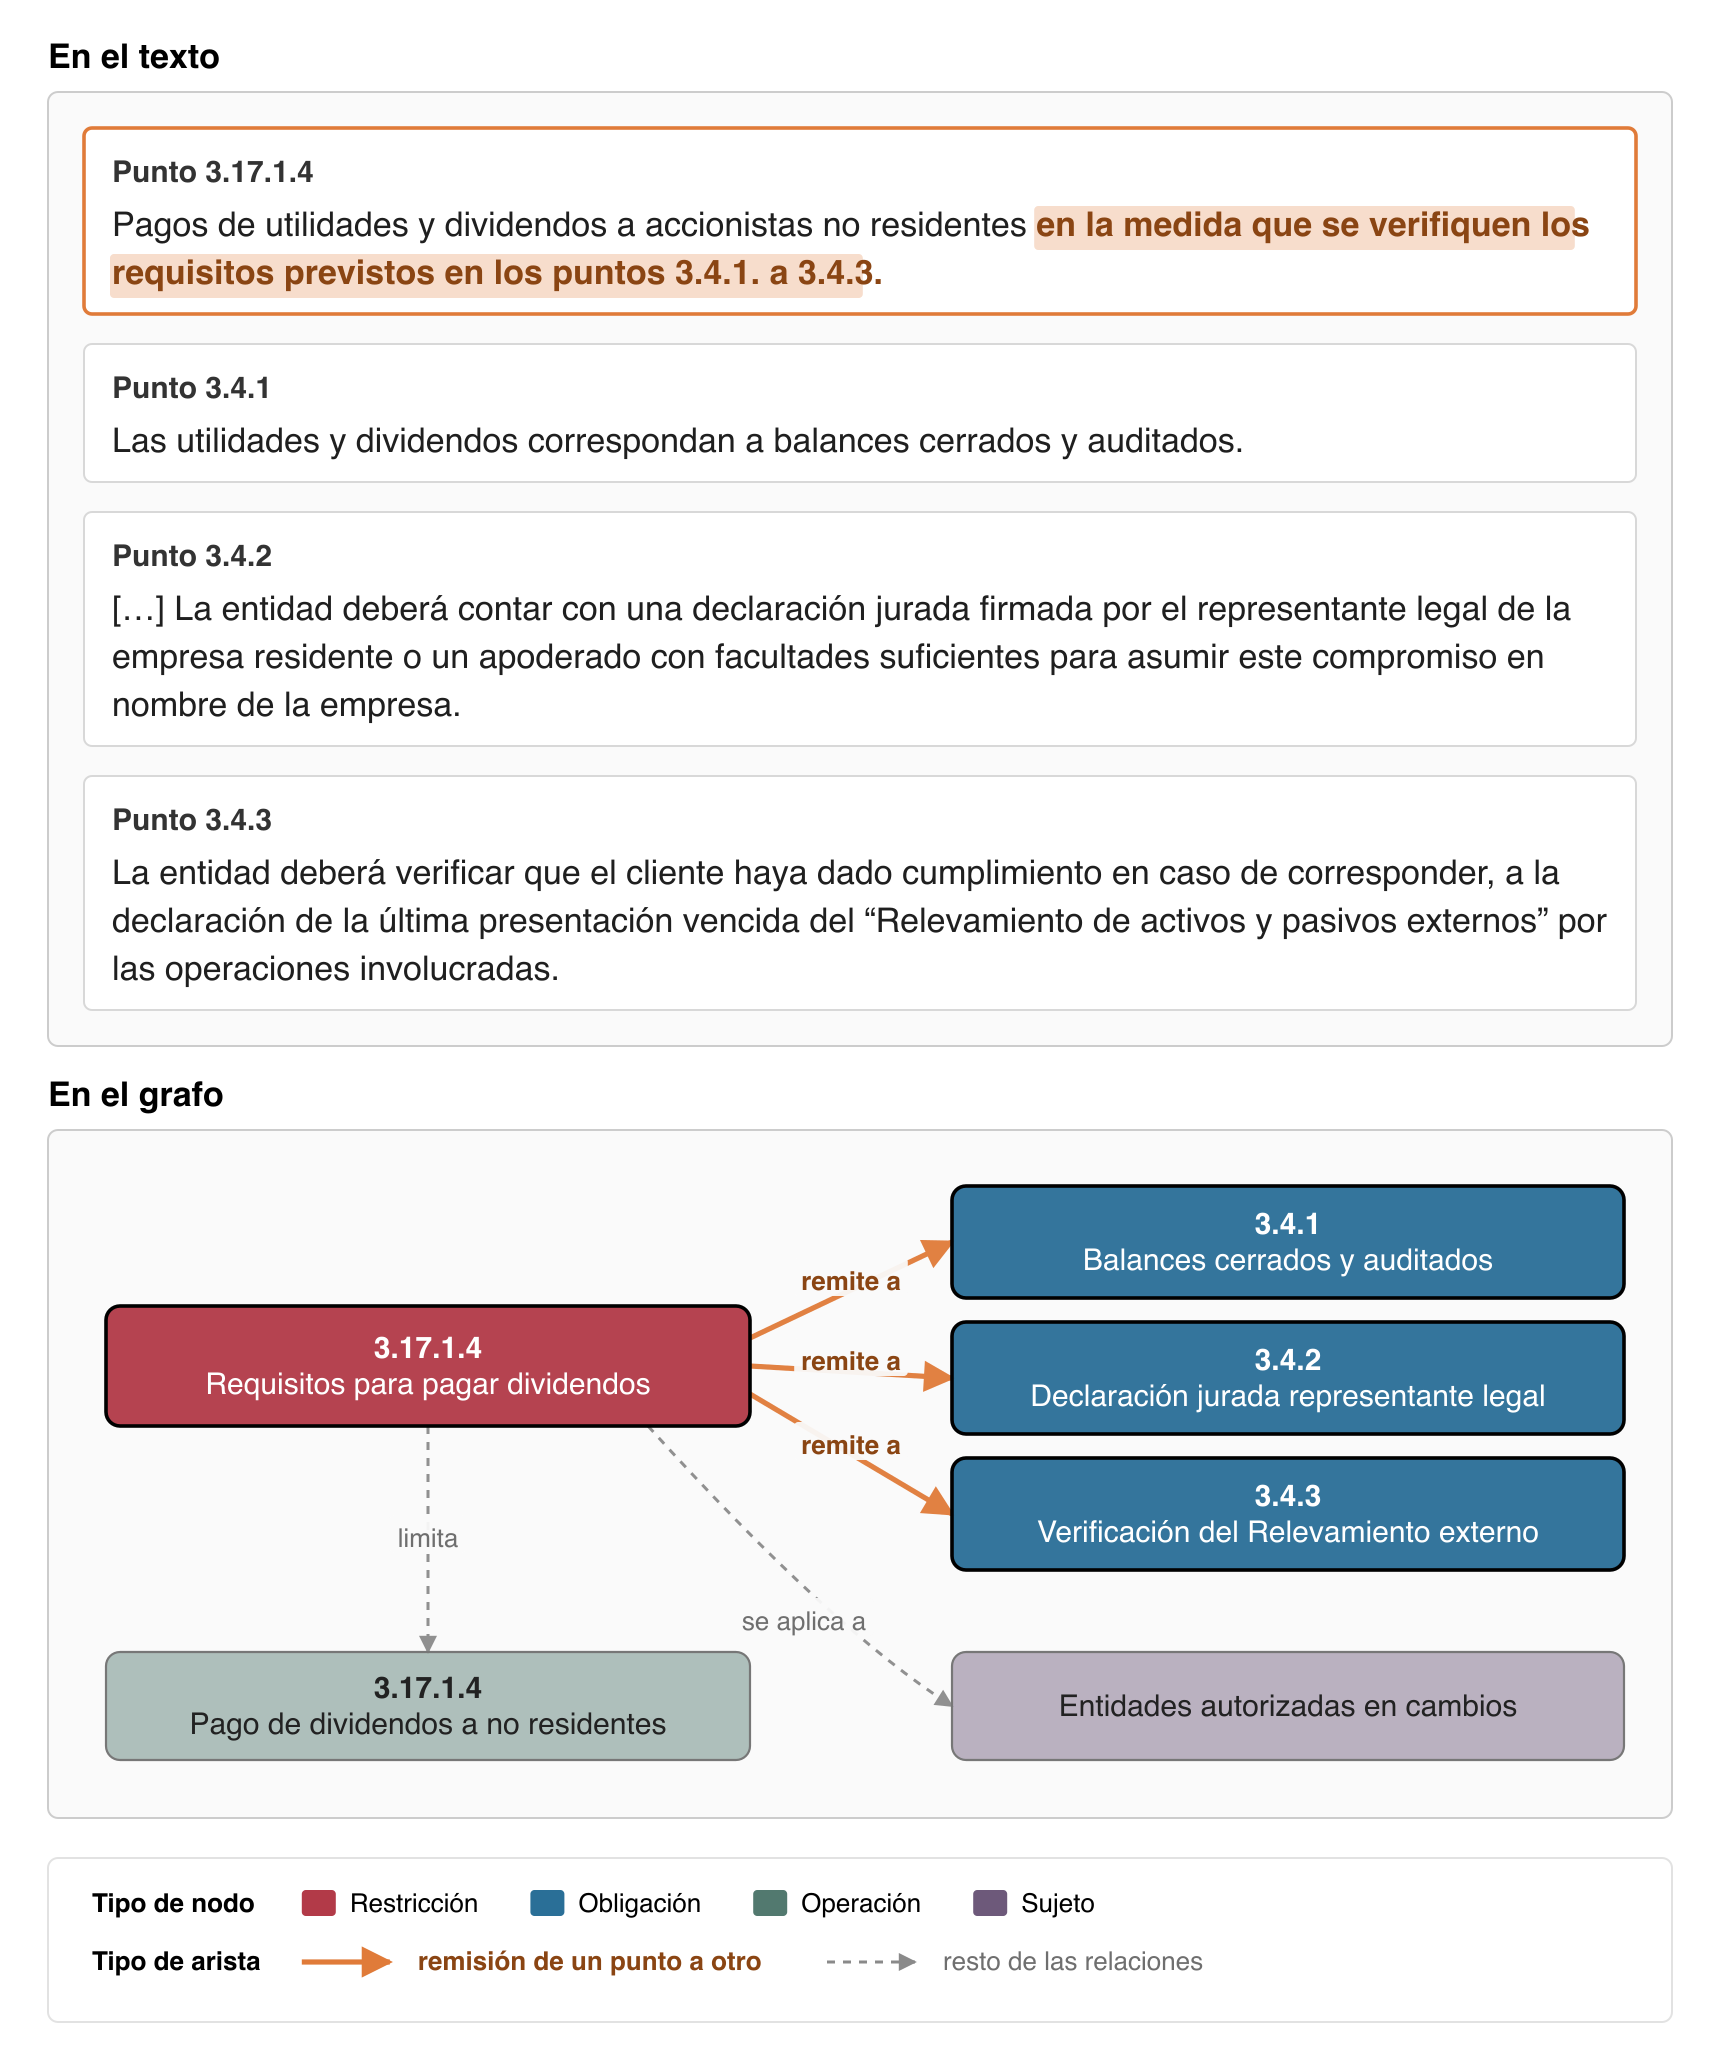
\includegraphics[width=0.85\linewidth]{figuras/figura_norma_a_grafo.png}
  \caption[De la norma al grafo]{Un punto de la normativa y su
    representación en el grafo. Arriba, el texto del punto 3.17.1.4 del
    Texto Ordenado de Exterior y cambios, con la frase que remite a otros
    tres puntos resaltada, y el texto de esos tres puntos. Abajo, el mismo
    contenido como grafo, donde el color de cada nodo indica su tipo, cada
    arista lleva el nombre de la relación, cada nodo indica de qué punto
    proviene y las tres aristas resaltadas son la remisión.}
  \label{fig:norma_a_grafo}
\end{figure}

Los sistemas que hoy responden preguntas sobre colecciones de documentos siguen, en su mayoría, un enfoque llamado generación aumentada por recuperación (retrieval-augmented generation, RAG) \cite{lewis2020rag}. El sistema corta los documentos en fragmentos, busca los más parecidos a la pregunta y pide a un modelo de lenguaje que redacte una respuesta a partir de ellos. Sobre un conjunto de documentos como el del BCRA, un corpus, ese enfoque tiene dos limitaciones. La primera es que la búsqueda no sigue las remisiones. En el ejemplo anterior, el fragmento que contiene el punto que autoriza el pago de dividendos trae la frase que remite a los otros tres puntos, pero no el texto de esos puntos, que está en otro fragmento. Ese otro fragmento se recupera solo si se parece a la pregunta, y un punto que obliga a verificar una declaración del cliente no se parece a una pregunta sobre pago de dividendos. El sistema redacta entonces la respuesta sin las condiciones que la norma exige. La segunda limitación es que recuperar el fragmento correcto no garantiza responder bien. La forma habitual de evaluar estos sistemas mira solo el primer paso, es decir, si entre lo recuperado estaba el fragmento correcto, y el segundo paso también puede fallar. El modelo puede tener el fragmento correcto y aun así redactar una respuesta equivocada, por ejemplo, omitiendo una condición que el fragmento original sí incluía. Una evaluación que solo mira lo recuperado da esa respuesta por buena.

La dificultad es entonces doble: seguir la norma a través de sus remisiones y sus salvedades, y saber si la respuesta obtenida es correcta.

Lo primero pide una forma de guardar la normativa en la que el texto no se parta en fragmentos de tamaño arbitrario sino en los puntos que el propio Texto Ordenado define, en la que cada regla lleve consigo a quién se aplica y de qué punto proviene, en la que una excepción quede unida por una relación explícita a la regla que exceptúa, y en la que se pueda ir de una regla a las que la completan sin depender de que se parezcan entre sí. Una representación con esas propiedades es el grafo de conocimiento (knowledge graph, KG).

Un grafo de conocimiento representa la información como nodos y aristas en lugar de documentos. Los nodos son elementos concretos, una obligación, una operación, una entidad financiera, y las aristas son relaciones con nombre y dirección entre dos nodos, como que una restricción limita una operación o que un punto remite a otro. La Figura~\ref{fig:norma_a_grafo} muestra los dos lados del ejemplo de los dividendos. Arriba está el texto tal como aparece en el Texto Ordenado, con la frase que remite resaltada, y abajo el mismo contenido como grafo, donde los nodos son las cosas que la normativa establece, la operación, la restricción que la condiciona, las tres obligaciones y el sujeto al que se aplican, cada uno con el punto del que proviene, y las tres aristas resaltadas son la remisión. Un sistema que consulta el grafo recorre esas aristas y llega al contenido remitido, mientras que un sistema que recibe un fragmento de texto recibe la frase y no lo que esta señala. La Figura~\ref{fig:fragmentos_vs_grafo} muestra qué tiene a la vista cada sistema al responder la pregunta del ejemplo.

\begin{figure}[H]
  \centering
  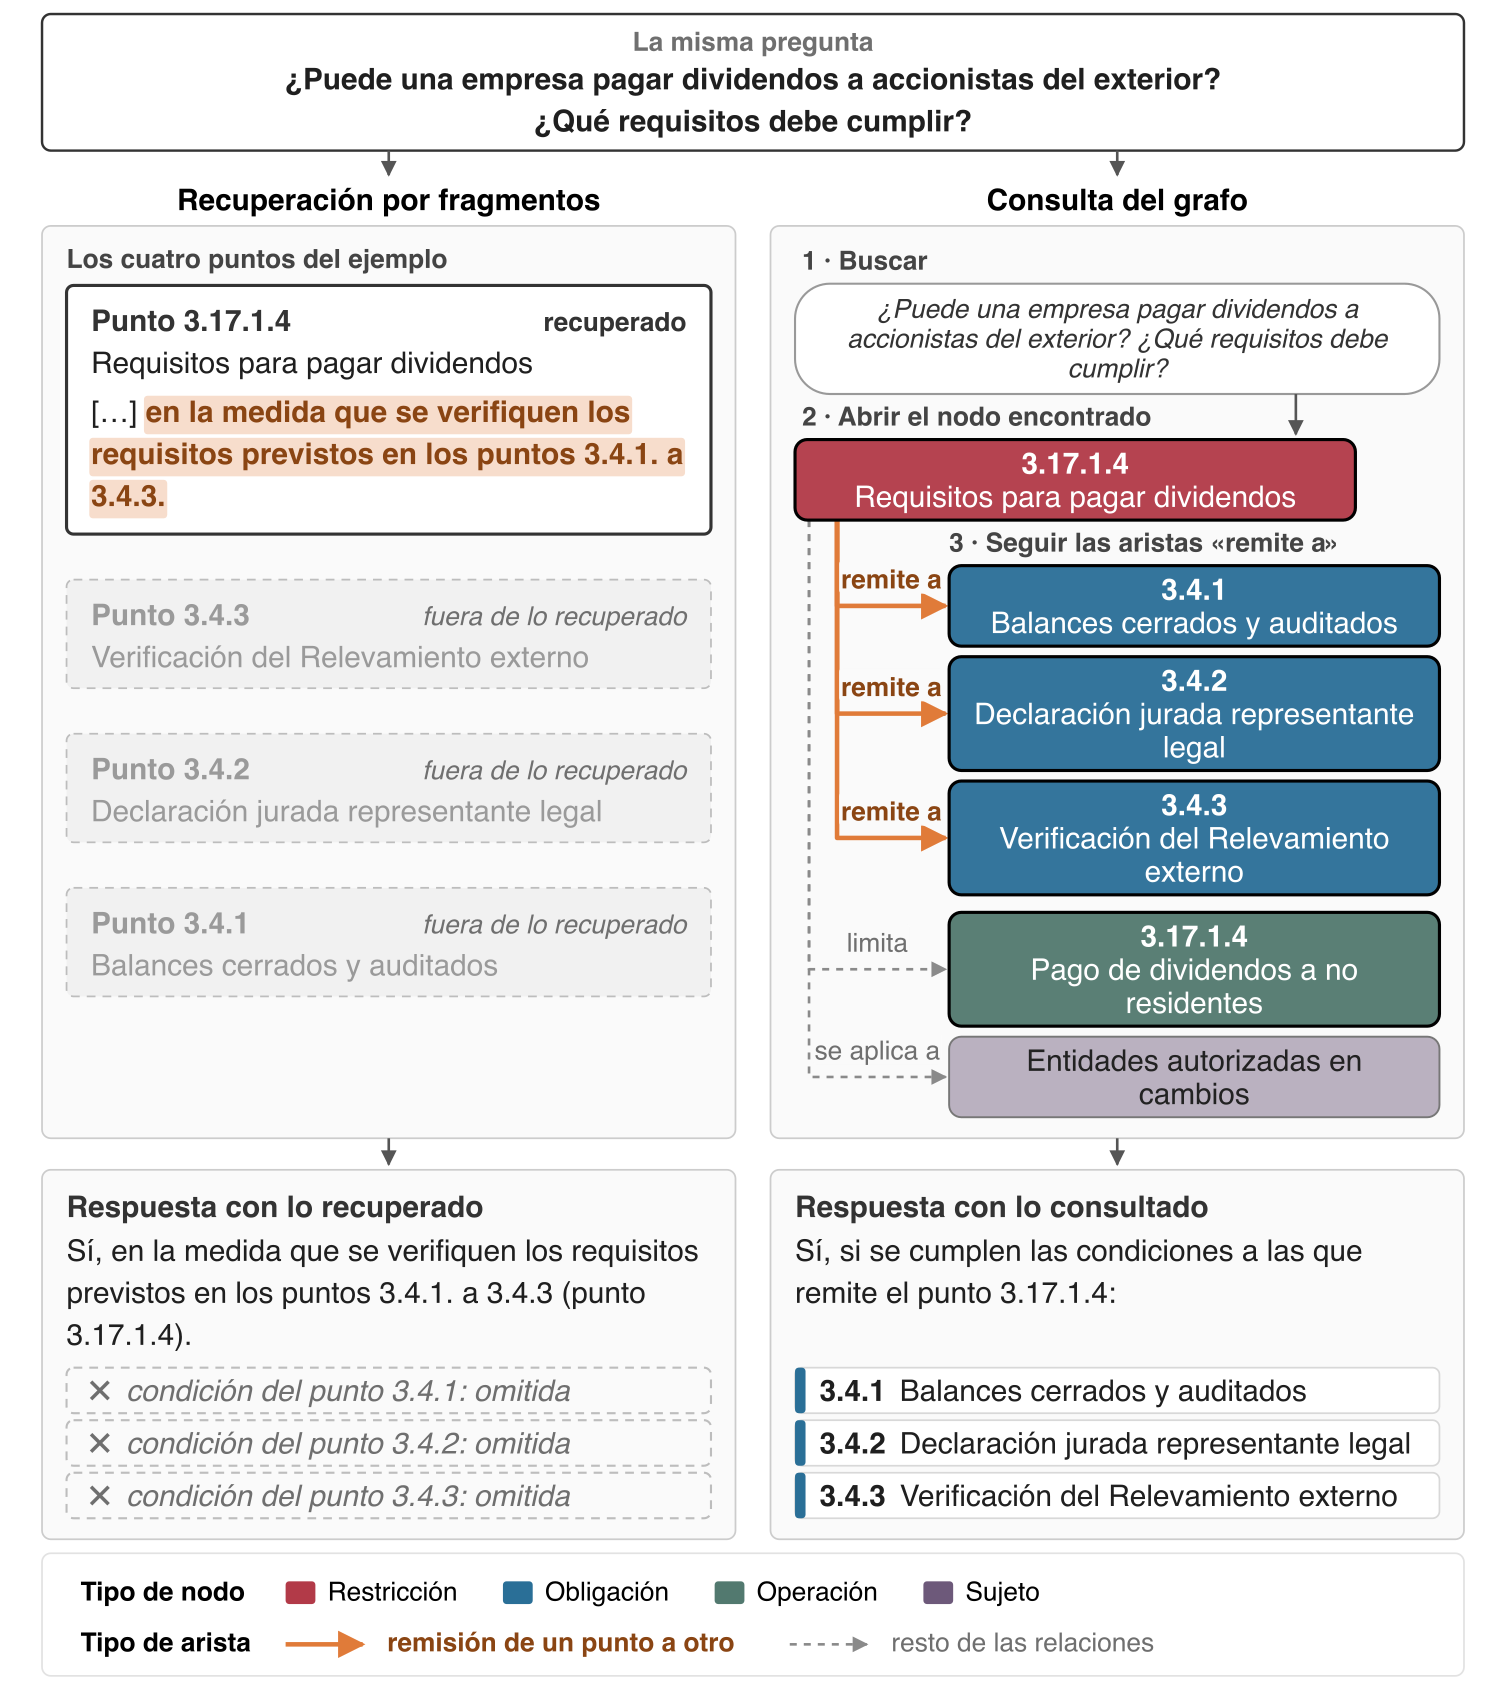
\includegraphics[width=\linewidth]{figuras/figura_fragmentos_vs_grafo.png}
  \caption[Fragmentos contra grafo]{La misma pregunta con dos formas de
    consultar la normativa. A la izquierda, los cuatro puntos de la Figura~\ref{fig:norma_a_grafo} según los devolvería o no una búsqueda por texto sobre la pregunta, y la
    respuesta que puede redactarse solo con lo recuperado; a la derecha,
    el recorrido por el grafo desde el punto que autoriza hasta las tres
    obligaciones a las que remite. Esquema del mecanismo; la comparación
    medida está en el Capítulo~\ref{cap:comparacion}.}
  \label{fig:fragmentos_vs_grafo}
\end{figure}

Construir un grafo sobre un corpus especializado exigía hasta hace poco un trabajo manual considerable, y aquellos construidos a mano envejecían a medida que cambiaba lo representado \cite{suchanek2007yago}. Sin embargo, los modelos de lenguaje de gran escala (large language models, LLM) cambiaron esa situación. Un modelo puede leer un texto y extraer de él entidades y relaciones, sea con un conjunto de tipos definido de antemano o dejando que el propio modelo los proponga \cite{carta2023iterative}, y varios modelos pueden encadenarse para extraer y verificar sobre colecciones grandes de documentos \cite{lu2025karma}. La automatización no elimina los errores de extracción, y por eso saber cuánto se puede confiar en el grafo resultante pasa a ser parte del problema.

Un recurso que sirviera para responder sobre esta normativa tendría entonces que ser un KG construido sobre el corpus completo, con sus obligaciones, restricciones, excepciones y operaciones y los sujetos a los que se aplican, con el punto del texto oficial del que proviene cada elemento, y tendría que publicarse acompañado de la evidencia de cuánto se puede confiar en él, tanto en su contenido como en las respuestas que se apoyan en él, juzgadas por lo que responden y no solo por lo que recuperan. Hasta donde se ha relevado, no existe un recurso público con esas propiedades para la regulación del BCRA.

\section{Un grafo de conocimiento para la regulación del BCRA}
\label{sec:propuesta}

Este trabajo construye ese recurso y el método para evaluarlo. El recurso es un grafo de conocimiento de la normativa del BCRA en el que cada elemento registra su procedencia en el texto oficial. Para responder preguntas se usa un agente, es decir, un modelo de lenguaje que consulta el grafo paso a paso con tres operaciones: buscar nodos por palabras, abrir un nodo y listar sus vecinos. La evaluación cubre tanto el contenido del grafo como las respuestas que se apoyan en él y, cuando una respuesta falla, determina si la falla se originó en el grafo o en el agente.

El grafo se construye con un proceso por etapas. Cada Texto Ordenado se divide siguiendo su propia estructura de secciones y puntos. Un modelo de lenguaje extrae de cada parte las entidades y relaciones que admite un esquema fijo de nueve tipos de entidad y trece tipos de relación. Un segundo
modelo revisa cada extracción contra el texto del que salió, devuelve a extraer lo que quedó incompleto y marca lo que aun así requiere revisión humana. Las partes se unen después en un único grafo mediante un procedimiento determinístico, de modo que, a partir de las mismas extracciones, el ensamblado produce siempre el mismo grafo. Sobre ese grafo ya ensamblado se resuelven las remisiones. Cada referencia que un punto hace a otro se convierte en una arista cuando el punto citado puede localizarse en el corpus, y queda registrada como no resuelta cuando no. La Figura~\ref{fig:proceso_extraccion} resume ese proceso.

\begin{figure}[H]
  \centering
  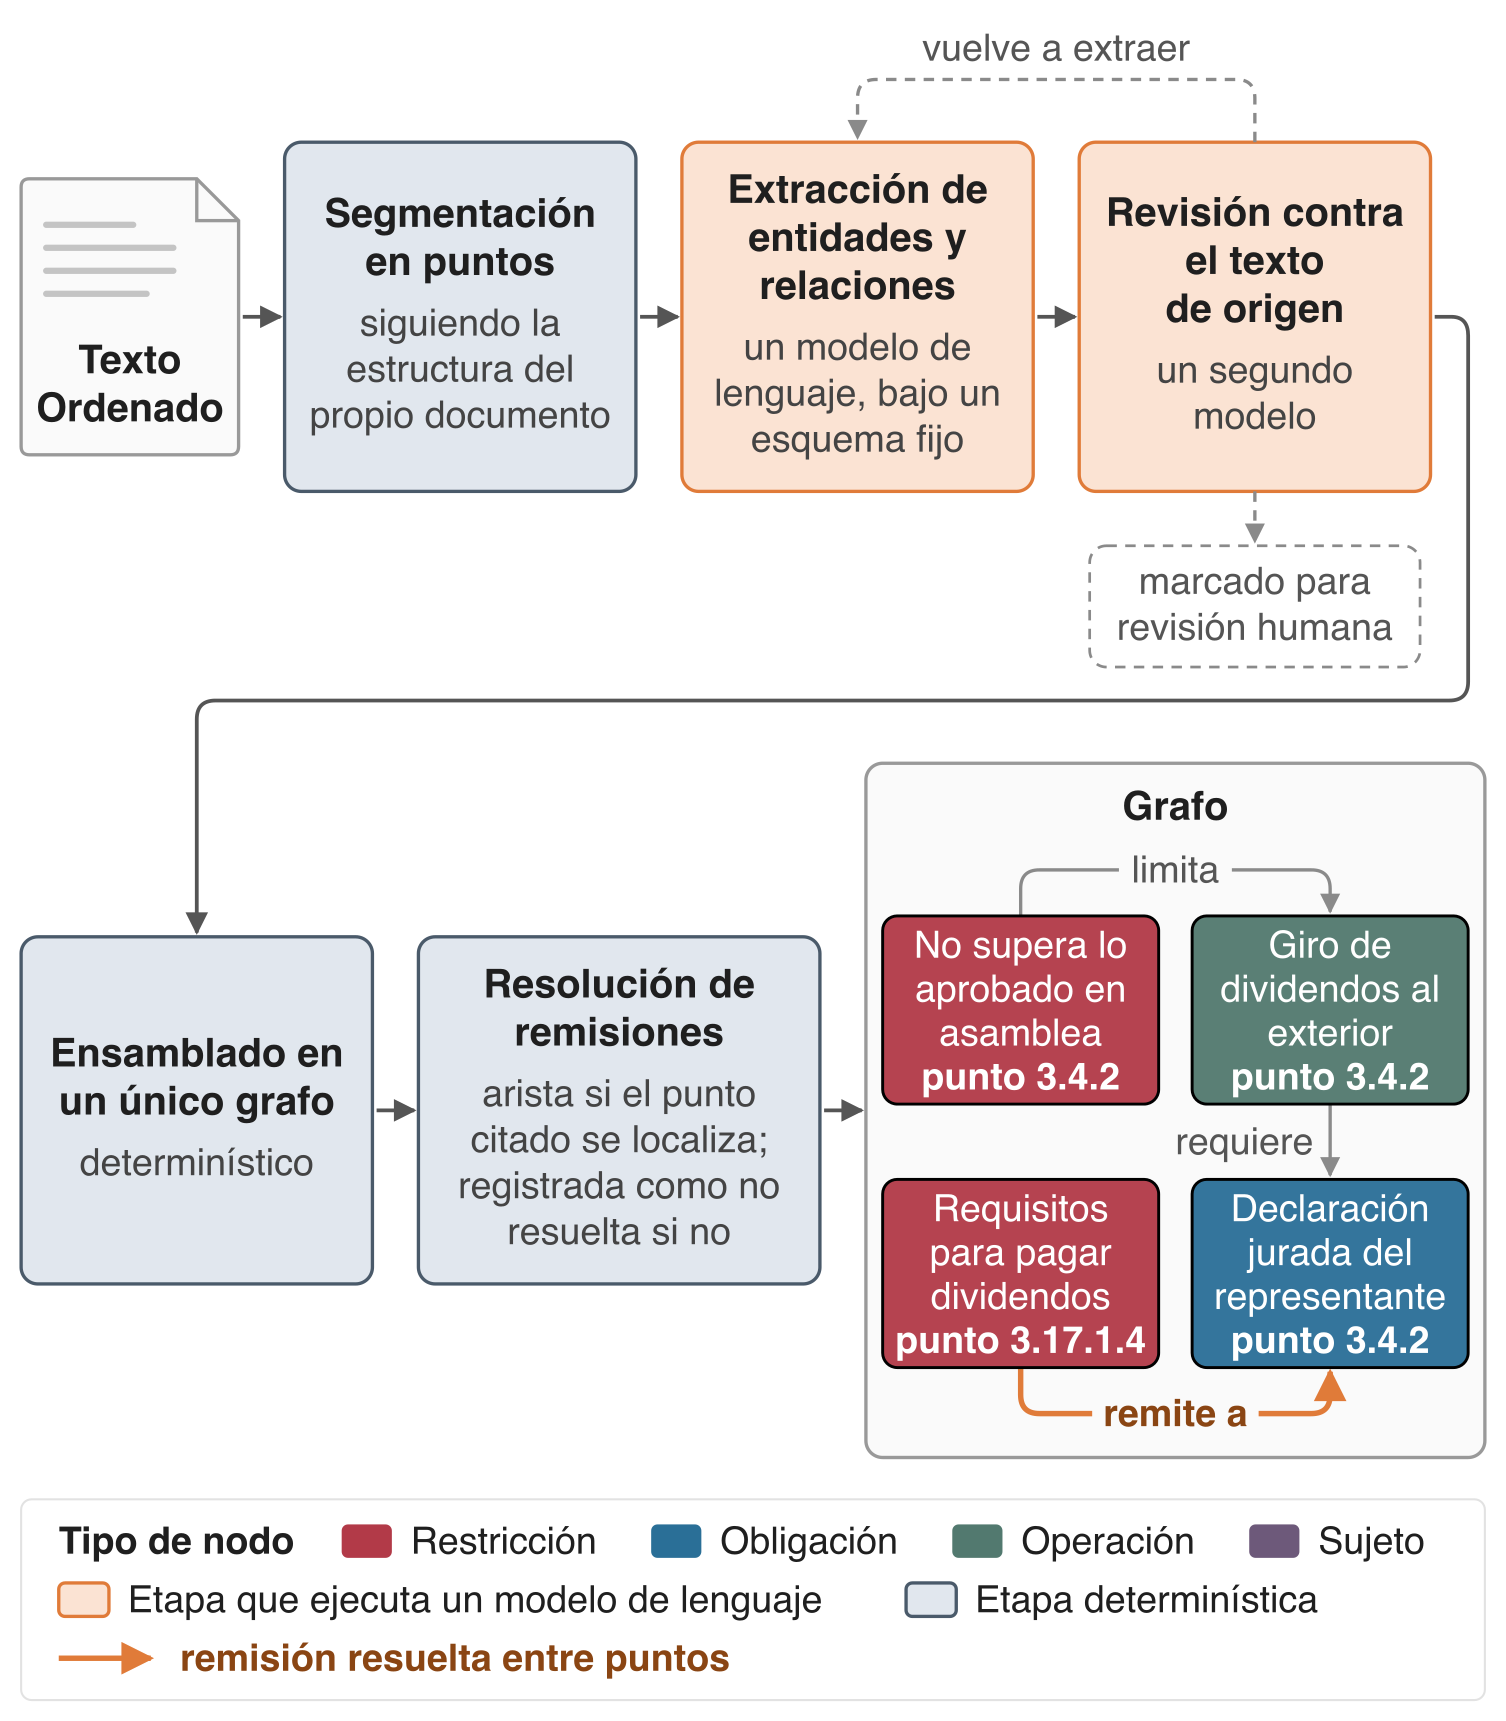
\includegraphics[width=0.85\linewidth]{figuras/figura_proceso_extraccion.png}
  \caption[Del documento al grafo]{Del documento al grafo. Cada Texto
    Ordenado se segmenta según su estructura, un modelo extrae entidades y
    relaciones bajo el esquema fijo, un segundo modelo revisa cada
    extracción contra su texto, y un procedimiento determinístico ensambla
    el grafo y resuelve las remisiones. Cada nodo conserva el punto del
    que proviene.}
  \label{fig:proceso_extraccion}
\end{figure}

\textcolor{red}{Aca falta un parrafo con el resultado final sobre todo el corpus y por ahi una tablita con los numeros del grafo}

% [PENDIENTE: un párrafo con el resultado
% sobre el corpus completo y la Tabla~\ref{tab:grafo_escalado}. Ningún
% número entra hasta que exista el grafo escalado; los del conjunto de
% desarrollo (6.529 nodos / 17.772 aristas sobre 5 documentos) van al
% capítulo de construcción, no acá.]
% \begin{table}[H]
%   \centering\small
%   \caption[El recurso]{El recurso. Documentos y páginas cubiertos,
%     unidades extraídas, nodos por tipo, aristas por relación, remisiones
%     resueltas y no resueltas, y costo de construcción.}
%   \label{tab:grafo_escalado}
%   \begin{tabular}{lr}\toprule
%   Documentos cubiertos & \\ Páginas & \\ Unidades extraídas & \\
%   Nodos (por tipo) & \\ Aristas (por relación) & \\
%   Remisiones resueltas / no resueltas & \\ Costo de construcción (USD) & \\
%   \bottomrule\end{tabular}
% \end{table}

% Se completa con la primera tanda del escalado (B6.1) y se cierra con B6.4.

Evaluar un grafo construido automáticamente es difícil porque no existe una versión correcta contra la cual compararlo, y evaluar las respuestas que se apoyan en él es difícil porque una respuesta puede estar anclada en la fuente correcta y aun así ser incorrecta. Este trabajo sella el diseño de cada evaluación antes de mirar resultado alguno y valida sus instrumentos contra lectura humana. Sobre el contenido del grafo, una muestra de sus hechos se juzga contra el pasaje del texto oficial del que cada hecho dice provenir, por su corrección y por su importancia, y su cobertura se estima buscando en el grafo los hechos que cada pasaje establece, siguiendo el precedente de los grafos de gran escala construidos automáticamente \cite{suchanek2007yago}. Sobre el uso, un conjunto de preguntas, cada una con el punto del texto oficial que la responde y sus criterios de corrección, fijado de antemano, mide la fidelidad de las respuestas del agente; un modelo de lenguaje actúa como juez y su acuerdo con una lectura humana independiente se mide antes de usarlo, y un procedimiento determinístico comprueba, para cada respuesta, que los puntos que cita existen, fueron consultados y coinciden con el punto que la responde. Para cada respuesta fallida, un procedimiento determinístico sobre el registro de lo que el agente consultó establece si el contenido faltaba en el grafo, si el agente no llegó a él, si lo vio sin abrirlo o si lo consultó y aun así respondió mal. Esa distinción es la que ningún trabajo relevado hace, y es la que permite saber si una falla se corrige mejorando el grafo o mejorando el agente.

La comparación contra un sistema de recuperación por fragmentos se hace con el mismo agente sobre el mismo corpus, cambiando únicamente aquello que el agente puede consultar. Todo lo que se mide sobre el conjunto de desarrollo es el material con el que se afinó el método y el instrumento. La medición que cuenta se hace una sola vez, sobre el grafo escalado, con preguntas nuevas construidas sobre documentos que no intervinieron ni en el desarrollo ni en la validación del esquema, con la comparación contra fragmentos como brazo declarado, y con su diseño sellado antes de correr.

\textcolor{red}{Falta un overview de resultados etc}
% [TODO] la evaluación intrínseca por tripletas y el head-to-head están
% decididos (reunión 26/08) pero todavía no corridos. 
% [PENDIENTE B6.3: overview de resultados. Entra
% cuando exista la medición sobre el grafo escalado (fidelidad, atribución,
% tripletas y comparación contra fragmentos). Regla: dos o tres cifras de
% titular, sin volcado; lo de desarrollo (11 de 12; 46–69 %) ya está en las
% contribuciones 3 y 4 con su fila del mapa. Lo que corrió y lo que no, por
% componente, en el inventario de U-INV-EVAL.]

\section{Objetivos y alcance del trabajo}

\subsection{Objetivo general}

Construir un grafo de conocimiento de la normativa del Banco Central de la República Argentina en el que cada elemento registre su procedencia en el texto oficial, y establecer con qué confianza puede usarse, evaluando tanto su contenido como las respuestas que se apoyan en él, y demostrar su utilidad en la reconstrucción de la cadena de normas que justifica una restricción operativa.

\subsection{Objetivos específicos}

\begin{enumerate}
  \item Diseñar un esquema que capture las entidades y relaciones propias de la normativa del BCRA, y validarlo sobre documentos ajenos al conjunto de desarrollo antes de aplicarlo al corpus completo.

  \item Construir el grafo sobre el corpus completo de Textos Ordenados mediante un proceso por etapas, con el punto del texto oficial del que proviene cada nodo y cada arista.

  \item Diseñar un método de evaluación, sellado antes de correr, que mida la calidad del contenido del grafo contra el texto del que proviene, la fidelidad de las respuestas de un agente que lo consulta y la exactitud de sus citas, y el origen de cada falla, en el grafo o en el agente.

  \item Medir con ese método el recurso construido sobre el corpus completo, y compararlo contra un sistema de recuperación por fragmentos sobre el mismo corpus.

  \item Implementar y evaluar un sistema que, dado un registro de operaciones de una entidad o un cliente, reconstruya sobre el grafo la cadena de normas que justifica una restricción operativa.
  
  \item Implementar y probar la actualización del recurso ante cambios en la normativa: un proceso periódico que detecte qué documentos cambiaron en la fuente, determine qué elementos del grafo dependen de ellos y los vuelva a extraer, probado contra la diferencia entre el corpus descargado al inicio del trabajo y la fuente vigente.
\end{enumerate}
% Objetivo 6: actualización por REEMPLAZO
% DE DOCUMENTO. Cuando el monitor señala un Texto Ordenado cambiado, se
% re-corre el proceso completo solo sobre ese documento, se retira del
% grafo todo elemento cuya procedencia lleve ese archivo, se inserta lo
% nuevo, se vuelven a resolver las remisiones (las que salen del documento
% y las que desde otros apuntan a sus puntos), y el resultado pasa por el
% mismo gate que cualquier release (shapes + regression). Prueba: los
% documentos que el monitor ya reporta cambiados desde la descarga
% original, contra el recurso completo; se reporta qué entró, qué salió y
% qué remisiones cambiaron de destino.
% MEJORA POSTERIOR, no comprometida (para el cierre del proyecto o trabajo
% futuro): actualización por DIFERENCIA DE PUNTOS. Comparar la estructura
% vieja y nueva del documento punto por punto, re-extraer solo las unidades
% cuyo texto o cuya cadena de encabezados cambió, y conservar el resto.
% Lo que hay que resolver antes de hacerla: (1) un punto contenedor que
% cambia arrastra a sus hijos por la herencia de encabezados; (2) el
% ensamblado fusiona entre unidades, así que un nodo puede tener
% procedencia en un punto cambiado y en uno intacto; (3) la renumeración
% de puntos rompe la identidad por (archivo, punto) y exige un pareo
% viejo→nuevo antes de decidir qué se conserva. Ahorra API respecto del
% reemplazo; no cambia el gate.

El alcance del trabajo queda fijado por tres decisiones. El corpus es el conjunto de Textos Ordenados vigentes al momento del relevamiento, con cada documento identificado por su huella criptográfica, y un proceso periódico compara la fuente contra esas huellas y señala qué documentos cambiaron, de modo que el recurso representa una versión fechada de la normativa y queda registrado desde cuándo dejó de estar al día. El grafo representa lo que la norma establece, con el punto del que proviene cada elemento, y no una interpretación jurídica de ella. Y la vigencia en el tiempo, la norma que modifica o deroga a otra, queda fuera del alcance de esta versión del recurso, que se mantiene al día por reemplazo de los documentos que cambian y no por historia de sus versiones.

\section{Aportes y organización del informe}
\label{sec:contribuciones}

El capítulo~\ref{cap:marco} revisa los trabajos previos y deja a la vista cuatro vacíos. Ningún trabajo relevado mide con un instrumento validado contra juicio humano la fidelidad de las respuestas que un grafo permite dar ni la exactitud con que citan su fuente, ni distingue una falla del grafo de una falla de quien lo consulta. Las comparaciones publicadas entre grafos y recuperación por fragmentos carecen de un término de referencia independiente. Los corpus evaluados en la etapa de los modelos de lenguaje están en inglés, sin evidencia sobre normativa en castellano. Y los costos de construcción y de consulta rara vez se reportan. Sobre esos vacíos se apoyan las contribuciones que siguen.

Las contribuciones de este trabajo son cinco.

\begin{enumerate}
  \item \textbf{Un esquema de modelado para la normativa del BCRA, validado
    antes de escalar}, con nueve tipos de entidad, trece tipos de relación
    y un catálogo cerrado de sujetos que resuelve a quién se dirige cada
    norma, puesto a prueba por lectura sobre documentos ajenos al conjunto
    de desarrollo y congelado con sus límites declarados.
    Capítulo~\ref{cap:esquema}.
% Fuente: 9/13 verificados contra prompt_congelado.py (mapa fila 109 y
% laudo 2593d4d); catálogo y roles de alcance, filas 41–53 y 123–129.

  \item \textbf{Un grafo de conocimiento de la normativa del BCRA en el que
    cada nodo y cada arista registran su procedencia}, construido con un
    proceso por etapas bajo ese esquema y publicado junto con la evidencia
    de cuánto se puede confiar en él. Capítulo~\ref{cap:construccion}.
% Los tamaños del conjunto de desarrollo (6.529/17.772) van al capítulo de
% construcción, no acá.
% [TODO: escala final del recurso cuando exista el grafo escalado]

  \item \textbf{Un conjunto de evaluación para preguntas sobre normativa
    del BCRA}, compuesto por 40 preguntas, cada una con el punto del texto oficial que la responde y sus criterios de corrección, 164 en total, fijado antes de correr
    cualquier experimento y utilizable con independencia del grafo.
    Capítulo~\ref{cap:fidelidad}.
% Fuente: mapa fila 16.

  \item \textbf{Un método para evaluar un grafo de conocimiento
    construido automáticamente y las respuestas que se apoyan en él},
    que combina el juicio de una muestra de los hechos del grafo contra
    el texto del que provienen, un juez automático validado contra una
    lectura humana independiente (acuerdo en 11 de 12 respuestas) y un
    procedimiento determinístico que atribuye cada falla a la ausencia
    del contenido en el grafo, a que el agente no llegó a él, a que lo
    vio sin abrirlo o a que lo consultó y aun así respondió mal.
    Capítulos~\ref{cap:fidelidad} y~\ref{cap:atribucion}.
% Fuente: mapa fila 2. El muestreo de hechos va sin número hasta que la
% corrida exista.

  \item \textbf{El hallazgo de que tener a la vista el contenido correcto
    no garantiza responder bien.} Sobre el conjunto de desarrollo, entre
    el 46\,\% y el 69\,\% de las respuestas fallidas, según la versión
    del grafo, ocurrieron con el contenido correcto ya consultado por el
    agente. Capítulo~\ref{cap:atribucion}.
% Fuente: mapa fila 17 (17/37, 25/36, 21/36).
\end{enumerate}
% [TODO: contribuciones pendientes de resultados — no se listan hasta que
% existan: evaluación sobre el corpus escalado (B6.3), resultado de la
% comparación contra recuperación por fragmentos, resultado de la
% evaluación por tripletas, el sistema de explicabilidad (objetivo 5) y la
% actualización del recurso ante cambios (objetivo 6), si corren. Los
% métodos de las dos primeras ya se anuncian en §1.2; lo que falta es el
% resultado.]

% [PENDIENTE: organización del informe. Un párrafo por capítulo, en el
% orden del índice, cuando la estructura quede fija: el estado del arte va en §2.5–2.6 (decisión 17/09) y del laudo
% sobre el capítulo de explicabilidad. Al escribirlo, reemplazar el bloque
% de estructura tentativa que sigue, que ya está viejo: el capítulo 3 es
% el esquema y su validación, el 4 la construcción, y falta el de
% explicabilidad.]

\chapter{Marco teórico y estado del arte}
\label{cap:marco}

Este capítulo explica los grafos de conocimiento, su construcción, su evaluación y otros enfoques alternativos. Primero define qué es un grafo de conocimiento, cómo se construye a partir de texto y cómo se evalúa, y fija la definición que el capítulo~\ref{cap:esquema} instancia. La sección~\ref{sec:mt_rag} presenta la generación aumentada por recuperación, que es el enfoque contra el que este trabajo se compara. La sección~\ref{sec:mt_agente} explica qué es un agente que consulta un grafo con herramientas, y la sección~\ref{sec:mt_eval} cómo se evalúan sus respuestas con un modelo de lenguaje como juez y cómo se atribuye una falla. La sección~\ref{sec:estado_arte} revisa los trabajos previos en tres frentes, la extracción de información sobre textos regulatorios y legales, las comparaciones entre recuperación por fragmentos y grafos en ese dominio, y los grafos publicados como recurso, y la sección~\ref{sec:vacios} enuncia los vacíos que esa revisión deja y en los que este trabajo se ubica.

\section{Grafos de conocimiento}
\label{sec:mt_kg}

\subsection{Qué es un grafo de conocimiento}

Un grafo de conocimiento (knowledge graph, KG) es un grafo de datos cuyos nodos representan entidades y cuyas aristas representan relaciones entre ellas \cite{hogan2021kg}. Una entidad es cualquier cosa de la que el texto habla y a la que se puede volver a referir, como una obligación, una operación, una entidad financiera o un Texto Ordenado en la normativa del BCRA. Una relación es un vínculo entre dos entidades que tiene nombre y dirección, de modo que \texttt{limita} va de una restricción a una operación y no al revés. La unidad mínima de información es la tripleta formada por un nodo de origen, la arista o relación y un nodo de destino, y se lee como una afirmación. En el ejemplo de la introducción, la tripleta (restricción del punto 3.17.1.4, \texttt{limita}, pago de dividendos a no residentes) afirma que esa restricción limita esa operación, y la tripleta (restricción del punto 3.17.1.4, \texttt{referencia}, obligación del punto 3.4.2) afirma que remite a esa obligación. La Figura~\ref{fig:norma_a_grafo} muestra cinco de esas tripletas alrededor de un mismo nodo, y la Figura~\ref{fig:tripleta} descompone la primera.

\begin{figure}[H]
  \centering
  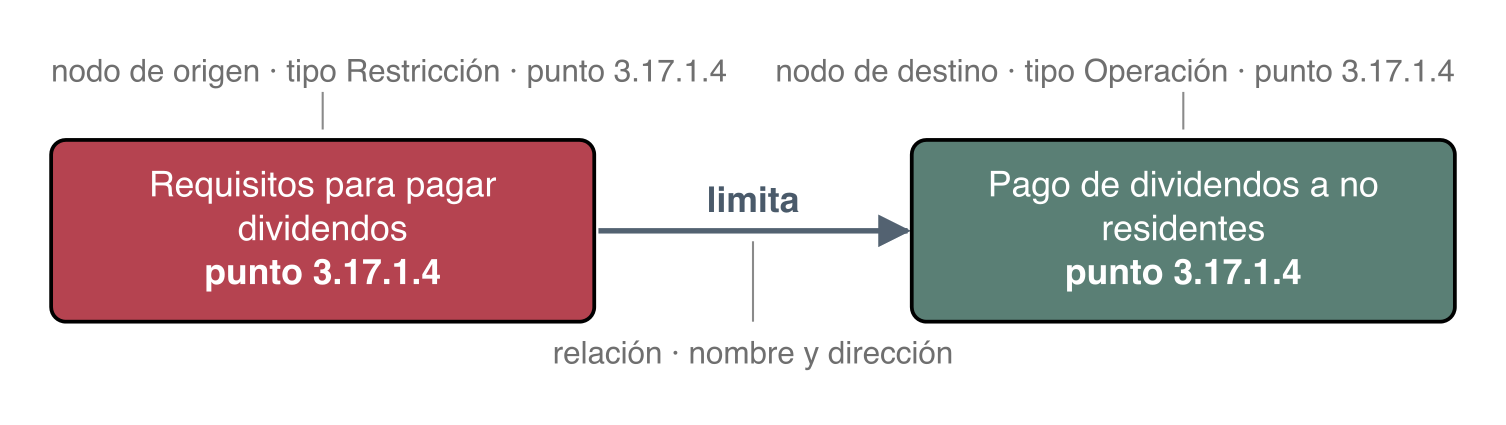
\includegraphics[width=0.6\linewidth]{figuras/figura_tripleta.png}
  \caption[Una tripleta]{Una tripleta ejemplo del KG construido en este trabajo. El nodo de origen (rojo) y el de
    destino (verde) son entidades con tipo y con el punto del que provienen; la arista es una relación con nombre y dirección. Como afirmación se lee de la siguiente manera: "La restricción del punto 3.17.1.4 limita el pago de dividendos a no residentes, operación del mismo punto".}
  \label{fig:tripleta}
\end{figure}

Dos rasgos distinguen a un grafo de conocimiento de otras formas de guardar la misma información. Las entidades tienen tipo, de modo que una restricción, una operación y un sujeto son cosas de distinta clase aunque las tres sean nodos. Un índice de texto guarda pasajes y responde por parecido; una base de datos relacional guarda filas en tablas fijas y responde por coincidencia de valores; un grafo guarda afirmaciones y responde recorriéndolas, de una entidad a las que están unidas a ella. El vocabulario de tipos de entidad y de nombres de relación que un grafo admite es su esquema, y el capítulo~\ref{cap:esquema} presenta el de este trabajo.

\subsection{Construcción del KG}

Construir un grafo a partir de documentos es un problema de extracción de información, y sigue siempre los mismos pasos, cualquiera sea la técnica con que se ejecute cada uno. El documento se divide en unidades de texto manejables. En cada unidad se identifican las menciones de entidades y se les asigna un tipo, de modo que \enquote{la entidad deberá contar con una declaración jurada} produce un nodo de tipo obligación. Entre las entidades de la unidad se identifican las relaciones, cada una con nombre y dirección, de modo que la misma unidad produce una arista de esa obligación hacia el sujeto al que obliga. Las menciones que nombran la misma entidad con formas distintas se resuelven en un único nodo, las unidades se ensamblan en un solo grafo, y cada nodo y cada arista conservan el registro de la unidad de la que salieron. La Figura~\ref{fig:proceso_extraccion} de la introducción muestra esos pasos tal como este trabajo los ejecuta.

Un grafo se puede construir a partir de tres tipos de fuentes. La primera es la información ya estructurada, como las fichas y categorías de Wikipedia de las que YAGO extrajo sus primeros hechos con reglas fijas y midió su precisión sobre una muestra juzgada a mano \cite{suchanek2007yago}. La segunda es el texto libre, del que las entidades y las relaciones se extraen con sistemas que encadenan módulos especializados, sea bajo un vocabulario fijado de antemano, como hicieron Khetan et al. sobre regulación financiera \cite{khetan2021kganchored}, sea sin vocabulario previo, con cualquier expresión verbal que una dos entidades \cite{etzioni2011open,delcorro2013clausie}. La tercera, que es la de este trabajo, es el texto libre leído por un modelo de lenguaje de gran escala, que extrae entidades y relaciones en una o varias pasadas, con o sin un esquema dado, y cuya salida puede verificarse con otro modelo antes de ingresar al grafo \cite{carta2023iterative,lu2025karma}.

Con un modelo de lenguaje como extractor, la decisión de diseño central es cuánto vocabulario se le impone. En un esquema cerrado el extractor no propone vocabulario sino que elige dentro de uno fijo, cada relación declara qué tipos admite en cada extremo, y lo que el extractor produce fuera de ese vocabulario se descarta. En el extremo opuesto, el esquema abierto, el modelo propone los tipos y las relaciones que le parecen pertinentes en cada texto, y el vocabulario resultante es el que el modelo haya producido; la literatura reciente organiza los métodos según esa misma división \cite{bian2025survey}. Entre ambos cabe un esquema híbrido, que fija un núcleo de tipos y relaciones y deja que el modelo extienda el resto. Las tres variantes se comparan sobre documentos de este trabajo en la sección~\ref{sec:comparacion_esquemas}, que llama emergente a la abierta e híbrida a la intermedia. El esquema cerrado gana en consistencia y en verificabilidad, porque una tripleta con un par de tipos que el esquema no admite se rechaza sin necesidad de leerla, y pierde en cobertura, porque el contenido que no cabe en el vocabulario no produce salida y no deja rastro que contar. Hay evidencia publicada en esa dirección. En un pipeline de extracción sobre reportes operativos de desminado humanitario, guiar al modelo con una ontología de 160 tipos de entidad y 86 relaciones mejoró la exactitud de la extracción hasta un 44,2\,\%, redujo las alucinaciones hasta un 22,5\,\% y mejoró la adherencia al formato hasta un 20,9\,\%, en los tres casos frente a la peor de las configuraciones sin esa guía \cite{zhou2025textminex}.

La segunda decisión transversal es la procedencia, es decir, registrar de qué fuente sale cada hecho. YAGO la estableció como práctica al guardar, junto con cada hecho, la página y el método de los que fue extraído \cite{suchanek2007yago}, y los grafos construidos con modelos de lenguaje la conservan a nivel de artículo o de publicación (sección~\ref{sec:estado_arte}). En un texto normativo la procedencia útil es más fina, porque la cita que respalda una respuesta se da por punto, y por eso este trabajo la registra por punto del Texto Ordenado. El capítulo~\ref{cap:esquema} describe el esquema cerrado de este trabajo y cómo se midió lo que ese esquema deja afuera, y el capítulo~\ref{cap:construccion} el proceso de extracción por etapas.

\subsection{El grafo definido para este trabajo}
\label{sec:mt_kg_def}

Una tripleta no alcanza para lo que este trabajo necesita, porque no lleva consigo el tipo de sus nodos, las propiedades textuales de cada norma ni la procedencia de cada elemento. El grafo de este trabajo es por eso un grafo de propiedades dirigido y tipado, que es el modelo que implementan los motores de grafos \cite{hogan2021kg}, y se define como
\begin{equation}
  G = (V, E, \tau_V, D, \alpha, \pi).
\end{equation}
$V$ es el conjunto de nodos y $T_V$ el conjunto finito de tipos de entidad, y $\tau_V : V \to T_V$ asigna a cada nodo su tipo. $T_E$ es el conjunto finito de nombres de relación, o predicados, y $E \subseteq V \times T_E \times V$ es el conjunto de aristas, cada una una tripleta $(u, r, v)$ con nodo de origen, predicado y nodo de destino. $D \subseteq T_V \times T_E \times T_V$ es la matriz de dominio y rango, que fija qué tipo de nodo admite cada predicado en cada extremo. $\alpha$ asigna a cada nodo sus propiedades, como la descripción y el tipo de una obligación, y a cada arista las suyas, entre ellas el rol de origen, que dice si la produjo el extractor o el ensamblado. Y $\pi : V \cup E \to \mathcal{P}(L)$ es la función de procedencia, que asigna a cada nodo y a cada arista un conjunto de lugares del texto oficial, donde cada lugar de $L$ se identifica por documento, punto, unidad de extracción y páginas. El esquema es la terna $(T_V, T_E, D)$.

El esquema gobierna lo que el extractor obtiene del texto. Toda arista extraída $(u, r, v)$ cumple $(\tau_V(u), r, \tau_V(v)) \in D$, y una tripleta cuya firma no está en $D$ se rechaza antes de entrar al grafo, como muestra la sección~\ref{sec:matriz_control}. El grafo contiene además dos clases de aristas que no salen del extractor sino del ensamblado del capítulo~\ref{cap:construccion}, y que llevan en $\alpha$ un rol de origen propio. La primera son las remisiones resueltas, aristas de predicado \texttt{referencia} entre dos puntos cuando el texto de uno remite al otro, como la segunda tripleta del ejemplo de la sección anterior. La segunda son los vínculos del catálogo de sujetos, cuatro predicados que ordenan a los sujetos entre sí por subclase, instancia, pertenencia y parte, y que no figuran en $D$ porque ningún extractor los produce. El rol de origen permite separar ambas clases de las aristas extraídas en cualquier consulta.

La Tabla~\ref{tab:definicion_ejemplo} lee la tripleta de la Figura~\ref{fig:tripleta} con esos símbolos. El capítulo~\ref{cap:esquema} instancia esta definición con nueve tipos de entidad extraídos del texto más un décimo, el sujeto, tomado de un catálogo cerrado, y con trece predicados de extracción; el capítulo~\ref{cap:construccion} suma a $T_E$ los cuatro predicados del catálogo y usa $\pi$ para resolver las remisiones entre puntos, y el capítulo~\ref{cap:atribucion} la usa para saber si el agente consultó el contenido que respondía una pregunta.

\begin{table}[H]
  \centering
  \small
  \renewcommand{\arraystretch}{1.15}
\begin{tabularx}{\textwidth}{@{}l l >{\raggedright\arraybackslash}X@{}}    \toprule
    Componente & Símbolo & En la tripleta de la Figura~\ref{fig:tripleta} \\
    \midrule
    Nodo de origen & $u \in V$ & «Requisitos para pagar dividendos» \\
    Tipo del origen & $\tau_V(u)$ & \texttt{Restriccion} \\
    Predicado & $r \in T_E$ & \texttt{limita} \\
    Nodo de destino & $v \in V$ & «Pago de dividendos a no residentes» \\
    Tipo del destino & $\tau_V(v)$ & \texttt{Operacion} \\
    Firma admitida & $(\tau_V(u), r, \tau_V(v)) \in D$ & (\texttt{Restriccion}, \texttt{limita}, \texttt{Operacion}) \\
    Rol de origen & $\alpha(u, r, v)$ & extraída del texto \\
    Procedencia del origen & $\pi(u)$ & Exterior y cambios, puntos 3.17.1.4 y 3.18.1.2 \\
    Procedencia de la arista & $\pi(u, r, v)$ & Exterior y cambios, punto 3.17.1.4 \\
    \bottomrule
  \end{tabularx}
  \caption[La definición sobre un ejemplo]{Los componentes de la definición sobre la tripleta de la Figura~\ref{fig:tripleta}. La procedencia se abrevia a documento y punto; la unidad de extracción y las páginas completan cada lugar de $L$.}
  \label{tab:definicion_ejemplo}
\end{table}

\subsection{Cómo se evalúa}

Un grafo construido por extracción no tiene una versión correcta contra la cual compararse, porque producirla exigiría hacer a mano la extracción que se quiso automatizar. La evaluación se hace por eso de dos maneras que responden preguntas distintas. La evaluación intrínseca mira el contenido del grafo. Se sortea una muestra de sus hechos, cada uno se juzga contra la fuente de la que dice provenir, y la proporción de hechos correctos se reporta con un intervalo de confianza, que es el procedimiento con que YAGO evaluó sus hechos, con jueces humanos que vieron cada hecho junto a un fragmento de su página de origen y con el intervalo de Wilson al 95\,\% por relación \cite{suchanek2007yago}. Con muestras de decenas de hechos y proporciones cercanas a los extremos, ese intervalo \cite{wilson1927} cubre lo que declara y el normal cubre menos de lo que declara \cite{brown2001}. Esa vía mide la precisión de lo que está en el grafo y no lo que falta, porque la cobertura de un grafo no tiene denominador conocido y solo puede estimarse buscando en el grafo los hechos que una muestra de pasajes establece.

La evaluación extrínseca mira el uso, es decir, si un sistema responde mejor con el grafo que sin él, o que con otra forma de acceder al mismo texto. Permite comparar un grafo contra la recuperación por fragmentos, y la que reportan los trabajos que hacen esa comparación; los que publican el grafo como recurso reportan casi siempre la intrínseca (sección~\ref{sec:estado_arte}). Las dos vías no se reemplazan, porque un grafo preciso puede ser inútil si le falta lo que las preguntas necesitan, y un sistema que responde bien puede hacerlo a pesar del grafo. En un dominio especializado la evaluación intrínseca tiene además un costo propio, porque juzgar si una tripleta normativa es correcta exige leer el pasaje del que proviene, y hay tripletas que un lector sin formación en la materia no puede adjudicar. Este trabajo evalúa el grafo por las dos vías, la intrínseca con una muestra de hechos juzgados contra su pasaje y una estimación de cobertura (capítulo~\ref{cap:intrinseca}), y la extrínseca con la fidelidad de un agente sobre un conjunto de evaluación sellado (capítulo~\ref{cap:fidelidad}) y la comparación contra la recuperación por fragmentos (capítulo~\ref{cap:comparacion}).



\section{Generación aumentada por recuperación}
\label{sec:mt_rag}

\subsection{El esquema básico}

Un modelo de lenguaje responde con lo que aprendió durante su entrenamiento, y eso deja afuera lo que cambió después y lo que nunca estuvo en sus datos, como la normativa vigente de un regulador. La generación aumentada por recuperación (\emph{retrieval-augmented generation}, RAG) resuelve ese límite entregándole al modelo, junto con la pregunta, pasajes tomados de una colección de documentos, de modo que la respuesta se redacte a partir de ellos y no de memoria \cite{lewis2020rag}.

Un sistema de esta clase tiene tres etapas. Primero prepara la colección, antes de recibir ninguna pregunta. Corta cada documento en fragmentos, sea por un tamaño fijo de palabras, sea por la estructura del propio documento, y arma con ellos un índice, una estructura que registra de cada fragmento lo necesario para compararlo con una pregunta, de modo que buscar sea consultar esa estructura y no releer los documentos. Después recupera, es decir, dada una pregunta elige los fragmentos más afines a ella y los ordena. Por último genera, entregándole al modelo la pregunta y los fragmentos elegidos para que redacte la respuesta. Cada etapa encierra una decisión de diseño, el tamaño y los límites del fragmento, la medida de afinidad, y cuántos fragmentos se entregan y en qué orden, y el comportamiento del sistema depende de las tres.

La medida de afinidad admite dos familias. En la recuperación léxica un fragmento es afín a la pregunta cuando comparte términos con ella, ponderados por cuántas veces aparecen en el fragmento, por cuán raros son en la colección y por la longitud del fragmento, y BM25 es la función de ese tipo que se toma como referencia \cite{robertson2009bm25}. La recuperación léxica es determinística y auditable, porque se sabe por qué términos se recuperó cada fragmento, y es ciega a la paráfrasis, porque una pregunta que dice lo mismo con otras palabras no encuentra el fragmento. En la recuperación densa un modelo codifica la pregunta y cada fragmento como vectores y la afinidad es la cercanía entre ellos, lo que captura la paráfrasis a cambio de que la razón por la que un fragmento fue elegido deje de ser legible \cite{karpukhin2020dpr}. Las dos devuelven una lista ordenada y pueden combinarse.

Lo que este enfoque resuelve es el acceso a conocimiento que el modelo no tiene, y de paso permite señalar el pasaje del que salió cada respuesta. Lo que no resuelve es la última etapa, porque el modelo puede ignorar el fragmento que recibió, deformarlo o completarlo con lo que recuerda, y nada en el enfoque lo impide. La recuperación por fragmentos es el enfoque con el que hoy se responde sobre colecciones de documentos, y por eso es el término contra el que este trabajo compara el grafo. El capítulo~\ref{cap:comparacion} enfrenta un sistema de esta clase con el agente que consulta el grafo, con el mismo modelo, las mismas preguntas y los mismos documentos, de modo que lo único que cambia entre los dos es qué puede consultar quien responde. Las tres decisiones de diseño del sistema por fragmentos quedan fijadas y declaradas antes de correr.

\subsection{Los límites de la recuperación por fragmentos}

Tres límites de este enfoque son conocidos y tienen nombre. El primero es la brecha de vocabulario. Dos personas que nombran la misma cosa eligen la misma palabra menos de una de cada cinco veces \cite{furnas1987vocabulary}, y por eso una pregunta y el pasaje que la responde pueden no compartir ningún término, con lo que la recuperación léxica no lo encuentra y la densa lo encuentra solo si su codificación reconoce la paráfrasis. En la normativa la brecha es frecuente, porque un punto que impone una condición está escrito en los términos de la condición y no en los de la operación que afecta, y la pregunta se hace en los de la operación.

El segundo son las preguntas de varios saltos, las que no se responden con un solo pasaje sino combinando más de uno \cite{yang2018hotpotqa}. La recuperación por afinidad devuelve los fragmentos parecidos a la pregunta, y el segundo pasaje que hace falta suele parecerse al primero y no a la pregunta, de modo que queda afuera. En un Texto Ordenado ese segundo pasaje es el punto al que el primero remite, y aun cortando por punto el fragmento contiene la remisión como texto y no el contenido al que remite. La Figura~\ref{fig:fragmentos_vs_grafo} lo muestra sobre el ejemplo de la introducción, donde el punto que autoriza el pago de dividendos es el primer salto y llega al modelo, y los tres puntos que fijan sus requisitos son el segundo y no llegan. El conjunto de evaluación del capítulo~\ref{cap:fidelidad} distingue estas preguntas de las que piden un dato directo.

El tercero está en cómo se evalúan estos sistemas. La medida más extendida es de recuperación, es decir, si el fragmento que responde la pregunta quedó entre los recuperados, y las métricas automáticas del área la separan de si la respuesta está fundada en el pasaje \cite{es2024ragas}. Este trabajo evalúa respuestas y no recuperaciones, con los instrumentos que la sección~\ref{sec:mt_eval} presenta, y la comparación del capítulo~\ref{cap:comparacion} juzga a los dos sistemas con el mismo juez y los mismos criterios.

\subsection{Recuperación sobre grafos}
\label{sec:mt_grafos}

Cuando la colección está organizada como grafo la unidad de recuperación deja de ser el fragmento y pasa a ser el nodo, su vecindario o un camino entre nodos. Hay tres maneras de aprovecharlo. La primera recupera nodos por afinidad con la pregunta y los expande a sus vecinos antes de generar. La segunda construye el grafo con un modelo de lenguaje, agrupa sus nodos en comunidades y resume cada una, para responder preguntas globales sobre la colección entera; su implementación de referencia es GraphRAG \cite{edge2024graphrag}, que los dos párrafos siguientes describen porque es el término contra el que suele medirse cualquier grafo construido con un modelo de lenguaje. La tercera deja que un modelo de lenguaje navegue el grafo paso a paso, decidiendo en cada paso qué buscar, qué abrir y qué vecino seguir. En el dominio regulatorio hay un trabajo que suma tripletas extraídas a un sistema de recuperación por fragmentos \cite{agarwal2025ragulating}.

GraphRAG se diseñó para preguntas globales sobre una colección, como cuáles son los temas principales de un conjunto de entrevistas, que ningún fragmento contiene por sí solo. Su construcción parte de fragmentos de tamaño fijo, de unos cientos a un par de miles de tokens, sin usar la estructura del documento. Un modelo de lenguaje extrae de cada fragmento entidades y relaciones, cada una con una descripción que el propio modelo redacta y sin un esquema de relaciones, con tipos de entidad genéricos que se adaptan a un dominio mediante ejemplos resueltos en las instrucciones; la implementación publicada parte de persona, organización, lugar y evento \cite{microsoft2024graphrag}. Después de cada fragmento el mismo modelo puede hacer una pasada más para revisar si dejó entidades sin extraer. Las menciones con el mismo nombre se funden en un nodo y sus descripciones se resumen. Los nodos se agrupan después en comunidades, en varios niveles, y el modelo redacta un informe por comunidad, de modo que el índice final es una jerarquía de resúmenes generados sobre el grafo.

La consulta usa esa jerarquía. Para una pregunta global, el sistema reparte los informes de comunidad en lotes, genera una respuesta parcial por lote y las combina en una respuesta final. Para una pregunta sobre entidades concretas, la búsqueda local parte de los nodos más afines a la pregunta por cercanía de vectores, reúne sus vecinos, los fragmentos de los que salieron y los informes de sus comunidades, y entrega todo eso al modelo en una sola generación. La evaluación publicada compara respuestas por pares con un modelo como juez, según cuán exhaustivas, variadas y útiles resultan, sobre preguntas que el propio modelo generó; sus autores declaran que la tasa de fabricación no se midió y que un dominio especializado, como el derecho, requiere ejemplos propios \cite{edge2024graphrag}.

Lo que cambia frente a la recuperación por fragmentos es que la navegación es explícita y auditable, porque una remisión es una arista y no una frase, y porque puede quedar registrado qué nodo se abrió y qué arista se siguió para llegar a cada contenido. La contracara es que el grafo contiene solo lo que la extracción puso en él, de modo que un hecho que el texto tiene y el grafo no es inalcanzable por esta vía, mientras que un fragmento siempre contiene lo que el documento dice. Esa es la razón por la que una falla puede originarse en el grafo y no en quien lo consulta. El agente de este trabajo pertenece a la tercera variante, y la sección~\ref{sec:mt_agente} explica cómo opera; la sección~\ref{sec:comparacion_esquemas} contrasta la forma de extraer de GraphRAG con la de este trabajo sobre el propio corpus.


\section{Agentes con herramientas sobre un grafo}
\label{sec:mt_agente}

\subsection{De modelo a agente}

Un modelo de lenguaje que responde de una vez recibe la pregunta y el material y produce el texto en una sola pasada. Un agente es el mismo modelo puesto a trabajar en pasos, de modo que en cada paso decide una acción, la ejecuta mediante una herramienta, lee el resultado y vuelve a decidir, hasta que produce la respuesta. Las herramientas son funciones con nombre y parámetros que el modelo invoca por su nombre, y un programa fijo, que acá se llama harness, las ejecuta y le devuelve el resultado. El modelo aprende a alternar razonamiento y acción sobre esas funciones \cite{yao2023react}, y puede aprender también cuándo conviene llamarlas \cite{schick2023toolformer}.

Sobre un grafo esa forma de trabajar cambia lo que significa consultar. Una consulta fija devuelve siempre lo mismo ante la misma pregunta; un agente en cambio construye el recorrido, y dos preguntas parecidas pueden llevar a recorridos distintos. Eso es lo que permite seguir una remisión que la pregunta no nombra, y es también lo que obliga a registrar cada recorrido, porque sin el registro no hay forma de saber qué vio el agente antes de responder. El sistema de este trabajo se describe en el capítulo~\ref{cap:fidelidad}, y en la comparación del capítulo~\ref{cap:comparacion} el modelo, el harness y las instrucciones son los mismos en los dos sistemas, y lo único que cambia es qué herramientas ve el agente.

\subsection{Las herramientas mínimas}

Tres operaciones bastan para navegar un grafo de conocimiento. La primera busca nodos por palabras, es decir, recibe una consulta en lenguaje natural y devuelve los nodos cuya etiqueta se le parece, con su tipo, como punto de entrada. La segunda abre un nodo por su identificador y devuelve su contenido completo, sus propiedades y su procedencia. La tercera lista los vecinos de un nodo, con el nombre de la relación que los une, la dirección y la procedencia de cada arista, y es la que permite seguir una remisión. Sobre el ejemplo de la introducción, el agente busca con las palabras de la pregunta, encuentra el nodo del punto que autoriza el pago de dividendos, lo abre, lista sus vecinos, sigue las tres aristas de remisión hasta las obligaciones y responde citando el punto de cada una. La Figura~\ref{fig:fragmentos_vs_grafo} numera esos pasos en su panel derecho.

La búsqueda por palabras es una búsqueda léxica como la de la sección~\ref{sec:mt_rag}, aplicada a los nodos en lugar de a los fragmentos, y por eso arrastra la brecha de vocabulario. Cuando el nombre de un nodo no comparte palabras con la pregunta el agente no lo encuentra por búsqueda, y solo llega a él si algún vecino lo lleva. Esa es la razón por la que la atribución de fallas de la sección~\ref{sec:mt_eval} distingue el contenido que el agente vio en una búsqueda del contenido al que llegó por vecindad.

El agente opera con un tope de llamadas por pregunta, 15 en este trabajo, y con la instrucción de abstenerse cuando el grafo no tiene lo que la pregunta pide. El tope se controla al cierre de cada turno, de modo que un turno puede excederlo por pocas llamadas, y una vez superado el agente debe responder con lo que reunió. La abstención es una respuesta como cualquier otra, marcada como tal en la salida del agente, y se evalúa aparte porque su acierto no consiste en decir algo correcto sino en no inventar. Las tres herramientas, el tope y la abstención se especifican en el capítulo~\ref{cap:fidelidad}.

Un grafo de propiedades se almacena en un motor de grafos, que ofrece exactamente lo que las tres herramientas necesitan, la lectura de un nodo por su identificador, el recorrido de sus aristas y un índice de texto sobre los nodos del mismo tipo que el de la sección~\ref{sec:mt_rag}, con BM25 como afinidad por defecto \cite{robertson2009bm25}. Las mediciones de desarrollo de este trabajo se hicieron con un índice en memoria más simple y el recurso escalado usa un motor de grafos; la sección que describe el sistema en el capítulo~\ref{cap:fidelidad} detalla los dos y la medición que motivó el cambio.

\subsection{Trazas y reproducibilidad}

La traza de una pregunta es el registro completo de lo que el agente hizo para responderla. Contiene cada llamada a una herramienta con sus argumentos y su resultado, la respuesta final con las citas que declara, el conjunto de procedencias que aparecieron en algún resultado antes de responder, y el costo y la latencia de la corrida. Este trabajo persiste la traza de cada pregunta de cada corrida, con los resultados de las herramientas íntegros y sin recortar.

Con la traza persistida y el grafo sellado, la navegación se puede volver a ejecutar y da los mismos resultados, porque las tres herramientas son determinísticas sobre un grafo fijo. Esa re-ejecución es la que permite comprobar, sin ningún modelo de lenguaje, qué contenido apareció en alguna búsqueda, qué nodo se abrió y qué procedencias vio el agente antes de responder, y contrastar las citas de la respuesta con lo visto. Lo que la traza no dice es por qué el modelo respondió mal teniendo el contenido a la vista, y por eso la atribución de fallas se detiene ahí. Sobre esa re-ejecución se apoyan la comprobación de citas del capítulo~\ref{cap:fidelidad} y la atribución del capítulo~\ref{cap:atribucion}.

\section{Evaluación de respuestas con modelos de lenguaje como jueces}
\label{sec:mt_eval}

\subsection{Criterios de corrección en lugar de una respuesta modelo}

Una respuesta redactada sobre normativa no se puede evaluar comparándola con una respuesta modelo, porque hay muchas maneras correctas de decir lo mismo y una sola palabra de más o de menos puede volver incorrecta una respuesta que en todo el resto coincide. Lo que se fija de antemano para cada pregunta es otra cosa, el punto del texto oficial que la responde y una lista de criterios de corrección, es decir, las afirmaciones que la respuesta tiene que contener, cada una con la frase textual del punto que la respalda. La Tabla~\ref{tab:criterios_ejemplo} muestra una pregunta del conjunto de este trabajo con sus cuatro criterios.

% EV2F-039, preguntas_ev2_fidelidad.json sha 1d587336
\begin{table}[H]
  \centering
  \small
  \renewcommand{\arraystretch}{1.2}
  \begin{tabular}{@{}p{0.47\linewidth}p{0.47\linewidth}@{}}
    \toprule
    \multicolumn{2}{@{}p{0.96\linewidth}@{}}{\textbf{Pregunta.} Un banco quiere subir una comisión, crear otra para un producto nuevo y reducir una tercera. ¿Qué debe informar al BCRA en cada caso y en qué momento?} \\
    \multicolumn{2}{@{}p{0.96\linewidth}@{}}{\textbf{Punto que la responde.} Protección de los usuarios de servicios financieros, punto 2.5.} \\
    \midrule
    Criterio & Frase del texto oficial que lo respalda \\
    \midrule
    Las comisiones y cargos se informan mediante el régimen informativo establecido al efecto. & «mediante el régimen informativo establecido» \\
    Las altas y los aumentos se informan previamente al BCRA y luego se notifican a los usuarios. & «deberán ser previamente informados al BCRA por la vía consignada en el párrafo precedente y luego ser notificadas a los usuarios» \\
    Las reducciones pueden aplicarse sin demora. & «Las reducciones en las comisiones y/o cargos podrán aplicarse sin demora» \\
    Las reducciones aplicadas se informan dentro de los 30 días corridos. & «deberán ser informadas al BCRA dentro de los treinta (30) días corridos siguientes de su aplicación» \\
    \bottomrule
  \end{tabular}
  \caption[Una pregunta con sus criterios de corrección]{Una pregunta del conjunto de evaluación con el punto que la responde y sus cuatro criterios de corrección, cada uno con la frase del texto oficial que lo respalda. Una respuesta se juzga criterio por criterio.}
  \label{tab:criterios_ejemplo}
\end{table}

La respuesta se juzga criterio por criterio, y el veredicto por respuesta sale de una regla fija y no de una apreciación de conjunto. Es correcta si cumple todos los criterios, incorrecta si no cumple ninguno y parcial en cualquier otro caso, y si algún criterio quedó en duda la respuesta pasa a un lector humano. Una respuesta a la pregunta de la tabla que explique cómo se informan las altas, los aumentos y las reducciones pero no mencione el plazo de treinta días cumple tres criterios de cuatro y es parcial, aunque todo lo que dice sea cierto.

Ese ejemplo separa dos cosas que suelen confundirse. Que una respuesta esté fundada quiere decir que lo que dice está en la fuente que cita; que sea fiel quiere decir que dice lo que la norma dice, y es lo que los criterios miden, con veredicto correcta, parcial o incorrecta. La respuesta parcial de arriba está fundada, porque cada cosa que afirma está en el punto 2.5, y no es fiel, porque omite una condición que ese mismo punto impone. Las métricas automáticas del área miden lo primero, contra los pasajes recuperados \cite{es2024ragas} o contra una fuente externa \cite{min2023factscore}, y lo llaman fidelidad; en este trabajo fidelidad es lo segundo, y lo primero lo mide aparte la comprobación de citas.

El conjunto de preguntas con sus criterios se sella antes de cualquier corrida, con su huella criptográfica registrada, y no se modifica después de ver resultados, porque un conjunto que se ajusta a lo que el sistema responde deja de medirlo; es la misma razón por la que en las ciencias experimentales se registra el plan de análisis antes de observar los datos \cite{nosek2018preregistration}. El conjunto de este trabajo tiene 40 preguntas y 164 criterios, y el capítulo~\ref{cap:fidelidad} lo describe.

\subsection{El modelo de lenguaje como juez y su validación}

Aplicar los criterios a cientos de respuestas exige un juez que no se canse, y un modelo de lenguaje puede hacerlo. Recibe una respuesta y uno de sus criterios con la frase que lo respalda, y decide si la respuesta lo cumple, no lo cumple o no puede decidirlo; repite eso para cada criterio de cada respuesta, y la regla de la sección anterior convierte esas decisiones en el veredicto por respuesta. Los jueces automáticos tienen sesgos conocidos, entre ellos preferir la respuesta más larga, la que aparece primero y la que se parece a su propio estilo, y aun así, con un protocolo cuidado, su acuerdo con evaluadores humanos alcanza el que los humanos tienen entre sí \cite{zheng2023judge}. Ese acuerdo no se supone, se mide antes de usar el juez.

Validar un juez es responder cuatro preguntas. La primera es qué ve el juez, y la respuesta es únicamente la pregunta, la respuesta y los criterios con su frase, sin saber nunca qué sistema produjo la respuesta ni qué dijo un lector humano sobre ella. La segunda es cuán estable es, y por eso cada decisión se toma varias veces y vale la mayoritaria, para que una lectura aislada no decida. La tercera es cuánto coincide con un lector humano, y para eso una muestra de respuestas la juzga también una persona, a ciegas, sin conocer ni el sistema que respondió ni lo que decidió el juez, y se cuenta en cuántas respuestas y en cuántos criterios coinciden. Los desacuerdos se reportan además por su dirección, porque un juez que da por cumplido lo que no lo está infla los resultados del sistema, y uno que niega lo que sí está cumplido los deprime, y solo sabiendo de qué lado se equivoca se puede leer un resultado como techo o como piso. La cuarta es qué pasa después, y la respuesta es que el juez se congela una vez validado, con sus instrucciones bajo huella criptográfica, y no se ajusta caso por caso, porque cada ajuste posterior a ver resultados vuelve a abrir la pregunta de si mide lo que dice medir.

Este trabajo usa dos jueces construidos así, uno para la comparación de estrategias de esquema de la sección~\ref{sec:comparacion_esquemas} y otro para el conjunto de evaluación del capítulo~\ref{cap:fidelidad}, que reporta la validación de cada uno; sobre una muestra ciega, leída por la autora con la limitación que la sección~\ref{sec:cobertura} declara, el segundo coincidió con esa lectura en 11 de 12 respuestas y 52 de 53 criterios, y en su único desacuerdo negó un criterio que la lectura dio por cumplido.

\subsection{Atribución de fallas}

Una respuesta incorrecta no dice por sí sola dónde estuvo la falla. Con un sistema que consulta un grafo hay cuatro posibilidades, que el contenido que respondía la pregunta no estuviera en el grafo, que estuviera y el agente nunca llegara a él, que apareciera en una búsqueda y el agente no lo abriera, o que el agente lo consultara y aun así respondiera mal. Las cuatro se distinguen sin otro modelo de lenguaje, con reglas fijas sobre la traza y el grafo, y por eso el resultado es reproducible y no introduce un segundo juez que también habría que validar.

Las reglas necesitan tres insumos. El primero es el punto del texto oficial que responde cada pregunta, fijado junto con los criterios de corrección. El segundo es la traza persistida. El tercero es la re-ejecución de la sección~\ref{sec:mt_agente}, es decir, volver a correr contra el mismo grafo las llamadas que la traza registró, lo que establece tres hechos, si ese punto tiene nodo en el grafo, si alguno de esos nodos apareció en los resultados de una búsqueda del agente, y si alguno fue abierto o alcanzado siguiendo una arista. 

Cada respuesta fallida recibe exactamente una clase, evaluando en orden y deteniéndose en la primera que aplica, y el orden importa. Primero se decide si el contenido estaba en el grafo. Si estaba, se decide si el agente lo consultó, antes de preguntar si lo vio, porque el agente puede llegar a un nodo siguiendo una arista sin que ese nodo haya aparecido nunca en una búsqueda, y ese es un caso en que sí lo tuvo. Recién después, entre los que no consultó, se distingue si lo vio en alguna búsqueda o si nunca llegó a él. Que el agente haya respondido que el grafo no tiene lo que la pregunta pide, la abstención de la sección~\ref{sec:mt_agente}, no es una quinta clase sino un dato que acompaña a cada respuesta, porque una abstención puede ser correcta, si el contenido de verdad no estaba, o no, y cuando no lo es tiene una de las cuatro causas.

Lo que la atribución dice es de qué lado está la falla, si se corrige mejorando el grafo o mejorando al agente, que es la pregunta que ningún trabajo relevado responde (sección~\ref{sec:vacios}). De las cuatro clases, la segunda y la tercera son fallas del camino hasta el contenido, y se leen como fallas de quien consulta, porque el agente es el modelo junto con sus herramientas de búsqueda y navegación. La segunda es la que más cerca queda del grafo, porque un contenido que está y no se alcanza se corrige cambiando cómo se busca, y también cómo se nombran los nodos. Lo que la atribución no dice es la causa fina dentro de la última clase, por qué un agente que abrió el nodo correcto respondió mal, y en particular si el nodo tenía todo el contenido del punto o la extracción lo había dejado incompleto; esa distinción exige leer el nodo contra su pasaje y queda para el capítulo~\ref{cap:atribucion}, que la reporta caso por caso. El capítulo~\ref{cap:atribucion} define las cuatro clases con su regla operativa, sellada antes de computarlas, y las aplica a todas las corridas del conjunto de desarrollo.

\section{Estado del arte}
\label{sec:estado_arte}

\subsection{Extracción de información sobre textos regulatorios y legales}

El problema de estructurar información de textos regulatorios para responder consultas es anterior a los modelos de lenguaje. Los sistemas de esa etapa encadenaban módulos especializados de reconocimiento de entidades nombradas \cite{lample2016neural}, etiquetado de roles semánticos \cite{he2017deep} y extracción de relaciones sin esquema previo \cite{delcorro2013clausie,etzioni2011open}. Khetan et al. aplicaron ese paradigma al Federal Register estadounidense, anclando la extracción a un esquema propio de la tarea con siete tipos de entidad para detectar cambios en umbrales regulatorios \cite{khetan2021kganchored}. Ese trabajo ilustra también el límite de la etapa, porque los propios autores señalan que cuantificar los resultados es difícil en el problema que abordan y validan el sistema de forma manual, sin reportar ninguna métrica. En el dominio legal, la plataforma europea Lynx integró legislación, contratos y vocabularios de varias jurisdicciones e idiomas en un grafo de conocimiento consultable, con los métodos de esa misma generación \cite{morenoschneider2022lynx}.

La extracción pasó después a hacerla un modelo de lenguaje. Carta et al. mostraron que un modelo puede extraer entidades y relaciones e inferir el esquema de forma iterativa sin ejemplos previos, aunque evalúan su propio sistema sin punto de comparación porque, según declaran, no existían herramientas establecidas que sirvieran de referencia \cite{carta2023iterative}.

En el dominio legal, la extracción con modelos de lenguaje se combinó con esquemas cerrados. Li et al. definieron nueve tipos de entidad y dos de relación sobre derecho penal chino y ajustaron un modelo mediante prefix-tuning, reportando una mejora en la extracción respecto de modelos previos \cite{li2024jkem}. Meher et al. fijaron siete tipos sobre casos judiciales de contrabando de personas y midieron su aporte por la reducción de nodos duplicados y de nodos espurios frente a una implementación de GraphRAG \cite{edge2024graphrag} adaptada con los mismos siete tipos y un ejemplo \cite{meher2025corekg,meher2025linkkg}. d'Amato et al. compararon, sobre jurisprudencia del Tribunal Europeo de Derechos Humanos, un procedimiento con ontología construida a mano contra uno basado en modelos de lenguaje, y publicaron la ontología resultante, doce clases sin instancias, en un depósito con identificador permanente y licencia abierta \cite{damato2025legalkgvaw}. Colombo y Cambria construyeron un grafo de las leyes públicas de Estados Unidos cuyas aristas registran qué ley enmienda, deroga o cita a otra, evaluaron muestras de esa clasificación a mano y publicaron el grafo en un depósito con identificador permanente \cite{colombo2025legislative}. Colombo, Bernasconi y Ceri hicieron lo propio con la legislación italiana, unas 74.000 leyes desde 1948, con un proceso que se ejecuta a diario y una versión congelada en el mismo tipo de depósito \cite{colombo2025italian}. Ninguno de estos trabajos evalúa el grafo por las respuestas que permite dar, porque la evaluación se detiene en la calidad de la extracción o en la estructura del grafo resultante.

\subsection{Recuperación por fragmentos y comparaciones con grafos en el dominio regulatorio}

La generación aumentada por recuperación (Sección~\ref{sec:mt_rag}) desplazó a los sistemas de módulos encadenados para responder preguntas sobre colecciones de documentos \cite{lewis2020rag}, y el dominio regulatorio la adoptó pronto. Kim y Min la aplicaron a normativa farmacéutica recuperando por dos vías, una de ellas guiada por una respuesta hipotética que el modelo redacta antes de buscar \cite{kim2024qarag}. Hillebrand et al. la llevaron a cumplimiento empresarial combinando búsqueda léxica y vectorial, sobre un conjunto de 124 consultas anotadas por expertos, y midieron el acuerdo entre un juez automático y la evaluación manual de esos expertos antes de usarlo \cite{hillebrand2024ragchatbot}. La unidad de recuperación, sin embargo, sigue siendo el fragmento, y un fragmento no arrastra consigo aquello a lo que remite (sección~\ref{sec:mt_rag}).

El trabajo más cercano al presente es el de Agarwal et al., que construye un grafo sin esquema previo sobre regulación de la Food and Drug Administration estadounidense y lo integra a un sistema de recuperación \cite{agarwal2025ragulating}. Su evaluación es interna, compara el mismo sistema con y sin tripletas, y no incorpora ningún sistema independiente como referencia. El resumen del artículo afirma superar a los métodos convencionales sin que ninguna medición del propio trabajo lo respalde.

El resultado publicado más favorable a los grafos es el de Arun et al., que sobre presentaciones financieras reportan una mejora cercana al 24\,\% en la corrección de las respuestas y una reducción cercana al 84\,\% en el consumo de tokens \cite{arun2025finreflectmultihop}. El término de comparación, sin embargo, no es un sistema de recuperación real sino una ventana de cinco páginas a cada lado del fragmento relevante, y la corrección la juzga un modelo de lenguaje sin contraste humano publicado.

\subsection{Grafos publicados como recurso}

Publicar el grafo como recurso, y no solo el método que lo produjo, es una tradición que precede a los modelos de lenguaje. DBpedia se presentó reportando su escala, sus mecanismos de acceso y su licencia, sin ninguna evaluación formal de su contenido \cite{auer2007dbpedia}, maduró después como base multilingüe con ciclos de publicación regulares \cite{lehmann2015dbpedia}, y YAGO fijó el estándar siguiente al acompañar el recurso con la precisión medida sobre una muestra de sus hechos \cite{suchanek2007yago}. La biomedicina mantuvo viva esa tradición, con recursos que integran bases curadas \cite{chandak2023primekg} o que extraen la literatura con modelos preentrenados de menor escala y se publican en un depósito permanente con licencia abierta \cite{zhang2025ikraph}. Los modelos de lenguaje de gran escala la extendieron a más disciplinas. En biología vegetal, un grafo extraído de más de 71.000 artículos publica cada arista vinculada a la publicación de la que proviene y reporta su precisión por muestreo manual \cite{lim2025plantconnectome}. En salud mental, un grafo construido con el mismo tipo de modelos reporta la exactitud que cuatro evaluadores expertos midieron sobre una muestra de sus tripletas \cite{gao2025mdkg}. En medicina, un grafo de casi tres millones de tripletas extraídas de resúmenes de PubMed publica cada tripleta con el identificador y la fecha del resumen del que proviene, y se distribuye como conjunto de datos público \cite{zhang2025medkgent}. Sobre noticias de desastres, el recurso se publica en un depósito con identificador permanente, licencia explícita y mil tripletas juzgadas por seis expertos \cite{ronco2026disaster}.

No todas las publicaciones de recursos alcanzan ese estándar. Un grafo dinámico de noticias financieras se publicó evaluando su utilidad para predicción pero sin evaluar el contenido extraído \cite{li2024findkg}, y la materialización del conocimiento interno de un modelo en un grafo de cien millones de tripletas se publicó sin evidencia textual que respalde cada hecho, limitación que sus propios autores reconocen \cite{hu2025gptkb}. Las prácticas que separan a un grupo del otro, procedencia por elemento, evaluación del contenido sobre una muestra juzgada contra la fuente y publicación del recurso junto con esa evaluación, son las que este trabajo adopta.

\section{Vacíos y ubicación de este trabajo}
\label{sec:vacios}

De esta revisión surgen los vacíos que este trabajo aborda. Primero, ninguno de los trabajos relevados que construyen un grafo, tampoco entre los que lo publican como recurso, mide con un instrumento validado contra juicio humano la fidelidad de las respuestas que el grafo permite dar ni la exactitud con que citan su fuente, y las métricas automáticas disponibles \cite{es2024ragas,min2023factscore} no distinguen una falla del grafo de una falla de quien lo consulta. Segundo, las comparaciones entre grafos y recuperación por fragmentos carecen de un término de referencia fuerte e independiente, porque los resultados publicados comparan un sistema consigo mismo o contra referencias construidas para la ocasión. Tercero, en los trabajos de la etapa de los modelos de lenguaje los corpus evaluados están en inglés, con las excepciones del derecho penal chino \cite{li2024jkem} y de la legislación italiana, donde los modelos enriquecen un grafo derivado del XML oficial \cite{colombo2025italian}, sin evidencia sobre normativa en castellano. Cuarto, los costos de construcción y de consulta rara vez se reportan, lo que impide juzgar la viabilidad práctica de los sistemas propuestos.

El primer vacío y el tercero se corresponden con las contribuciones de la Sección~\ref{sec:contribuciones}; el segundo es un objetivo de este trabajo y se resuelve sobre el grafo escalado (Capítulo~\ref{cap:comparacion}); el cuarto se atiende reportando el costo de cada corrida. Por último, el relevamiento no encontró ningún grafo de conocimiento público de la normativa del BCRA, de modo que no existe un recurso externo contra el cual contrastar el que aquí se construye. La comparación se hace contra la recuperación por fragmentos sobre el mismo corpus y, entre versiones, contra las generaciones anteriores del propio recurso.
% Fuente de la oración sobre el BCRA: docs/consultas_busqueda_U-RW.md. Con
% esto queda respaldado el "hasta donde se ha relevado" de la Motivación.
% Decisión 03/09, ajustada 17/09: la actualización por reemplazo de
% documento es el objetivo 6 de §1.3; la validación temporal (E51) sigue
% como trabajo futuro y no se enuncia como vacío.


\chapter{Diseño y validación del esquema del grafo}
\label{cap:esquema}

El grafo representa la normativa mediante un vocabulario fijo de tipos de entidad y de relación, el esquema, y la calidad del recurso depende de que ese vocabulario capture lo que la norma efectivamente dice. Con un esquema cerrado, todo desajuste entre el vocabulario y el texto se manifiesta como una omisión o como una deformación silenciosa, y por eso el esquema se puso a prueba antes de construir el recurso a escala. El capítulo describe primero el material sobre el que se trabaja, la separación entre los documentos con los que se construyó el método y los que se reservaron para validarlo, y la unidad de extracción junto con la segmentación del universo que queda por escalar. Presenta después el esquema de partida, la matriz de dominio y rango que lo hace valer, las razones por las que el vocabulario es cerrado y el catálogo de sujetos que lo acompaña. Y termina con el procedimiento con el que ambos se pusieron a prueba fuera del conjunto de desarrollo, la medición de cobertura que produjo, los cambios que de ella salieron y los límites con los que el esquema quedó congelado.

\section{Los documentos del BCRA}
\label{sec:docs_bcra}

El BCRA vuelca su normativa en Textos Ordenados (sección~\ref{sec:motivacion}), documentos que consolidan, materia por materia, las disposiciones vigentes. Lo que consolidan son comunicaciones, el instrumento con el que el BCRA dicta y modifica sus normas. El BCRA las publica en cuatro series. Las de la serie «A» tratan temas normativos de carácter permanente, las de la «B» aspectos normativos de carácter reglamentario, transitorio o circunstancial, las de la «C» tienen carácter informativo o rectificativo y las de la «P» son comunicados de prensa \cite{bcra2026comunicaciones}. El grafo de este trabajo se construye sobre los Textos Ordenados; de las comunicaciones se descargaron las dos series normativas, «A» y «B», y una muestra de ellas sirvió para diseñar el esquema (sección~\ref{sec:esquema_partida}). Las dos series normativas no pesan igual entre las comunicaciones descargadas. Alguna de tres formas dispositivas, «se establece», «deberán» y «no podrán», aparece en el 63\,\% de las 1.666 comunicaciones «A» y en el 9\,\% de las 1.301 de la serie «B».

La normativa se dirige a un conjunto de destinatarios que la propia ley define. La Ley de Entidades Financieras comprende a quienes hacen intermediación habitual entre la oferta y la demanda de recursos financieros y enumera seis clases, entre ellas los bancos comerciales, las compañías financieras y las cajas de crédito, de modo que un banco comercial es una entidad financiera y toda regla dirigida a las entidades financieras lo alcanza \cite{ley21526}. El BCRA aplica esa ley y regula el funcionamiento del sistema financiero, y ejerce la supervisión por intermedio de la Superintendencia de Entidades Financieras y Cambiarias, que depende de su presidente \cite{ley24144}. Alrededor de ese núcleo los Textos Ordenados alcanzan a otros sujetos, como las entidades cambiarias, los proveedores no financieros de crédito y las empresas emisoras de tarjetas, y a las contrapartes de las operaciones, como los usuarios de servicios financieros. El catálogo de la sección~\ref{sec:catalogo} ordena a todos ellos.

Cada Texto Ordenado se organiza en secciones numeradas, y cada sección en puntos, que es el nombre que el propio BCRA da a sus subdivisiones. Los puntos se numeran de forma jerárquica y pueden subdividirse a su vez, como el punto 3.17.1.4 de la Figura~\ref{fig:norma_a_grafo}. Las remisiones entre normas citan el punto y no la página, y la cita que respalda una respuesta sobre esta normativa se da en los mismos términos.

Los Textos Ordenados se actualizan con cada comunicación nueva, y cada uno declara hasta qué comunicación está actualizado. Por eso cada uno de los 157 archivos descargados quedó inventariado con su huella criptográfica (sha256), que fija sobre qué versión exacta de cada documento trabaja este proyecto.

\section{Los conjuntos de desarrollo y de validación}


Cinco Textos Ordenados forman el conjunto de desarrollo, sobre el que se construyó el método. Se eligieron por diversidad de materia, de forma y de tamaño: cinco materias distintas, cuatro documentos de normativa general y uno de régimen informativo, que es el tipo de Texto Ordenado que fija qué información deben presentar las entidades y tiene por eso una forma más tabular, y extensiones de 40 a 204 páginas. Son los de Protección de los usuarios de servicios financieros, Clasificación de deudores, Capitales mínimos de las entidades financieras, Exterior y cambios, del que salió el ejemplo de la introducción, y el régimen informativo de exigencia e integración de capitales mínimos. En conjunto suman 564 páginas y 1.763 unidades de extracción (sección~\ref{sec:segmentacion}).

Los 152 Textos Ordenados restantes se reparten en dos grupos. Diez forman el conjunto de validación del esquema y salieron de un sorteo estratificado con semilla registrada, que apartó veinte documentos en dos listas disjuntas de diez, y se extrajeron antes que el resto para medir el esquema fuera del conjunto de desarrollo; la segunda lista quedó reservada y sin tocar. El esquema que la validación puso a prueba quedó sellado en el repositorio el 18 de julio de 2026, cuarenta días antes de que se fijaran el sorteo y su semilla, de modo que no pudo decidirse a partir de ellos. Los 142 restantes forman, junto con los diez, el universo a escalar (sección~\ref{sec:segmentacion}); son el único material que no intervino en ninguna versión del esquema, y de ellos sale la medición final sobre el grafo escalado.

Esa anterioridad les da a los diez dos papeles distintos, y conviene separarlos. Frente al esquema de partida son material reservado, porque no intervinieron en él y la medición sobre ellos es por eso una prueba legítima. Frente al esquema congelado no lo son, porque los cambios que llevan de uno a otro salieron de esa misma medición. Evaluar el esquema congelado exige documentos que no hayan participado de nada de esto, y la sección~\ref{sec:limites} vuelve sobre ese punto.

\section{La unidad de extracción y la segmentación}
\label{sec:segmentacion}

La unidad sobre la que trabaja la extracción es el punto terminal, el que ya no se subdivide, acompañado de la cadena estructural que lo contiene: el encabezado de su sección, los encabezados de los puntos intermedios y los párrafos introductorios y de cierre del punto que lo contiene. Cada unidad presenta al extractor el texto del punto terminal precedido por esa cadena, de modo que el punto se lee en su contexto y no como fragmento suelto. La razón del diseño es que esa prosa sin numerar porta condiciones que el punto terminal presupone, y en una versión anterior del proceso su contenido se perdía en la extracción mientras que el de los sub-puntos numerados se conservaba. Es la decisión opuesta a cortar el texto en fragmentos de tamaño fijo, como hace un método genérico, y la razón es que en esta normativa la procedencia se da por punto y un corte que ignore los puntos la pierde.

Los puntos contenedores que tienen prosa propia aportan además una unidad separada, la unidad estructural, cuyo texto principal es esa prosa, de modo que ningún párrafo del documento quede fuera del proceso. Unas y otras son las unidades de extracción, y con ellas se miden tanto el volumen de los documentos como el costo de procesarlos.

Producir esas unidades a partir de cada documento es la segmentación, la primera etapa del proceso (Figura~\ref{fig:proceso_extraccion}), y no todos los documentos se dejan segmentar por igual. Los 152 Textos Ordenados que no forman el conjunto de desarrollo suman 6.757 páginas. En 68 la segmentación reconoce la estructura sin reglas adicionales, y los 84 restantes la marcan de otras maneras, con variantes del marcador de índice o de sección, o con el contenido dispuesto en tablas, de modo que para incorporarlos se escribieron reglas de parseo propias.

Esas reglas se escribieron bajo una exigencia verificada documento por documento, la de que la segmentación ya obtenida no cambiara, y el resultado de cada documento ya procesado resultó idéntico al anterior. Con ellas el universo a escalar produce 9.324 unidades de extracción, repartidas en tres grupos según cuánto de su contenido está escrito como puntos normativos numerados. En 138 documentos, que suman 4.183 páginas, esa forma cubre el documento entero y la segmentación produce 9.266 unidades. Dos son en su mayor parte fichas y listados de registro, de modo que solo su parte articulada se segmenta: concentran 2.413 páginas, más de un tercio del universo, y aportan 46 unidades. Los 12 restantes no tienen contenido articulado que descomponer, suman 161 páginas, el 2,4\,\% del universo, y quedan declarados no segmentables con la causa registrada en cada caso. Aportan entre los doce otras doce unidades devueltas sin descomponer, diez documentos con una, uno con dos y uno con ninguna, y con ellas los tres grupos suman las 9.324.

Esos doce no quedaron afuera del recurso. Nueve se recuperaron tomando la página como unidad y como procedencia, y la sección~\ref{sec:cobertura_no_segmentables} trata esa vía y su resultado.

\section{El esquema de partida}
\label{sec:esquema_partida}

El esquema del que parte la validación no se fijó de antemano. Un conjunto inicial de entidades candidatas se contrastó con el corpus mediante tres mediciones sin modelo de lenguaje, cada una sobre su propio material. La frecuencia con que el texto nombra cada candidata se midió sobre 150 comunicaciones sorteadas con semilla registrada, cien de la serie «A» y cincuenta de la «B». El vocabulario con que las normas se relacionan entre sí se relevó solo sobre las cien de la serie «A», que son las que concentran las formas dispositivas (sección~\ref{sec:docs_bcra}). Y la organización interna de un Texto Ordenado se examinó sobre tres documentos completos, dos del conjunto de desarrollo y un tercero, el de garantías, que no pertenece a ninguno de los dos.

De esa lectura salieron dos decisiones. La jerarquía documental quedó fuera del vocabulario de entidades, porque un punto es la dirección de una norma y no una norma; el punto 3.17.1.4, por ejemplo, no es un nodo del grafo sino el dato de procedencia del nodo que representa la restricción que ese punto establece. Y la obligación entró como tipo propio, porque la restricción y la excepción cubren lo que la norma prohíbe, limita o exime, pero no lo que manda hacer. Ese deber positivo (presentar información, calcular un ratio, clasificar a un deudor) es masivo en el corpus, y sin un tipo que lo represente esas normas no tendrían nodo posible; Textos Ordenados enteros, como el régimen informativo, están hechos de deberes de esa clase. El esquema quedó así con seis tipos de entidad. Tres recogen el contenido deóntico de la norma (lo que manda, prohíbe o exime), \texttt{Obligacion}, \texttt{Restriccion} y \texttt{Excepcion}; uno el acto regulado, \texttt{Operacion}; y dos el anclaje documental, \texttt{TextoOrdenado} y \texttt{Comunicacion}.

A los seis se suma un séptimo tipo de nodo, \texttt{Sujeto}, que representa a quién se dirige la norma: las entidades financieras, una clase particular de ellas, o un organismo como el propio BCRA. Es la respuesta a la pregunta central del cumplimiento, a quién aplica cada regla. Un mismo sujeto aparece en el texto bajo formas distintas, \enquote{banco}, \enquote{bancos}, \enquote{entidades bancarias}, y extraerlo libremente del texto no da control sobre la granularidad, como midió una versión anterior del esquema (sección~\ref{sec:catalogo}). Por eso el sujeto no se extrae. Sale de un catálogo cerrado con estructura, del que se elige una entrada y se escribe su identificador en un campo aparte de la relación, y la arista que une la norma con su sujeto la construye después el ensamblado a partir de ese campo. El esquema tiene entonces siete tipos de nodo, seis que se extraen del texto y uno que se elige del catálogo.

Cada uno de los seis tipos extraídos lleva además un conjunto de propiedades. Tres de ellas admiten solo valores de una lista enumerada, el tipo de comunicación, el tipo de restricción y el tipo de obligación, y el resto es texto libre. Ese cierre no es del mismo orden que el de los tipos. La lista de tipos está declarada en el formato de salida de la extracción, y el modelo no puede emitir un valor que no esté en ella; las listas de valores de propiedad, en cambio, se comunican en las instrucciones y ningún control las verifica (capítulo~\ref{cap:construccion}).

Sobre esos tipos el esquema define doce tipos de relación, o predicados: \texttt{establecida\_en}, \texttt{referencia}, \texttt{modificada\_por}, \texttt{aplica\_a}, \texttt{regula}, \texttt{exceptua}, \texttt{exceptua\_obligacion}, \texttt{prohibe}, \texttt{limita}, \texttt{ejecuta}, \texttt{requiere} y \texttt{condiciona}. Cada relación declara su dominio y su rango, es decir, qué tipo de nodo admite en cada extremo, de modo que \texttt{aplica\_a} solo puede ir de una obligación o una restricción a un sujeto, \texttt{exceptua} solo de una excepción a una restricción, y \texttt{establecida\_en} solo de una obligación, una restricción, una excepción o una operación al Texto Ordenado que la contiene. Los desdoblamientos responden a consultas previstas, y por eso \texttt{prohibe} y \texttt{limita} se separan, para que una pregunta como cuáles operaciones están totalmente prohibidas pueda responderse sin confundir prohibiciones con límites cuantitativos. Solo dos de las doce llevan sujeto, \texttt{aplica\_a} y \texttt{ejecuta}, y son las únicas donde el extremo de sujeto se resuelve por un identificador del catálogo en lugar de por una entidad extraída del texto. La Figura~\ref{fig:esquema_partida} dibuja esa matriz de dominio y rango.

\begin{figure}[H]
  \centering
  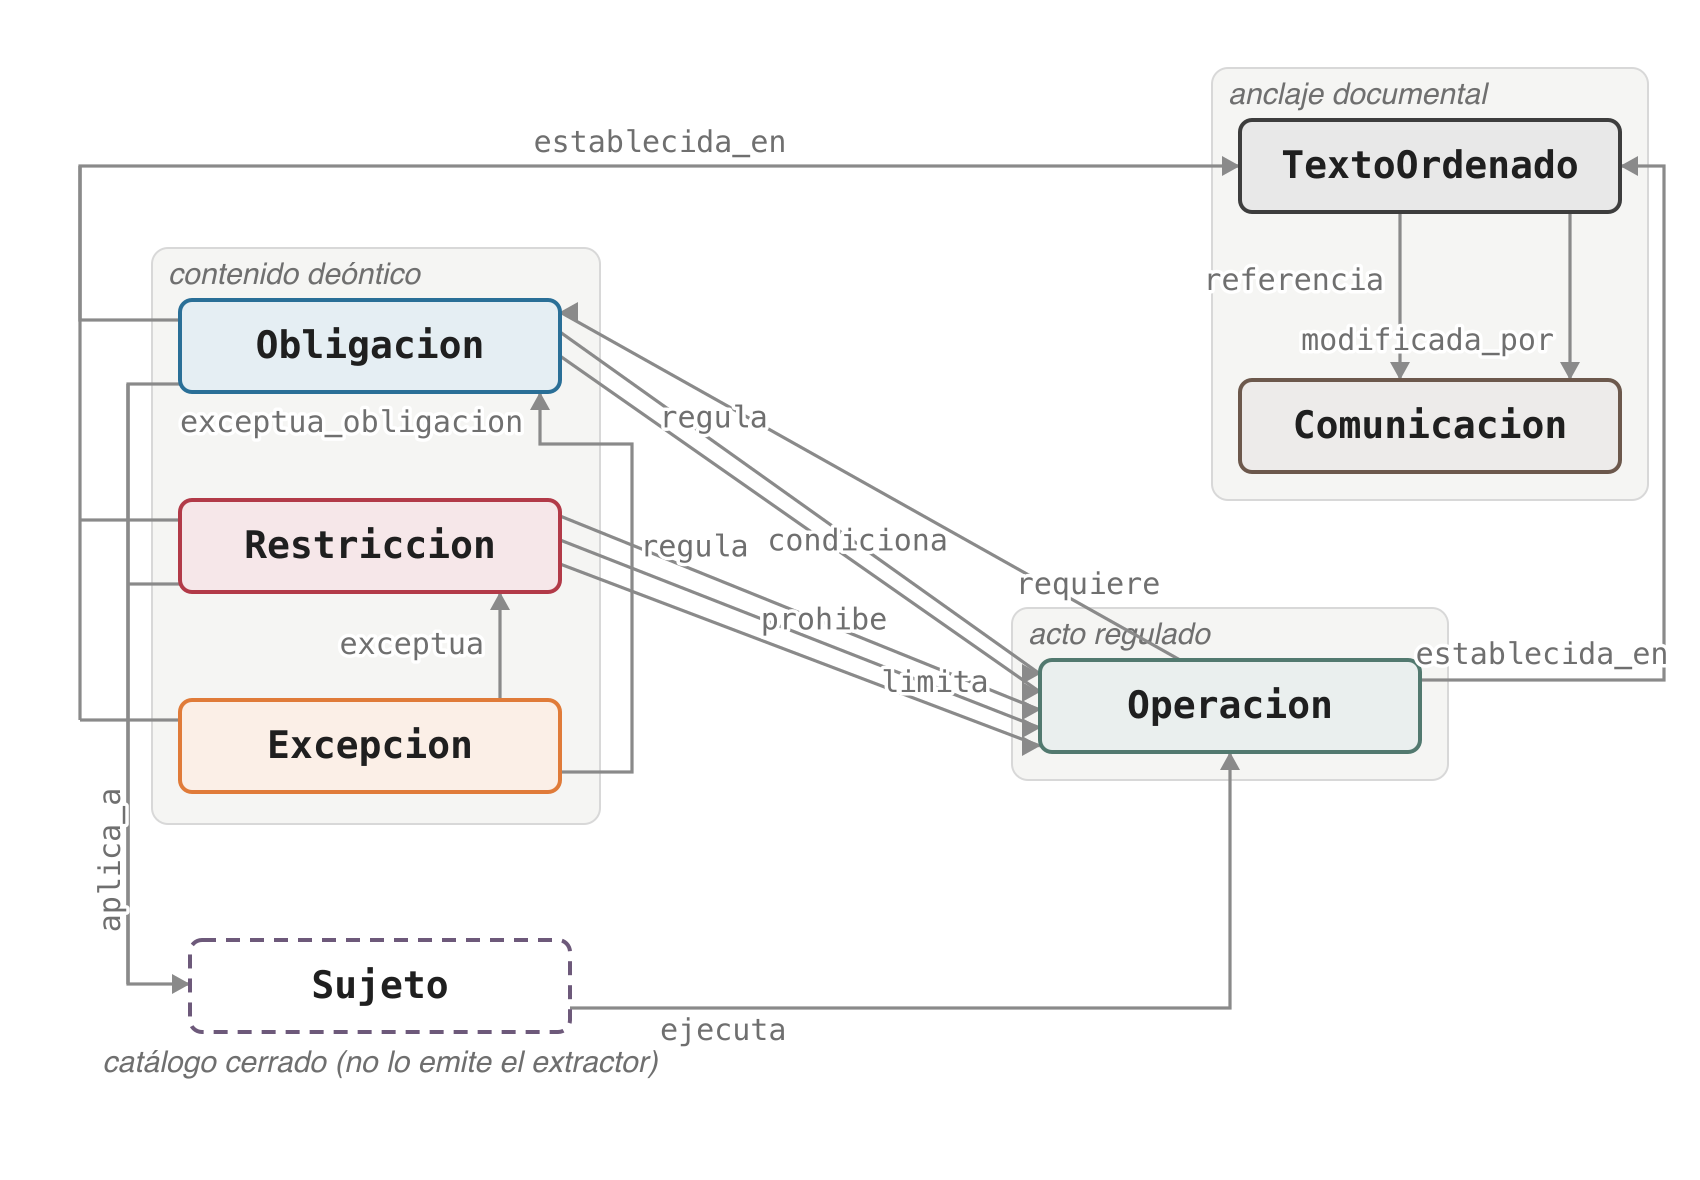
\includegraphics[width=0.85\linewidth]{figuras/figura_esquema_partida.png}
  \caption[El esquema de partida]{El esquema de partida, el que se sometió a validación. Cada caja es un tipo de entidad, agrupado según su función, y cada flecha es un par dominio-rango admitido, desde el tipo que la relación acepta como origen hacia el que acepta como destino. Las diecisiete flechas expanden las doce relaciones del esquema, porque una misma relación admite más de un par. El sujeto proviene de un catálogo cerrado y no lo emite el extractor.}
  \label{fig:esquema_partida}
\end{figure}

\section{La matriz como control}
\label{sec:matriz_control}

La matriz de dominio y rango no es documentación sino control. Al unir las extracciones en un único grafo, el ensamblado (capítulo~\ref{cap:construccion}) rechaza toda tripleta cuya firma, el par de tipos que la relación conecta, no figure en la matriz, y registra cada rechazo con la firma que intentó. El control existe porque la extracción la hace un modelo de lenguaje que, entre relaciones correctas, produce relaciones bien formadas que el esquema no admite. Sobre el conjunto de desarrollo la matriz rechazó 304 relaciones, repartidas en 29 firmas. Dos de ellas concentran 196 y son la misma forma con distinto origen, una operación o una excepción que se aplica a un sujeto, que el esquema de partida no admitía porque \texttt{aplica\_a} solo podía salir de una obligación o una restricción. Un segundo grupo de 44 tiene el mismo carácter, una excepción que exceptúa algo que no es una restricción, y las 64 restantes se dispersan en 22 firmas sin que ninguna llegue a diez relaciones. Un rechazo que se repite con esa regularidad señala un límite del esquema y no un error de la extracción, y los dos grupos entraron como insumo a la validación. La Figura~\ref{fig:figura_ejemplo_extraccion} muestra una unidad y lo que la extracción produce a partir de ella bajo este esquema.

\begin{figure}[H]
  \centering
  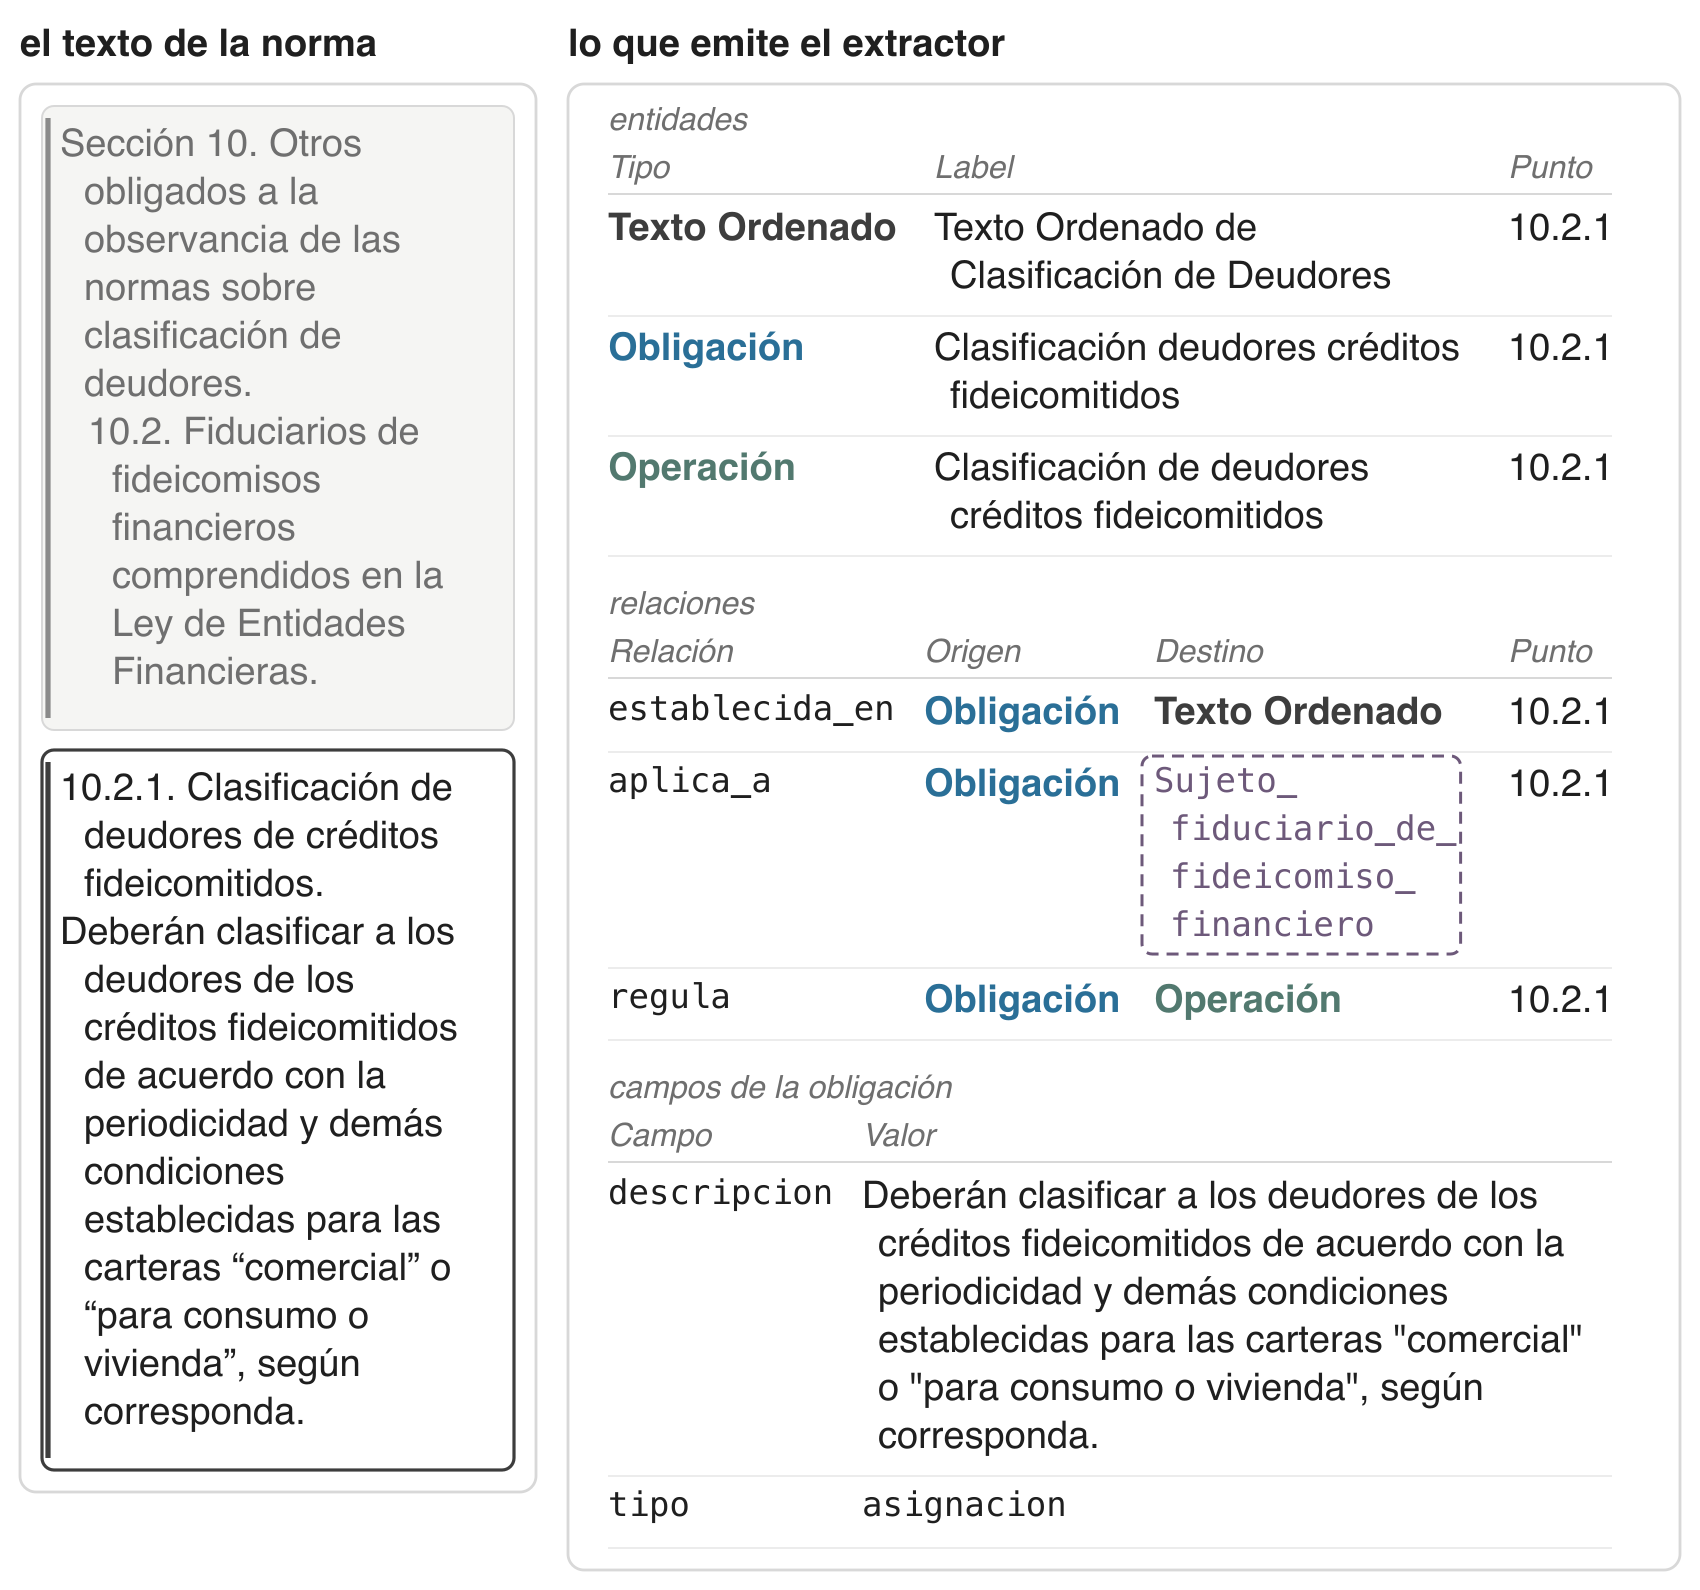
\includegraphics[width=\linewidth]{figuras/figura_ejemplo_extraccion.png}
  \caption[Una unidad de extracción y su salida]{Una unidad de extracción y lo
    que el extractor produce a partir de ella. A la izquierda, el texto
    oficial, con la cadena de encabezados que sitúa al punto en gris y el punto
    terminal, que es la unidad, en negro. A la derecha, la salida: las
    entidades y las relaciones que el esquema admite, los campos de la
    obligación y, en cada fila, el punto del que proviene. El sujeto va con
    borde punteado porque no es una entidad que el extractor emita, sino una
    entrada del catálogo elegida en un campo de la relación. Esta misma
    disposición, el texto de un lado y la salida del otro, es la ficha con la
    que se midió la cobertura en la sección~\ref{sec:cobertura}.}
  \label{fig:figura_ejemplo_extraccion}
\end{figure}

% \section{La elección del paradigma cerrado} 
\section{La comparación de estrategias de esquema} 
\label{sec:comparacion_esquemas}

El esquema de partida es cerrado en el sentido de la sección~\ref{sec:mt_kg}, y que lo sea no fue un supuesto sino el resultado de una comparación, la misma que responde por qué este trabajo no aplica tal cual un método genérico como GraphRAG (sección~\ref{sec:mt_grafos}).

Un experimento construyó cinco grafos en paralelo sobre el conjunto de desarrollo, con el mismo modelo de extracción, el mismo formato de salida con procedencia obligatoria y las mismas reglas de modelado, variando solo la estrategia de esquema. La primera siguió una guía de referencia para construir grafos con modelos de lenguaje~\cite{anthropic2026cookbook}, conservando su método completo y reemplazando solo los tipos de entidad, porque los que la guía propone pertenecen al dominio biográfico y no al regulatorio; quedó con 10 tipos y las relaciones libres. La segunda tomó un vocabulario controlado de 12 tipos y 23 relaciones, armado con los aportes de dos trabajos sobre extracción de grafos en dominios regulados~\cite{arun2025finreflect,agarwal2025ragulating}, dos estándares de representación de normativa~\cite{hoekstra2007lkif,palmirani2018akomantoso} y el modelo de procedencia del W3C~\cite{lebo2013provo}. La tercera es el esquema de partida descrito en la sección~\ref{sec:esquema_partida}, con sus 7 tipos, sus 12 relaciones y su dominio y rango estrictos. La cuarta dejó que el modelo propusiera tipos y relaciones en cada texto, sin vocabulario previo, y terminó con 858 tipos de entidad y 1.578 relaciones distintas. La quinta fijó un núcleo de 4 tipos y 5 relaciones y dejó el resto emergente.

Los cinco grafos se evaluaron por sus respuestas, con el mismo instrumento que usa el resto de este trabajo. Quien responde es el agente presentado en la sección~\ref{sec:propuesta}, un modelo de lenguaje que consulta el grafo paso a paso con tres operaciones, buscar nodos por palabras, abrir un nodo y listar sus vecinos, con un tope de 15 consultas por pregunta controlado al cierre de cada turno (sección~\ref{sec:mt_agente}). Quien califica es un modelo de lenguaje que actúa como juez y compara cada respuesta con su referencia, calibrado antes de correr contra veredictos humanos en 12 de 12 casos de prueba, con adjudicación humana de las afirmaciones que no pudo verificar contra el texto (sección~\ref{sec:mt_eval}).

Las preguntas son 23, redactadas a partir del texto fuente sin mirar los grafos y fijadas antes de correr la evaluación, y son anteriores e independientes del conjunto de evaluación del capítulo~\ref{cap:fidelidad}. De las 23, 10 piden un dato directo, 5 exigen combinar varias normas, 4 requieren seguir una restricción hasta su excepción, y 4 no tienen respuesta en el corpus y miden si el sistema se abstiene. Cada pregunta se corrió tres veces por grafo. Se midieron la corrección de las respuestas, la estabilidad entre repeticiones, la precisión de la cita (a nivel de punto, de página o ausente) y la frecuencia con que el agente agotó su límite de consultas. La Tabla~\ref{tab:cinco_estrategias} resume el resultado.
% La Tabla~\ref{tab:cinco_estrategias} resume el resultado.

\begin{table}[H]
  \centering
  \small
  \setlength{\tabcolsep}{5pt}
  \begin{tabular}{@{}lrrrrr@{}}
    \toprule
    Estrategia & \shortstack[r]{Tipos /\\relaciones} & Correctas & Estables
      & \shortstack[r]{Citas\\a punto} & \shortstack[r]{Límite\\agotado} \\
    \midrule
    Receta genérica         & 10 / libres  & 13 & 76 (83\,\%) &  0 & 33 (48\,\%) \\
    Vocabulario controlado  & 12 / 23      & 15 & 78 (85\,\%) & 12 & 26 (38\,\%) \\
    Esquema cerrado         & 7 / 12       & 16 & 86 (93\,\%) & 20 & 26 (38\,\%) \\
    Emergente               & 858 / 1.578  & 15 & 79 (86\,\%) & 14 & 34 (49\,\%) \\
    Híbrido                 & 20 / 511     & 13 & 79 (86\,\%) & 19 & 34 (49\,\%) \\
    \bottomrule
  \end{tabular}
  \caption[Comparación de cinco estrategias de esquema]{Comparación de
    cinco estrategias de esquema sobre el conjunto de desarrollo.
    Correctas sobre las 19 preguntas con respuesta; estables sobre las 92
    combinaciones pregunta-dimensión, unánimes en las tres repeticiones;
    citas a nivel de punto sobre 23 preguntas; límite agotado sobre las
    69 corridas.}
  \label{tab:cinco_estrategias}
\end{table}

El esquema cerrado obtuvo el máximo o empató en cada una de las cuatro medidas de la tabla. Fue además el único sin errores en las cuatro preguntas que siguen una restricción hasta su excepción. Por tipo de pregunta el resultado no es uniforme: en las de dato directo el esquema emergente acertó las 10 frente a 9 del cerrado, y las que combinan varias normas fueron el punto débil de las cinco estrategias, con 3 de 5 correctas para el ganador. La elección no depende de cómo se ponderen las medidas, porque el cerrado no es inferior en ninguna, y las medidas en las que las estrategias sí se separaron, la estabilidad entre repeticiones, la cita a nivel de punto y el agotamiento del límite, son las que importan para un sistema que debe responder igual cada vez y citar el punto exacto. La separación más nítida está ahí, porque la receta genérica no produjo una sola cita a nivel de punto en las 23 preguntas, de modo que sin un esquema que reserve lugar para la procedencia la respuesta no queda auditable. El conjunto de preguntas es pequeño, y esta comparación se toma como evidencia de diseño, no como resultado de la tesis.

Esa evidencia responde también a la pregunta de si este trabajo reinventa lo que un método genérico ya resuelve. Las piezas son las mismas que usa GraphRAG y ninguna es aporte de este trabajo, la extracción con un modelo de lenguaje, el grafo de propiedades, la búsqueda sobre los nodos y la navegación por las aristas. Lo que cambia es que GraphRAG es genérico por diseño, con fragmentos del mismo tamaño para cualquier colección, tipos de entidad que sirven para cualquier texto, adaptados a un dominio con ejemplos, y una capa de resúmenes redactados por el modelo para responder sobre la colección entera. La receta genérica y la estrategia emergente de la Tabla~\ref{tab:cinco_estrategias} son lo más cercano a esa forma de extraer que este trabajo corrió sobre los Textos Ordenados, por sus tipos genéricos y sus relaciones libres, y sobre este corpus la primera no produjo una sola cita a nivel de punto y la segunda quedó por debajo del esquema cerrado en estabilidad y en citas. La razón está en el corpus. Lo que la norma establece son obligaciones, restricciones y excepciones dirigidas a sujetos, escritas en puntos que remiten a otros puntos, y una respuesta sobre esta normativa vale por la cita exacta de ese punto, que un tipo genérico no reserva y que un resumen generado no puede dar. Los propios autores de GraphRAG señalan que un dominio como el derecho requiere ejemplos propios \cite{edge2024graphrag}; este trabajo da un paso más y fija el vocabulario con dominio y rango, que es lo que permite rechazar, contar y verificar, al precio de la cobertura que las secciones~\ref{sec:cobertura} y~\ref{sec:limites} miden y declaran. Por la misma razón GraphRAG tampoco sirve como término de comparación, porque mide otra cosa, la exhaustividad y la variedad de respuestas a preguntas globales y no la fidelidad a un punto ni la exactitud de la cita, y la comparación del capítulo~\ref{cap:comparacion} se hace contra la recuperación por fragmentos, que es el enfoque con el que hoy se responde sobre colecciones de documentos.

La comparación mide respuestas, y hay una razón que no depende de ellas. El entregable de este trabajo es el grafo, y un grafo con 858 tipos de entidad y 1.578 relaciones distintas no es un recurso que se pueda consultar, mantener ni actualizar. Cada consulta tendría que anticipar con qué nombre quedó escrita cada relación, y cada incorporación de normativa nueva podría traer tipos que ninguna consulta anterior contempla, de modo que el mecanismo de actualización que este trabajo propone no tendría contra qué comparar lo que llega. El vocabulario cerrado paga por adelantado el costo de decidir qué se puede decir, y a cambio le da al recurso una forma estable.

Las dos alternativas al cierre que la sección~\ref{sec:mt_kg} describe ya habían corrido en la comparación. Fijar un núcleo de tipos obligatorios y habilitar junto a él una zona de extensión libre es la estrategia híbrida de la Tabla~\ref{tab:cinco_estrategias}; no imponer vocabulario es la emergente. Ninguna de las dos superó al esquema cerrado en ninguna de las cuatro medidas. A eso se suma lo que se observó del extractor frente a un canal abierto, que es lo que una zona de extensión es en producción. El modelo no propone vocabulario nuevo sino que deforma el contenido dentro de las cajas que ya tiene, y lo hace de manera inestable. El mecanismo de descubrimiento, además, sobrecuenta: de diez propuestas revisadas a mano, siete resultaron falsos positivos; el procedimiento con que se hizo esa prueba se describe en la sección~\ref{sec:procedimiento}.

Un esquema cerrado que resulta corto se amplía por enmienda declarada, no se abre por diseño. Las ampliaciones que este trabajo evaluó, y las que efectivamente adoptó, se documentan más adelante en este capítulo.

Lo que se sometió a validación antes de escalar es el paradigma cerrado y este esquema concreto tomados juntos. Las secciones que siguen describen el catálogo del que salen los sujetos, el procedimiento con que se los puso a prueba fuera del conjunto de desarrollo, y los cambios que ese procedimiento produjo hasta el esquema congelado con el que se construye el recurso.

\section{El catálogo de sujetos}
\label{sec:catalogo}

El catálogo existe porque extraer los sujetos del texto no funcionó. Una versión anterior del esquema los extraía como un tipo de entidad más, sin control sobre la granularidad en ninguna de las dos direcciones, porque algunos se partían en tantos nodos como formas tiene el texto y el resto se apelmazaba en un nodo genérico. Un censo del grafo construido con ella midió las dos pérdidas a la vez. Ese grafo llegó a 130 nodos de sujeto, de los cuales solo trece superan las diez relaciones, y al mismo tiempo un único nodo genérico concentra 991 de las 1.464 aristas que unen una norma con su destinatario. Un grafo así registra que la norma tiene destinatario y no permite averiguar cuál. Con un catálogo el modelo no propone el sujeto sino que lo elige, y la granularidad la fija el catálogo y no el texto.

Ese catálogo no es una lista plana. Los destinatarios de la norma están a distintos niveles de generalidad, como muestra la sección~\ref{sec:docs_bcra}, y una regla dirigida a las entidades financieras alcanza también a los bancos comerciales. Una consulta que ignore esa relación devuelve media respuesta. El catálogo declara esa pertenencia, y es por eso un vocabulario con estructura.

La norma nombra a sus destinatarios de tres maneras, y el catálogo tiene una forma de entrada para cada una. Cuando nombra a un grupo, la entrada es una clase, que declara su clase madre y arma con eso el árbol. Cuando nombra a un organismo único, la entrada es una instancia, que cuelga de una clase y no tiene nada debajo. Y cuando no nombra a nadie, porque dice \enquote{las entidades comprendidas} y remite a un punto de su cabecera donde declaró una sola vez a quién se dirige, la entrada es el rol de alcance. Los grupos y organismos concretos son los de la sección~\ref{sec:docs_bcra}.

El catálogo lleva versiones propias porque crece con el corpus, mientras el esquema se mantiene fijo. Crece entre una versión y la siguiente, por decisión y no durante la extracción, de modo que el modelo nunca amplía la lista de la que elige. La versión con la que corrió la validación reúne 70 entradas, de las cuales 58 son clases, 7 instancias y 5 roles de alcance, uno por cada documento del conjunto de desarrollo. Las clases cuelgan de una raíz común y se reparten en cuatro ramas, según el sujeto sea uno de los regulados, una contraparte de la operación, un organismo público o una estructura jurídica sin personalidad propia.

Esas entradas no viven solo en el texto que se le entrega al modelo. Cada una es también un nodo del grafo, y los vínculos que declaran se escriben como 82 aristas de cuatro clases, que son 57 de \texttt{subclase\_de}, 7 de \texttt{instancia\_de}, 17 de \texttt{miembro\_de} y una de \texttt{parte\_de}, la que ata la Superintendencia al Banco Central. Ninguna de las cuatro forma parte del vocabulario que el extractor emite. Las escribe el ensamblado al cargar el catálogo, y por eso no están entre las doce relaciones que declara el esquema; llevan el rol de origen que la sección~\ref{sec:mt_kg_def} reserva para las aristas del ensamblado.

Lo que el modelo ve del catálogo no es el árbol. Recibe la lista de entradas con su etiqueta y sus alias, agrupadas por familia, y su instrucción es elegir exactamente la que el texto nombra, sin subir ni bajar por la jerarquía. Las relaciones de pertenencia no viajan en esa lista. Viven en el grafo, y son las que después permiten que una consulta por los bancos comerciales llegue a una norma dirigida a las entidades financieras. De los cinco roles de alcance el modelo ve los cinco a la vez, y solo se le dice de qué clases se compone el del documento que está procesando.

El rol y el árbol de clases se encadenan. Un punto del articulado puede exigir algo sin decir a quién, porque apunta al rol que el documento declaró una vez en su cabecera. Ese rol se compone, entre otras clases, de las entidades financieras, y los bancos comerciales cuelgan de los bancos, que cuelgan de las entidades financieras. Una consulta por los bancos comerciales llega así a una obligación que no los nombra en ningún punto, y la Figura~\ref{fig:catalogo} recorre ese camino sobre un caso real.

\begin{figure}[H]
  \centering
  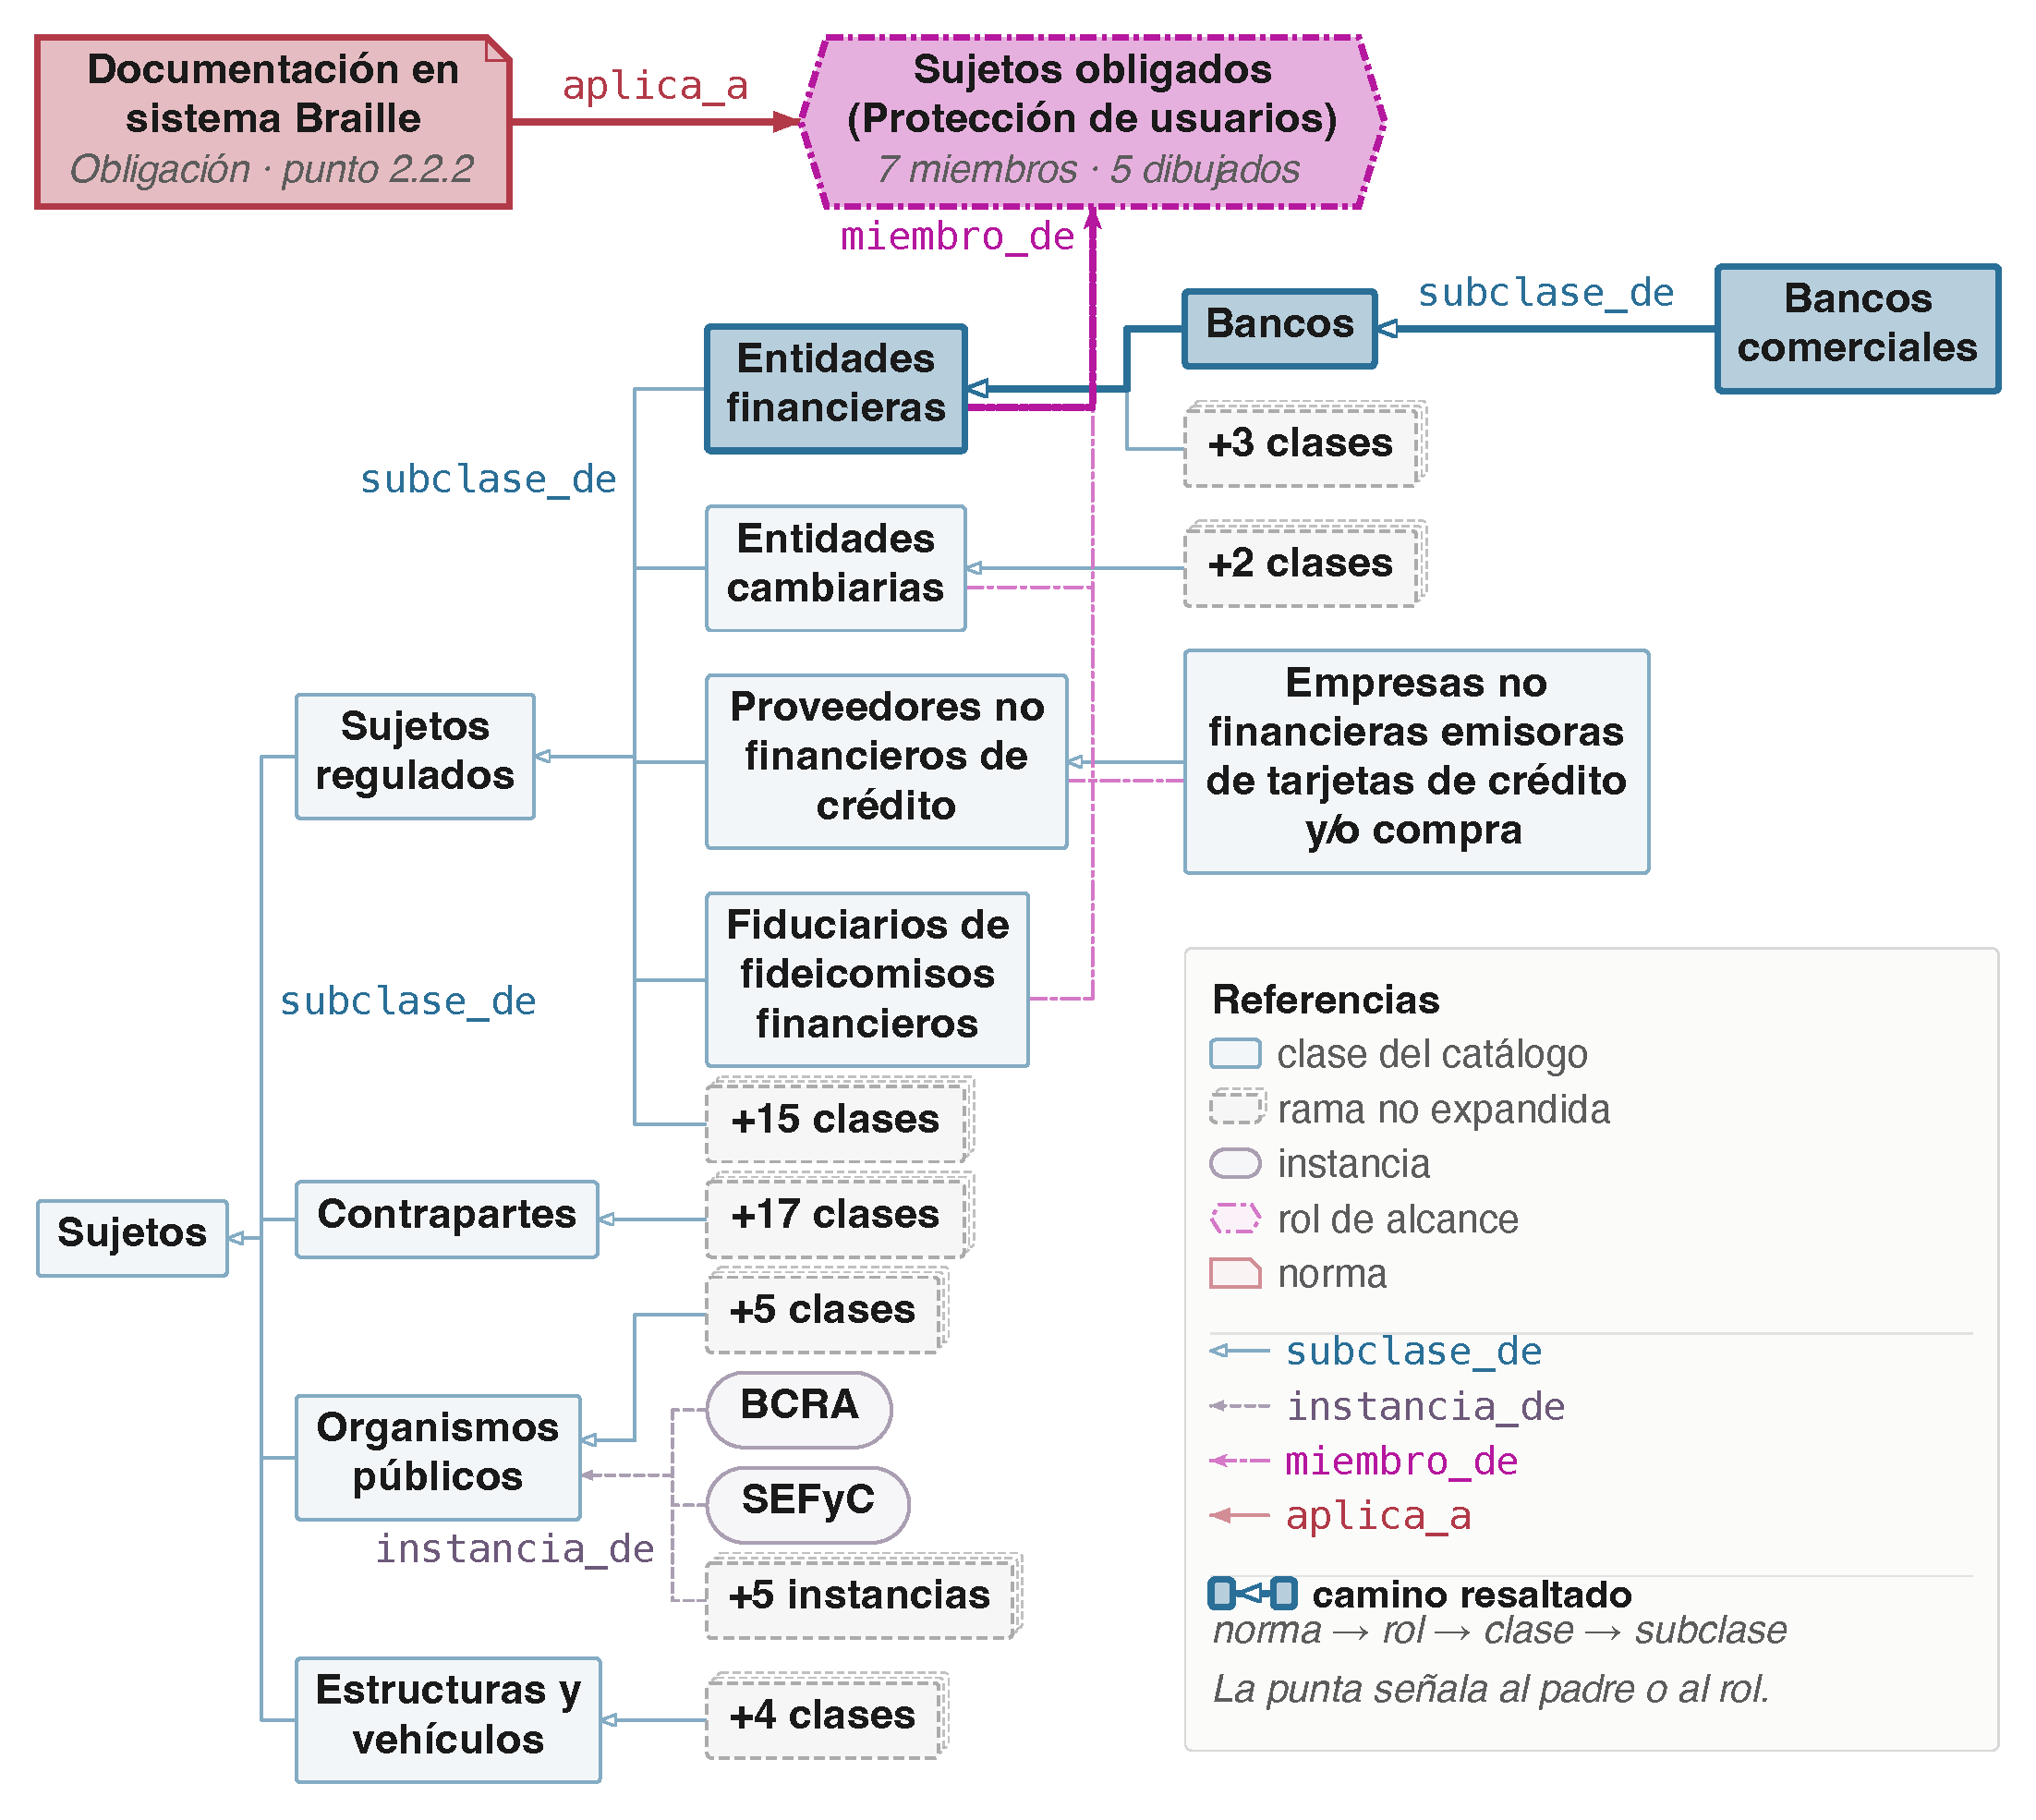
\includegraphics[width=\linewidth]{figuras/figura_catalogo_sujetos}
  \caption[El catálogo de sujetos]{El catálogo de sujetos. Las 58 clases
    forman un árbol único, y la figura dibuja doce y colapsa las 46 restantes
    en nodos que declaran cuántas contienen. En trazo grueso, el camino que esta sección recorre, el de la obligación de ofrecer documentación en
    sistema Braille (punto 2.2.2 del texto ordenado de protección de los
    usuarios) no nombra a ninguna clase, sino que apunta con
    \texttt{aplica\_a} al rol de alcance del punto 1.1.2; las clases
    declaran su pertenencia con \texttt{miembro\_de}, y de ahí el árbol
    baja hasta los bancos comerciales, que la norma nunca menciona. El rol
    tiene siete miembros y se dibujan cinco. Las instancias van por su sigla:
    BCRA, el Banco Central de la República Argentina, y SEFyC, la
    Superintendencia de Entidades Financieras y Cambiarias.}
  \label{fig:catalogo}
\end{figure}

Los cinco roles de alcance responden a un patrón de la regulación. Un Texto Ordenado fija a quién se dirige una sola vez, en un punto de su cabecera que en adelante se llama el pasaje de alcance, y lo nombra ahí con una fórmula colectiva, \enquote{entidades comprendidas}, \enquote{entidades alcanzadas}, \enquote{sujetos obligados}, a la que el resto del articulado se remite sin volver a enumerarla. Cada rol toma esa fórmula como etiqueta, registra ese punto como procedencia y declara de qué clases del catálogo se compone el colectivo, que son las 17 aristas de pertenencia ya contadas.

Lo que la Figura~\ref{fig:catalogo} muestra en un caso es el caso habitual. En el conjunto de desarrollo, ya con el catálogo en uso, hay 3.302 relaciones que unen una norma con su destinatario, y 2.766 de ellas, el 83,8\,\%, apuntan a un rol de alcance. La cifra describe al corpus antes que al recurso; los puntos del articulado casi nunca repiten a quién obligan, y el mecanismo del rol existe porque la regulación se escribe así.

Lo que el rol aporta se ve cuando falta. Los diez documentos del conjunto de validación se extrajeron sin rol propio, porque el rol solo existía para los cinco de desarrollo. El modelo no falla ni deja el sujeto vacío, y resuelve 657 de sus 727 relaciones con sujeto contra una entrada del catálogo. Lo que hace es aplanar, ya que 423 de esas relaciones terminan en la clase más amplia que encuentra, la de las entidades financieras, aunque la norma se dirigiera a un grupo más acotado. Es la misma pérdida que midió el censo de la versión anterior, más chica pero de la misma forma. Y en 18 casos el modelo elige el rol de otro documento, que sigue en su lista aunque no le corresponda.

El catálogo es cerrado pero no obligatorio. Cuando ninguna entrada corresponde, el modelo escribe el sujeto en un campo aparte, \texttt{sujeto\_propuesto}, y esa propuesta queda en cuarentena, registrada con su texto y sin ingresar al catálogo. Sobre las 4.029 relaciones con sujeto medidas en el conjunto de desarrollo y en los diez del conjunto de validación, 124 tomaron esa vía, el 3,1\,\%. La tasa no es pareja entre los dos conjuntos. En desarrollo, donde cada documento tiene su rol declarado, es del 1,6\,\%, y en los diez de validación, sin rol propio, sube al 9,6\,\%.

Ese campo existe porque la alternativa borra el problema. Forzar al modelo a elegir la entrada más parecida cuando ninguna corresponde fabricaría un sujeto que la norma no nombra, y lo haría sin dejar rastro. En cambio, el desajuste entre el catálogo y el texto queda escrito y se puede contar, y es la evidencia con la que se decide si el catálogo debe crecer.

Las 124 propuestas son esa evidencia, y podían significar que al catálogo le faltaban entradas. Un mismo sujeto aparece escrito de maneras distintas, así que primero se agruparon por el sustantivo que las encabeza, con un procedimiento mecánico y sin modelo de lenguaje. El corte para que un grupo entrara al catálogo se fijó antes de mirar la distribución, y exige aparecer en al menos 20 unidades de extracción, en al menos 5 documentos y en al menos 2 de los diez de validación. Fijarlo de antemano evita elegir después el umbral que da el resultado esperado. Ningún grupo lo alcanzó, ni lo alcanza con los umbrales más bajos que la propia medición reporta como control.

El catálogo con el que se validó el esquema queda entonces en esas 70 entradas. Volvió a crecer al incorporar el resto del corpus, y el capítulo~\ref{cap:construccion} trata esa extensión, lo que deja sin cubrir y qué documentos del conjunto de validación intervinieron en ella.

\section{El procedimiento de validación}
\label{sec:procedimiento}

El esquema y el catálogo se pusieron a prueba sobre los diez documentos del conjunto de validación, y la primera pregunta de esa prueba no fue cuánto acierta el extractor sino qué contenido de la norma no tiene lugar en el vocabulario. Un esquema cerrado no puede responderla por sí solo, porque aquello que no admite no produce salida y por lo tanto no deja rastro que contar. Hacía falta un instrumento que le diera al extractor un lugar donde escribir lo que no entra. Se ensayaron dos y ninguno pasó su control, pero el modo en que fallaron dice algo sobre el extractor que la medición posterior confirmó.

El primero fue el canal abierto. Son dos campos adicionales, uno para el tipo de entidad y otro para el tipo de relación, con la misma forma que el campo aparte del sujeto ya descrito. El modelo sigue eligiendo dentro del vocabulario cerrado, y cuando un contenido normativo claro no cabe en ninguna caja lo escribe en esos campos en lugar de forzarlo o de callarlo.

El catálogo de sujetos ya tenía un campo de ese tipo. El modelo lo usa cuando ninguna entrada corresponde, y sobre el conjunto de desarrollo lo emitió 56 veces, con 39 expresiones distintas, de las que 54 sobrevivieron a la validación y son las que contó la sección anterior. Los tipos de entidad y de relación no tenían nada equivalente, de modo que sobre ellos no había manera de saber cuánto quedaba afuera.

Antes de usar el canal para medir nada hubo que probar que funciona. Si la medición diera cero, ese cero admitiría dos lecturas incompatibles, que el esquema alcanza para todo y que el modelo nunca escribe en el canal, y ninguna medición posterior las separa. Por eso quedó escrito, antes de la primera corrida, que sin un control aprobado ningún resultado sería admisible, ni un cero ni un número distinto de cero. Se corrieron cuatro, y la Tabla~\ref{tab:controles} los reúne con su material, lo que cada uno exigía y lo que produjo.

\begin{table}[H]
  \centering
  \small
  \setlength{\tabcolsep}{5pt}
  \renewcommand{\arraystretch}{1.15}
  \begin{tabularx}{\textwidth}{@{}l >{\raggedright\arraybackslash}X c c@{}}
    \toprule
    Control & Grupo & Se exigía & Se obtuvo \\
    \midrule
    Primero & 20 unidades con omisión ya declarada & $\geq$10 & 0 \\
            & 10 con una relación rechazada por la matriz & $\geq$7 & 3 \\
            & 10 limpias & $\leq$1 & 0 \\
    \addlinespace
    Segundo & 10 unidades dopadas & $\geq$7 & 0 \\
            & 10 limpias & $\leq$1 & 0 \\
    \addlinespace
    Tercero & 10 dopadas, con las dos frases que compiten con el canal reemplazadas & $\geq$7 & 0 \\
            & 10 limpias & $\leq$1 & 0 \\
    \addlinespace
    Cuarto & 10 dopadas, leídas por la consulta separada & $\geq$7 & 9 \\
           & 10 limpias & $\leq$1 & 7 \\
    \bottomrule
  \end{tabularx}
  \caption[Los cuatro controles]{Los cuatro controles corridos antes de admitir cualquier medición automática de lo que el esquema no cubre. Los tres primeros prueban el canal abierto y el cuarto calibra la consulta separada.
    Los grupos donde el canal tenía que escribir llevan un piso y los
    grupos limpios un techo. Cada control se corrió solo después de que
    el anterior fallara de una forma determinada. Los dos primeros grupos del primer control resultaron mal construidos, por las razones que la sección explica, y sus cifras no miden lo que el control se proponía medir. El grupo limpio cambia
    de papel en el cuarto: en los tres primeros acota cuántas veces el
    canal escribe donde no corresponde, y en el cuarto cuántos hallazgos
    falsos produce la lectura. El grupo de diez unidades limpias es el mismo en los cuatro controles.}
  \label{tab:controles}
\end{table}

El primer control tomó 40 unidades ya extraídas del conjunto de desarrollo y las repartió en tres grupos. Antes de correrlo quedó escrito cuántas unidades de cada grupo tenían que usar el canal para darlo por aprobado. En veinte el extractor ya había anotado, en un campo aparte, que dejaba contenido sin extraer, de modo que son el lugar donde el canal tendría que escribir, y se exigían al menos diez. Otras diez habían producido relaciones que la matriz de dominio y rango rechazó, señal de que el modelo intentó decir algo que el esquema no admite, y se exigían siete. Las diez últimas estaban limpias, sin nada que reportar, y servían para detectar lo contrario, que el canal escriba cuando no corresponde; ahí se admitía como máximo una.

El canal escribió muy por debajo de lo exigido en los dos grupos donde tenía que escribir. En el grupo limpio, donde no tenía que escribir, no escribió ninguna vez, y ese fue el único umbral cumplido. Un grupo limpio sirve para descartar que el canal se dispare de más, no para mostrar que se dispare cuando corresponde. El control no quedó aprobado.

El control falló, pero antes de concluir nada sobre el canal hubo que revisar el control mismo, y dos de sus tres grupos estaban mal construidos. Las instrucciones del extractor le piden omitir lo que no encaja antes de que llegue a elegir un tipo, así que en el grupo de las veinte unidades con omisión ya declarada anotar la omisión y no escribir en el canal son la misma conducta y no dos. Ese grupo terminaba midiendo si la instrucción de omitir es estable, y lo es: el modelo volvió a anotar la misma omisión en 19 de las 20 unidades.

El grupo de las diez unidades con una relación rechazada tenía otro problema. Esas unidades se eligieron porque en una corrida anterior el modelo había producido en ellas relaciones que la matriz rechazó, y el modelo no repite exactamente su conducta entre corridas. Al volver a correrlas esos rechazos iban a bajar por sí solos, hubiera canal abierto o no, de modo que el número de ese grupo no diría nada sobre lo que se quería probar. Hacía falta un control cuyo resultado esperado no dependiera de nada que el modelo hubiera hecho antes.

El control siguiente se construyó plantando el problema. A diez unidades reales del conjunto de desarrollo se les añadió, a cada una, exactamente una cláusula normativa en prosa, redactada para no caber en el esquema y verosímil como texto del BCRA. Cinco piden un tipo de entidad que el vocabulario no tiene, como una sanción de multa o una facultad discrecional del supervisor, y las otras cinco una relación que la matriz no admite. Esas son las unidades dopadas. El contenido plantado se aprobó antes de la corrida, y ni las cláusulas ni sus conceptos aparecen en las instrucciones del extractor ni en ningún ejemplo. Junto con el material se corrigió también la descripción del campo en el esquema de la herramienta, que era uno de los textos del prompt que competían con el canal, de modo que entre el primer control y este cambiaron dos cosas.

El canal no se usó una sola vez, y el registro de la corrida dice qué ocurrió en lugar de eso. El modelo leyó las diez cláusulas plantadas y las extrajo todas dentro del esquema, sin declarar una sola omisión.

Ese silencio llama la atención porque el mismo mecanismo funciona para los sujetos, y con la misma instrucción. Tanto el campo del sujeto como los dos del canal piden explícitamente proponer antes que forzar. Lo que los distingue es lo que tienen enfrente. El canal se ofrece dentro de un texto que encabeza la lista declarando que los tipos son seis y ningún otro, y que entre sus reglas no negociables pide no inventar y preferir no extraer antes que forzar una caja. El campo de sujeto no compite con nada de eso.

Se reemplazaron dos de esas frases, solo en el modo de medición, dejando idénticas las diez unidades dopadas, los umbrales y el grupo de unidades limpias, de modo que entre una corrida y la otra cambiara una sola cosa. El resultado no cambió, y las 20 unidades comparadas una a una contra la corrida anterior no registran una sola diferencia. El precio de ese control quedó declarado: con los cierres neutralizados el modo de medición deja de ser el de producción más un agregado, y pasa a ser un prompt distinto. Antes de esa corrida estaba fijado que sería la última: si volvía a dar cero, el canal quedaba declarado inviable y no habría un tercer ajuste del lenguaje. Fijarlo de antemano evita seguir retocando las instrucciones hasta que el modelo escriba en el canal. Neutralizados los cierres, la asimetría entre los dos campos queda sin explicación medida.

El segundo instrumento es la consulta separada. En lugar de pedirle al extractor que extraiga y de paso avise, se le pregunta a un modelo, en una llamada aparte y sin pedirle que extraiga nada, qué contenido normativo de la unidad no encaja en el esquema. Antes de censar el corpus con ella se la calibró contra la misma vara, las diez unidades dopadas y las diez limpias, con los mismos umbrales, y esa calibración es el cuarto control de la tabla.

Sobre las dopadas el instrumento funciona. Detecta 9 de las 10 cláusulas plantadas, cita el pasaje y explica por qué no encaja, y en ningún caso confunde un tipo faltante con una relación faltante. Sobre las diez unidades limpias señala contenido fuera del esquema en 7, y en las 7 lo señalado es contenido que el esquema sí representa, como restricciones cualitativas, excepciones y deberes de informar. En el grupo limpio se admitía como máximo una detección, y hubo siete.

Los dos instrumentos fallaron por razones opuestas. El canal abierto no declara nunca, ni siquiera cuando el contenido plantado no cabe de ninguna manera, y la consulta separada declara de más, porque señala como faltante contenido que el esquema sí representa. La vía del censo automático quedó cerrada por una regla propia de un solo intento, declarada antes de la calibración con la misma forma que la del canal, y la cobertura se midió leyendo las unidades una por una. La Figura~\ref{fig:controles} recorre los cuatro controles en el orden en que se corrieron, y sobre cada flecha lleva el motivo por el que después de uno hubo otro.

\begin{figure}[H]
  \centering
  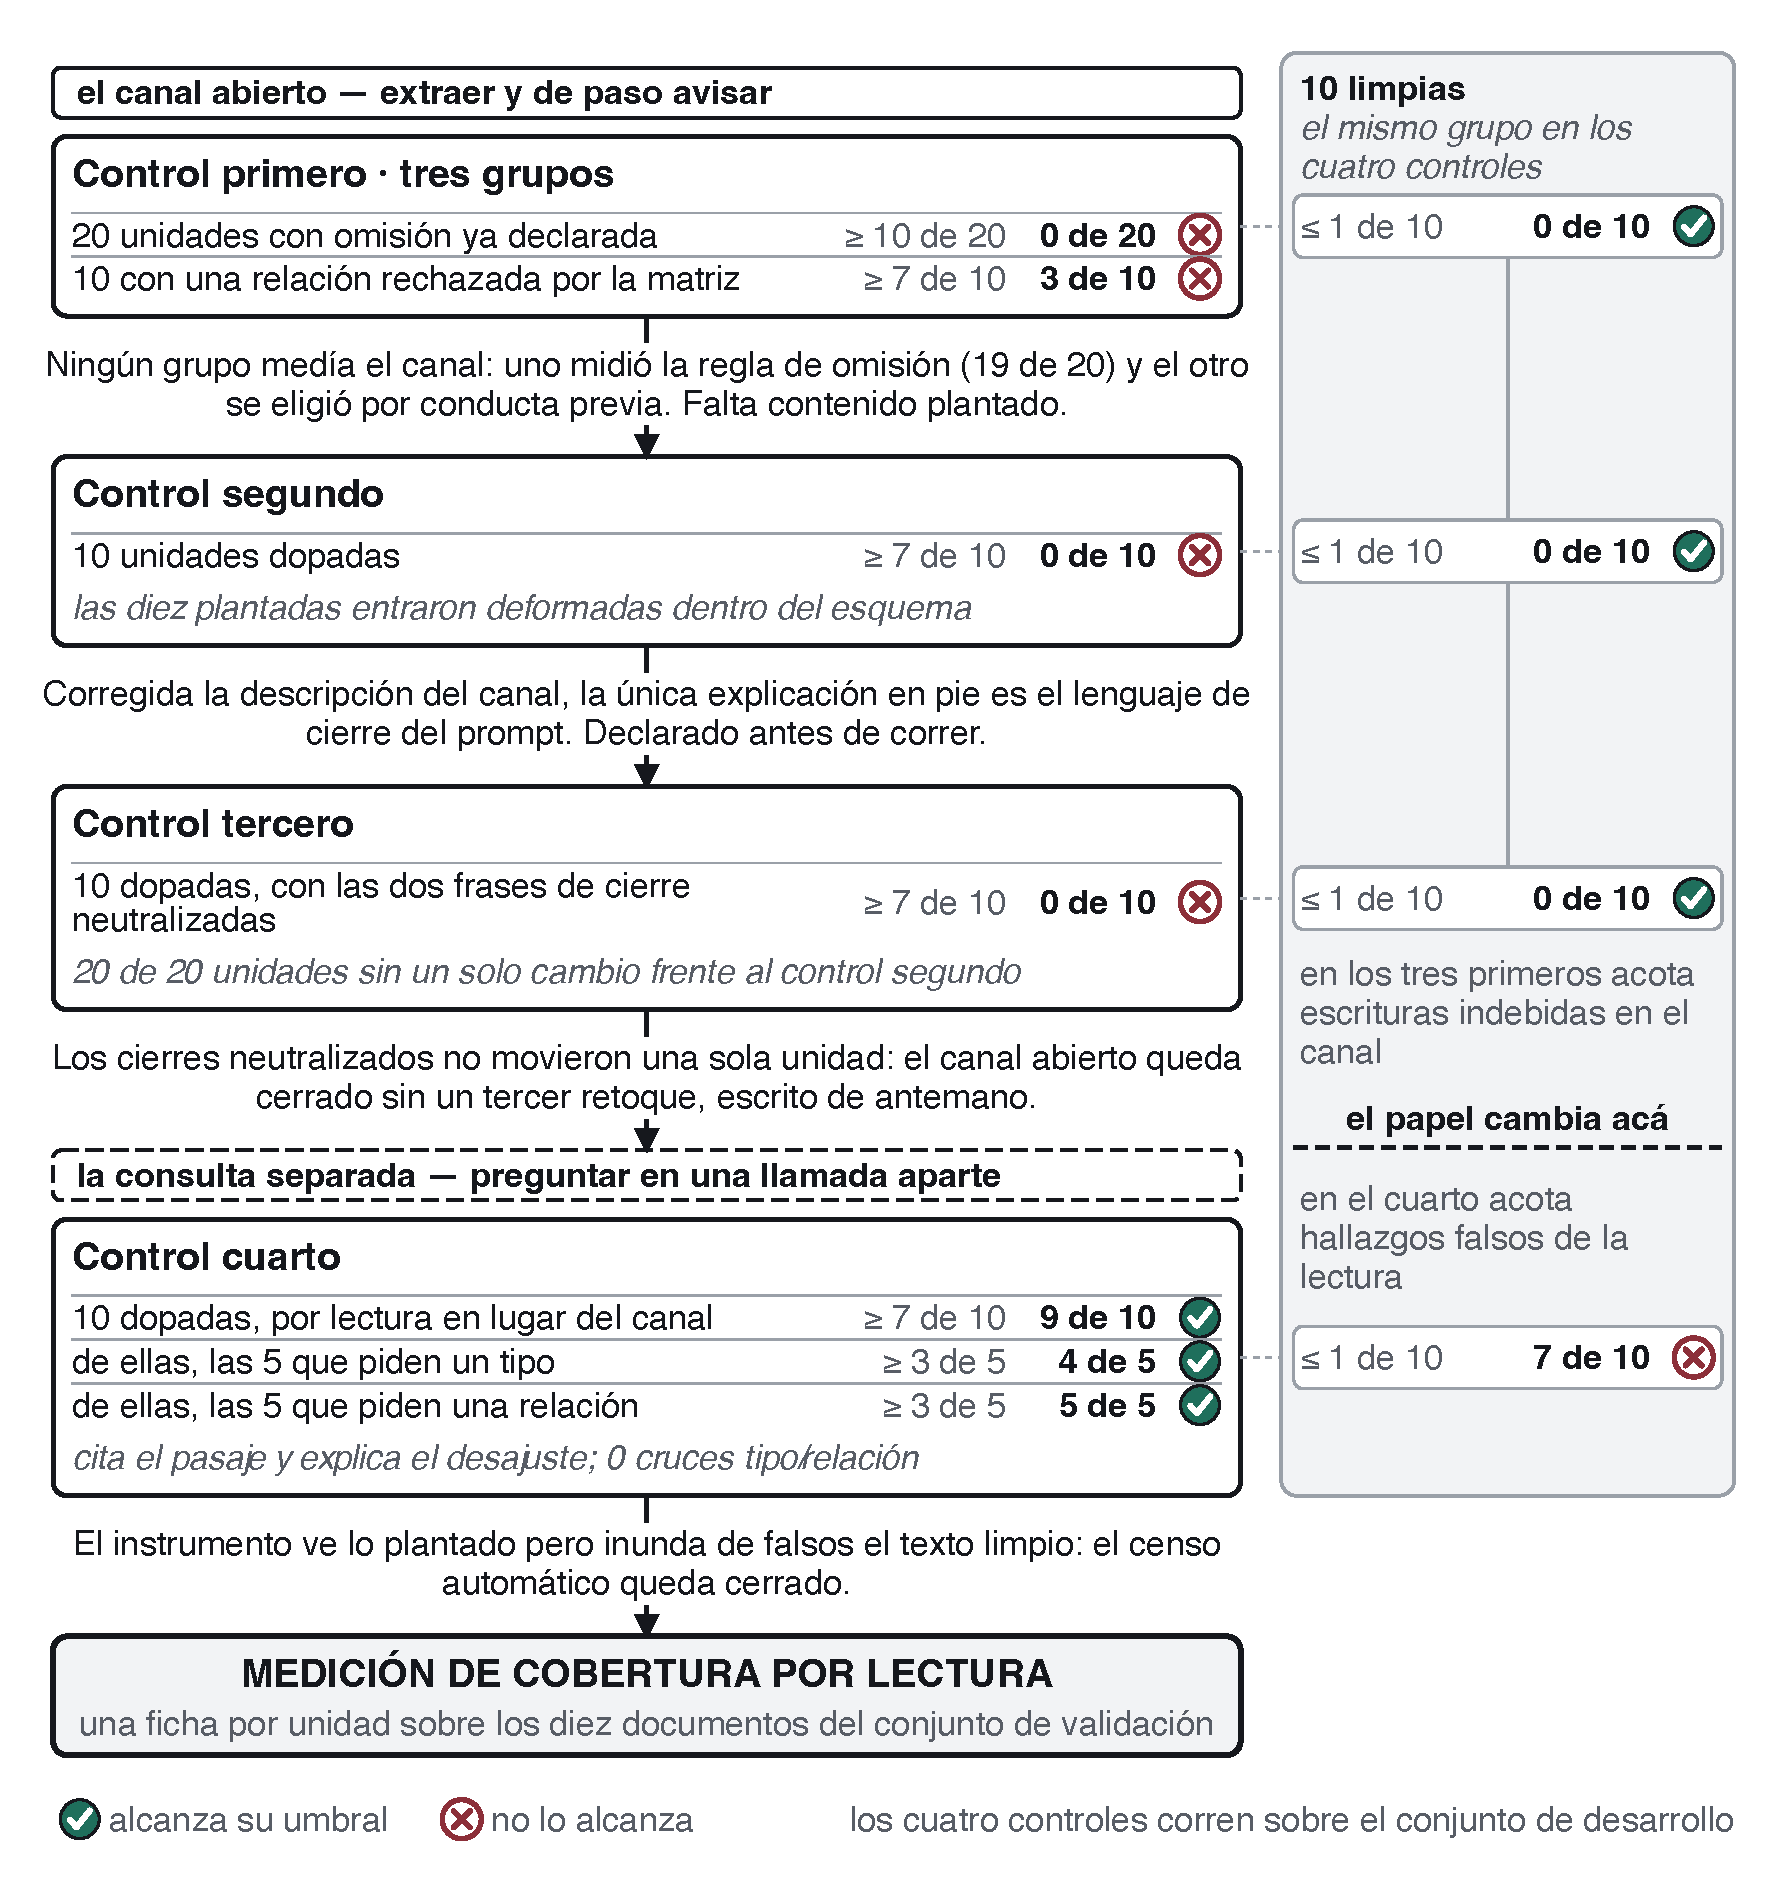
\includegraphics[width=\linewidth]{figuras/figura_controles}
  \caption[Los cuatro controles del canal]{Los cuatro controles, en el
    orden en que se corrieron. Sobre cada flecha va el motivo por el que
    hubo un control más, porque ninguno se corrió sin que el anterior
    fallara de una forma determinada. Los tres primeros prueban el canal
    abierto y el cuarto cambia de instrumento. El grupo de diez unidades
    limpias corre por la columna de la derecha y cambia de papel entre el
    tercer control y el cuarto, donde pasa de acotar escrituras indebidas
    en el canal a acotar hallazgos falsos de la lectura.}
  \label{fig:controles}
\end{figure}

La escalera dejó, de todos modos, una observación sobre el extractor. El contenido que no cabe en el vocabulario no desaparece de la salida, ingresa forzado en las cajas que hay.

La consulta separada dejó otra. Entre lo que señaló sobre texto de producción hubo cuatro detecciones ciertas, dos de ellas facultades discrecionales del supervisor, que es la categoría plantada como hipótesis en una de las unidades dopadas. La medición que sigue volvió a encontrarla por lectura sobre texto real.

\section{La medición de cobertura sobre el conjunto de validación}
\label{sec:cobertura}

Cerradas las dos vías automáticas, la cobertura del esquema se midió leyendo unidad por unidad. El instrumento es una ficha por unidad como la de la Figura~\ref{fig:figura_ejemplo_extraccion}, con el texto oficial de la norma de un lado, junto con la cadena de encabezados que la contiene, y del otro lo que el extractor produjo a partir de él. Sobre cada ficha se responden tres preguntas: si el contenido normativo está representado, qué deformación hay cuando la hay, y qué quedó sin extraer.

El material son los diez documentos del conjunto de validación, 762 unidades de extracción sobre 254 páginas, y dos condiciones de esa extracción gobiernan cómo se leen las cifras. La primera es que corrió solo la etapa del extractor, sin el verificador que después compara lo extraído contra el texto del que salió y vuelve a extraer la unidad cuando encuentra contenido sin representar. El pre-registro selló por eso que el conteo de omisiones de esta medición es una cota superior del que daría el proceso completo. Esa cota alcanza a las omisiones y no al resto de las cifras, y no es estricta, porque la re-extracción reemplaza a la primera pasada en lugar de sumarse a ella y puede perder contenido que la primera sí había representado. La segunda condición es que esos documentos se extrajeron sin rol de alcance propio. Sin esos roles el campo aparte del sujeto se dispara por una carencia conocida de esta corrida y no por un hueco del vocabulario, y sus disparos no permiten distinguir una causa de la otra, de modo que la cobertura de los sujetos queda fuera de esta medición y ninguna de las cifras que siguen habla de ella.

La lectura y la adjudicación de las 75 fichas las hizo la autora de este trabajo, en tandas de diez a quince y con una regla de adjudicación sellada antes de empezar. Las fichas vienen de dos muestras. Treinta y ocho salieron de un sorteo estratificado por documento, en el que a cada uno le tocaron tantas fichas como le correspondían por su tamaño, con un piso de dos para que ninguno quedara sin representación, y dentro de cada documento las unidades se sortearon con semilla registrada. Esa es la muestra que generaliza, y la única sobre la que se calculan intervalos.

La muestra azarosa dice con qué frecuencia aparece cada problema, pero un problema poco frecuente puede no salir sorteado ni una vez en 38 fichas. Por eso se armó una segunda muestra de 37 fichas, elegida a propósito entre las unidades que más probablemente tuvieran algo mal. Para encontrarlas sin leerlas se computaron cuatro señales sobre la extracción completa, y cada una es un síntoma mecánico de que el extractor forzó contenido en una caja que no le correspondía. Una relación escrita como si fuera una entidad indica que el predicado que hacía falta no existía. El campo de tipo resuelto con el valor genérico indica que ningún valor específico servía. Una entidad que no quedó conectada con ninguna otra, más allá de la norma donde está escrita, indica que su vínculo no tenía cómo expresarse. Y una unidad con una cantidad de elementos muy fuera de lo común indica que se descompuso mal.

Cada señal marca muchas más unidades de las que se pueden leer, así que una regla fijada antes de mirar ninguna decide cuáles de las marcadas entran a las 37, para que no se elijan después las que se ven más jugosas. Esa regla, tal como se selló, no funcionó, y el defecto y su corrección se declaran más abajo con el resto de los desvíos. Lo que esta muestra aporta es encontrar lo que el azar puede no ver, y lo que no puede dar son frecuencias: como se eligió por sospechosa, tiene más problemas que el promedio por construcción, se reporta aparte y sin intervalos, y por criterio sellado de antemano no alcanza por sí sola para incorporar ninguna categoría nueva al esquema.

La lectura se rodeó de tres precauciones. La ficha muestra la extracción cruda del modelo y no la salida del validador, porque los rechazos del validador por sujeto harían visible la falta del rol de alcance, y por el mismo motivo esa falta quedó excluida de las cuatro señales mecánicas. Las fichas no dicen de qué muestra provienen y se leen en un orden aleatorizado con semilla registrada, de modo que ninguna se lee sabiendo que fue elegida por sospechosa. Y la duda es una categoría propia en las tres preguntas, así que una ficha difícil se marca como dudosa en lugar de forzar una respuesta, y no infla ni el resultado que dice que el esquema alcanza ni el que dice que no.

Sobre las 38 fichas azarosas, 10 unidades quedaron representadas por completo, 23 de forma parcial y 5 no quedaron representadas, y la Tabla~\ref{tab:cobertura} reúne esas cifras junto con las de deformación y omisión. En tres de cada cuatro unidades el contenido normativo no queda representado por completo, y en algo más de una de cada diez no queda representado en absoluto.

\begin{table}[H]
  \centering
  \small
  \setlength{\tabcolsep}{5pt}
  \renewcommand{\arraystretch}{1.15}
  \begin{tabularx}{\textwidth}{@{}>{\raggedright\arraybackslash}X c c c@{}}
    \toprule
     & Fichas & \% & IC 95\,\% \\
    \midrule
    \multicolumn{4}{@{}l}{\itshape Representación del contenido normativo} \\
    Parcial o nula & 28 de 38 & 74 & 58--85 \\
    Nula & 5 de 38 & 13 & 6--27 \\
    \addlinespace
    \multicolumn{4}{@{}l}{\itshape Deformación del contenido representado} \\
    Cualquier patrón & 16 de 38 & 42 & 28--58 \\
    Re-tipado semántico & 8 de 38 & 21 & 11--36 \\
    Potestades y facultades & 6 de 38 & 16 & 7--30 \\
    \addlinespace
    \multicolumn{4}{@{}l}{\itshape Contenido omitido} \\
    Remisión normativa sin arista posible & 11 de 38 & 29 & 17--45 \\
    \bottomrule
  \end{tabularx}
  \caption[Cobertura del esquema sobre la muestra azarosa]{Resultados sobre las
    38 fichas de la muestra azarosa del conjunto de validación. Los intervalos son
    de Wilson al 95\,\% \cite{wilson1927}, elegido en lugar del intervalo
    normal porque con muestras de este tamaño y proporciones cercanas a los
    extremos el normal cubre menos de lo que declara \cite{brown2001}. Valen
    solo para esta muestra, que es la única sorteada. La etapa de verificación
    del proceso completo no corrió, de modo que las cifras describen la salida
    del extractor y no la del recurso final.}
  \label{tab:cobertura}
\end{table}

La deformación se contó aparte de la omisión, porque son fallas distintas. Una unidad puede estar entera en el grafo y estar mal puesta, que es la conducta que los controles del canal ya habían dejado a la vista. El patrón más frecuente es el re-tipado semántico, contenido puesto en una caja que no le corresponde, y aparece en los diez documentos del conjunto de validación. Le siguen las potestades y facultades, que el esquema no tiene cómo representar porque no son deber positivo, ni prohibición, ni excepción, ni acto regulado.

La muestra dirigida encontró más deformación que el azar, 21 de sus 37 fichas contra 16 de 38, de modo que las cuatro señales mecánicas hicieron lo que se esperaba de ellas. Aportó además el único registro de un patrón que la azarosa no vio ninguna vez, el de los hechos con valor aplastados, umbrales y plazos de los que depende que la norma se aplique y que quedan escritos dentro de la prosa de la descripción en lugar de un campo propio, en 4 fichas de 4 documentos distintos. Por el criterio sellado de antemano, esa evidencia no alcanza por sí sola para incorporar el patrón al esquema.

Las omisiones no tenían categorías predefinidas. Quien leía anotaba con etiquetas libres lo que faltaba, y esas 15 etiquetas crudas se agruparon después en trece familias, con el criterio de fusión declarado caso por caso. La familia más frecuente es la remisión normativa sin arista posible, presente en 9 de los diez documentos.

Cada familia quedó anotada con su destino, tomado de las notas que la lectura dejó en cada ficha y no decidido después de ver los resultados agregados. Un destino posible es que la resuelva el armado del grafo, otro que exija ampliar el esquema, y otro que sea deuda del extractor y no del vocabulario. Ese destino dice qué haría falta para cubrir una familia, no si se la va a cubrir. Eso lo decide un criterio aparte, sellado antes de leer, según el cual una familia queda como candidata a ampliar el esquema si aparece en al menos 3 de las 38 fichas azarosas o en al menos 3 de los diez documentos contando las dos muestras, y queda como residuo documentado si no alcanza ninguna de las dos vías. La muestra dirigida puede corroborar una candidata y nunca promoverla por sí sola. La decisión se toma en la sección siguiente.

El procedimiento tuvo cuatro desvíos, los cuatro declarados con su tratamiento. El primero ocurrió antes de leer una sola ficha. La regla de selección de la muestra dirigida ordenaba las unidades marcadas por su identificador y tomaba las primeras de la lista, y como el identificador de una unidad empieza por el de su documento, ordenar por identificador equivale a agrupar por documento. El documento que va primero en el alfabeto encabezaba las cuatro listas con 70 marcas sobre 44 unidades distintas, para 37 lugares, y las 37 fichas quedaron compuestas por 36 unidades de ese único documento. El defecto se detectó antes de leer la primera ficha, y la corrección quedó asentada por escrito con la regla anterior y la que la reemplaza, que alterna entre las cuatro señales y entre los documentos en lugar de vaciar una lista antes de pasar a la siguiente. La muestra azarosa no se tocó, porque nunca dependió de esta regla, y la dirigida que efectivamente se leyó quedó repartida entre los diez documentos, con un máximo de cinco fichas por documento.

El segundo es que diez fichas no se leyeron a ciegas, porque la decisión se tomó con la lectura de un asistente automático sobre la misma unidad a la vista. El desvío quedó anotado ficha por ficha durante la propia lectura, pero la regla que trata a esas diez como contaminadas se fijó después del hecho, y por eso el recómputo se reporta junto a las cifras originales y no en su lugar. Cuatro de las diez pertenecen a la muestra azarosa, y recomputadas las 34 restantes las tres cifras de cabecera de la Tabla~\ref{tab:cobertura} pasan del 74 al 71\,\% en representación parcial o nula, del 13 al 12\,\% en representación nula y del 42 al 38\,\% en deformación. Ninguna se mueve lo suficiente como para cambiar una conclusión.

Los dos últimos son fallas del instrumento de lectura. Uno truncó 36 campos de análisis complementario por el límite de línea de la terminal, sin afectar las marcas de las tres preguntas ni las citas textuales, que están completas en las 75 fichas. El otro es una colisión de teclas que hacía imposible registrar el patrón de las potestades, detectada en la ficha 15, la primera donde hizo falta marcarlo, de modo que la ventana en riesgo son las fichas 1 a 14. En esas catorce hay una sola marca que pudo haberse perdido, y se adjudicó que no lo era porque la nota que la acompaña explica la duda por otro motivo. En el peor caso las potestades pasarían de seis fichas azarosas a siete, y ninguna otra cifra se mueve.

Las limitaciones de la medición están en su tamaño, en su material y en quién leyó. Con 38 fichas azarosas los intervalos son anchos, de modo que la muestra dimensiona magnitudes gruesas y no diferencias finas, y los estratos por documento dan cobertura del corpus y no comparación entre documentos. Y las 75 fichas las leyó una sola persona, que es además la autora del esquema que se estaba midiendo, de modo que el juicio no es independiente del interés en el resultado. Contra eso operan las tres precauciones ya descritas, y ninguna de las tres reemplaza a un segundo lector.

Hay una limitación más, de otra clase. Los diez documentos no intervinieron en el esquema de partida, y por eso esta medición es una prueba legítima de ese esquema. Pero los cambios que la medición produzca van a salir de ellos, así que el esquema resultante ya habrá visto este material. Evaluar ese esquema resultante exige documentos que no hayan participado de nada de esto, y la sección~\ref{sec:limites} vuelve sobre ese punto con el material que el mismo sorteo reservó para eso.

\section{La enmienda del esquema}

La medición produjo dos clases de resultado, una por cada una de las dos últimas preguntas de la ficha: los patrones de deformación, que clasifican lo que quedó representado de forma incorrecta, y las familias de omisión, que clasifican lo que quedó sin extraer. Son dos clasificaciones paralelas y ninguna está contenida en la otra. El criterio sellado antes de leer decide sobre unas y otras. Esta sección lo aplica, establece qué haría falta para cubrir cada resultado promovido, propone con eso los cambios al esquema, y los somete a una prueba que decide cuáles quedan. Entra al esquema lo que el criterio promovió y cuyo remedio es vocabulario nuevo, porque no todo lo promovido lo pide, y lo demás queda como residuo documentado o como límite conocido del esquema.

\subsubsection*{Los patrones de deformación}

El criterio se aplica primero a los patrones. Son seis, de una lista cerrada fijada antes de leer. Dos lo superan por las dos vías a la vez, la de al menos tres fichas azarosas y la de al menos tres documentos. El re-tipado semántico aparece en ocho fichas azarosas y en los diez documentos, y las potestades y facultades en seis fichas azarosas y en cinco documentos. La inconsistencia entre repeticiones y la categoría residual de otras deformaciones aparecen una vez cada una y en un solo documento, de modo que quedan como residuo documentado. La nominalización no apareció ninguna vez, pese a que una de las cuatro señales mecánicas la buscaba.

El patrón de los hechos con valor aplastados satisface una de las dos vías y aun así no se promueve. Se lo marca cuando la unidad porta un umbral, un plazo o un monto del que depende que la norma se aplique y la extracción lo deja dentro de la prosa de la descripción en lugar de darle un campo propio. Aparece en cuatro documentos, que es lo que pide la segunda vía, pero sus cuatro fichas salen de la muestra dirigida y ninguna del azar, y una candidata no se promueve solo con la dirigida. De esas cuatro, además, tres son casos donde ningún campo del esquema admite el valor y la cuarta es un campo que existía y el extractor no usó, de modo que solo tres dicen algo sobre el vocabulario.

Que el criterio no lo promueva no lo saca de la decisión, porque no era la primera vez que aparecía: un hallazgo anterior sobre el modelo de datos, hecho sobre otro material y previo a la lectura, ya había establecido que un hecho que fija un valor no tiene dónde vivir, porque las relaciones no admiten atributos y no hay un tipo de entidad para el sujeto de ese hecho. La decisión no fue ampliar el esquema. El cambio que el patrón pide, permitir atributos en las relaciones, quedó diferido a la etapa de escalado y a la conclusión de diseño de este informe, y el propio laudo declara que ese cambio tampoco cubriría el caso en que el hecho tiene más de un valor. El esquema congelado queda por eso con una limitación escrita, la de no representar hechos con valor n-arios, los que atan un sujeto, una relación y un valor y no caben en una arista que une dos nodos.

\subsubsection*{Las familias de omisión}

Las familias de omisión pasan por el mismo criterio. Son trece, las que quedaron al agrupar las etiquetas libres con que se anotó cada ficha, y el criterio deja siete como candidatas y seis como residuo documentado. Que una familia sea candidata dice que merece tratamiento y todavía no dice cuál, porque cada una lleva anotado, desde la ficha en que se la vio, qué haría falta para cubrirla. Dos de las siete piden vínculos entre cosas que el esquema ya sabe nombrar, la remisión entre normas y el enlace entre unidades de un mismo documento, de modo que se resuelven al armar el grafo y no piden vocabulario. Una tercera es deuda del extractor y no del esquema, la pérdida del contenido del encabezado heredado. Las cuatro restantes no se cubren sin tocar el vocabulario.

De esas cuatro, dos piden un tipo nuevo, una pide una relación nueva y la cuarta no pide nada propio. La potestad omitida pide un tipo para el contenido que habilita, que el esquema de partida no tenía porque sus tres tipos deónticos cubren el deber, la prohibición y la exención, y no el permiso. La definición sin fuerza deóntica pide un tipo para el término definido cuando lo definido no es un acto ni una prescripción, sino una clase, un conjunto, un concepto o un parámetro. La relación faltante en la matriz de dominio y rango pide un vínculo que vaya de la excepción a la operación exceptuada. La consecuencia sin vínculo a su condición se representa con vocabulario que las otras tres ya traen, porque la consecuencia que prohíbe entra como restricción y la que deja margen a la autoridad entra como potestad.

\subsubsection*{Los cambios propuestos}

Las dos clasificaciones se tocan en un punto. El re-tipado semántico, el patrón de deformación más extendido, no nombra por sí solo ningún tipo faltante: es lo que se ve cuando falta uno, porque el contenido entra igual y entra donde no corresponde, de modo que sus fichas son el mejor indicio de qué vocabulario falta. En tres de las ocho fichas azarosas con ese patrón lo re-tipado es una definición, una consecuencia y el antecedente de una salvedad escrito como un deber autónomo. Las dos primeras confirman familias de omisión que ya eran candidatas, y de la tercera sale el tercer tipo nuevo, la condición, junto con la relación que la ata a la norma que condiciona.

Tres cambios más se hicieron sin agregar tipos ni relaciones, y no todos llegan por la vía de las familias candidatas. El dominio de la relación que une una norma con su destinatario se amplía al acto regulado y a la excepción, que es la forma de rechazo que la matriz repetía sobre el conjunto de desarrollo, las 196 tripletas anteriores a esta lectura ya contadas en la sección~\ref{sec:matriz_control}. El acto regulado recibe un campo de descripción, del que era el único tipo de contenido sin él. La familia que lo motiva había quedado como residuo documentado y el cambio entró igual, porque un campo no es vocabulario nuevo y el criterio gobierna el vocabulario. Y la enumeración de tipos de la obligación suma el reporte al supervisor, cuya ausencia hacía que un reporte al organismo de supervisión quedara etiquetado como comunicación al cliente, es decir, que el grafo afirmara algo que la norma no dice.

El contenido meta-normativo recibe el tratamiento opuesto. Es el que predica sobre el significado o el alcance jurídico de un acto y no sobre conducta, y el criterio lo dejó como residuo documentado porque la lectura azarosa no lo vio ninguna vez. La dirigida sí lo vio, forzado tres veces de tres maneras distintas, una de ellas como una prohibición que la norma no establece. Se resolvió sin agregar vocabulario, declarando que ese contenido no se extrae. Las dos salidas no son equivalentes. Un tipo nuevo manda la afirmación falsa a un lugar más adecuado, pero la deja en el grafo. La omisión la saca, y lo que se pierde queda contado en la cifra de contenido no representado, que ya se lee como cota superior.

Cada tipo nuevo suma además su arista de procedencia al Texto Ordenado, y la potestad suma también su acceso al sujeto. Esas cuatro flechas no responden a un hallazgo de la medición sino a la simetría del esquema, porque un tipo sin ancla documental quedaría huérfano por construcción. Sin contarlas, el esquema propuesto suma tres tipos, dos relaciones, una ampliación de dominio, un campo, dos valores de enumeración y una regla que deja un contenido fuera de alcance. Lo que sigue es la prueba que decide cuáles de esos cambios quedan.

\subsubsection*{La prueba de los cambios}

Ninguno de estos cambios entró al esquema sin probarse. La prueba consiste en volver a extraer un conjunto de unidades con el esquema retocado y comparar cada salida con la que el esquema de partida había producido sobre esa misma unidad. La comparación va unidad por unidad, y cada diferencia se adjudica contra el texto de la norma.

Las unidades se reparten en dos grupos que hacen preguntas opuestas. El grupo objetivo reúne unidades donde la lectura había visto el problema y responde si el cambio arregla lo que decía que iba a arreglar, porque cada cambio lleva una predicción escrita antes de correr y anclada en una unidad concreta. El grupo de regresión reúne unidades que el esquema de partida ya resolvía bien y responde lo contrario, si el vocabulario nuevo se lleva contenido que no le corresponde. La regla que ata las dos preguntas también quedó sellada de antemano, y dice que si la regresión falla el cambio vuelve a revisión aunque su predicción se haya cumplido.

La primera vuelta corrió 43 unidades, 17 del grupo objetivo y 26 del de regresión. Las predicciones del objetivo se cumplieron en su mayoría y la regresión falló. Tres unidades que el esquema de partida tipaba bien salieron re-tipadas en un tipo nuevo, una en potestad y dos en definición, y las tres quedaron adjudicadas como incorrectas contra el texto.

Por la regla sellada, la potestad y la definición volvieron a revisión. Lo que había fallado no era la existencia de los tipos sino su borde, porque estaban atrayendo contenido que el esquema de partida ya resolvía bien, y las tres unidades mal tipadas son las que muestran por dónde pasaba ese borde. A cada uno de los dos se le escribió con más precisión qué queda adentro y qué queda afuera, sin tocar el contenido que la medición había pedido cubrir.

Antes de correr de nuevo se escribió una regla más, según la cual un cambio que falla su segunda regresión queda fuera sin tercera oportunidad. Sin un tope, el ajuste puede repetirse hasta que la regresión pase, y lo que se obtiene con eso no es un esquema mejor sino un esquema acomodado a las unidades con que se lo probó.

La segunda vuelta corrió 27 unidades, 12 de ellas de regresión. Esas 12 se sortearon entre las 687 unidades que la lectura nunca había mirado, aunque salen de los mismos diez documentos, de modo que lo nuevo es el texto de cada unidad y no el documento del que viene. En esas 12 el vocabulario nuevo apareció dos veces, las dos como condición, una adjudicada correcta y la otra incorrecta. La potestad y la definición no aparecieron ninguna vez, así que no hubo segunda falla y los dos tipos entraron al esquema.

Ese resultado dice menos de lo que parece. Los dos tipos pasaron porque no volvieron a fallar y no porque hayan acertado, ya que en esas doce unidades no tuvieron ocasión de aparecer.

La condición es el caso difícil. El umbral de la regresión estaba sellado en una sola migración incorrecta, y la condición tuvo una: una obligación que el texto enuncia como deber apareció re-tipada como condición, y se adjudicó incorrecta porque la caja se decide por la modalidad del enunciado y «deberán» no es «siempre que». Su regresión falló, entonces, y por la regla debería haber vuelto a revisión. Entró igual, con el alcance reducido que su condición de salida tenía sellado de antemano y con la falla registrada como residuo. Lo que decidió no fue el recuento de fallas sino el principio de gobierno del esquema, que retira lo que produce una afirmación falsa en campo estructurado y acepta con residuo declarado lo que produce un error con tasa medida. La condición tuvo una emisión correcta y una incorrecta; el valor de enumeración que sí se retiró tuvo tres objetadas de cinco. El mismo strike, dos veredictos, separados por lo que cada error hace en el grafo y no por cuántos hubo.

No todo lo que se probó sobrevivió a las dos vueltas. La relación de la excepción hacia la operación exceptuada no se emitió una sola vez en las 43 unidades de la primera vuelta, y la unidad donde se la esperaba resolvió el mismo contenido con la condición nueva, así que quedó fuera. El alcance reducido de la condición viene además de que su predicción principal, la de una condición que remite a otra unidad, falló las dos veces que se corrió. Y otro valor de la enumeración, que nombraba el deber de disponer de una estructura permanente, se retiró después de que tres de sus emisiones sobre unidades no leídas quedaran objetadas contra el texto.

Con eso el esquema queda con los tres tipos nuevos, una de las dos relaciones propuestas, la ampliación de dominio, el campo de descripción, un valor de enumeración y la regla de omisión. Cayeron la relación de la excepción hacia la operación exceptuada y el segundo valor de la enumeración, y la condición entró con el alcance recortado.

\section{El esquema congelado y sus límites}
\label{sec:limites}

El esquema congelado fija nueve tipos de entidad que el extractor puede emitir, tres más que el de partida, y deja el sujeto fuera de esa lista porque sigue saliendo del catálogo. Sobre esos tipos define trece relaciones con su dominio y su rango, y la matriz que las expande pasa de diecisiete pares a veintiséis. Lleva además el campo de descripción en el acto regulado, la enumeración de seis valores para el tipo de la obligación, y una regla que declara que el contenido meta-normativo no se extrae. La Figura~\ref{fig:esquema_congelado} lo dibuja con el mismo trazado que la Figura~\ref{fig:esquema_partida}, para que las dos se lean una contra otra, y resalta lo que cambió. El texto de instrucciones que implementa este esquema quedó sellado con su huella criptográfica, que identifica la versión exacta aplicada al corpus completo.

\begin{figure}[H]
  \centering
  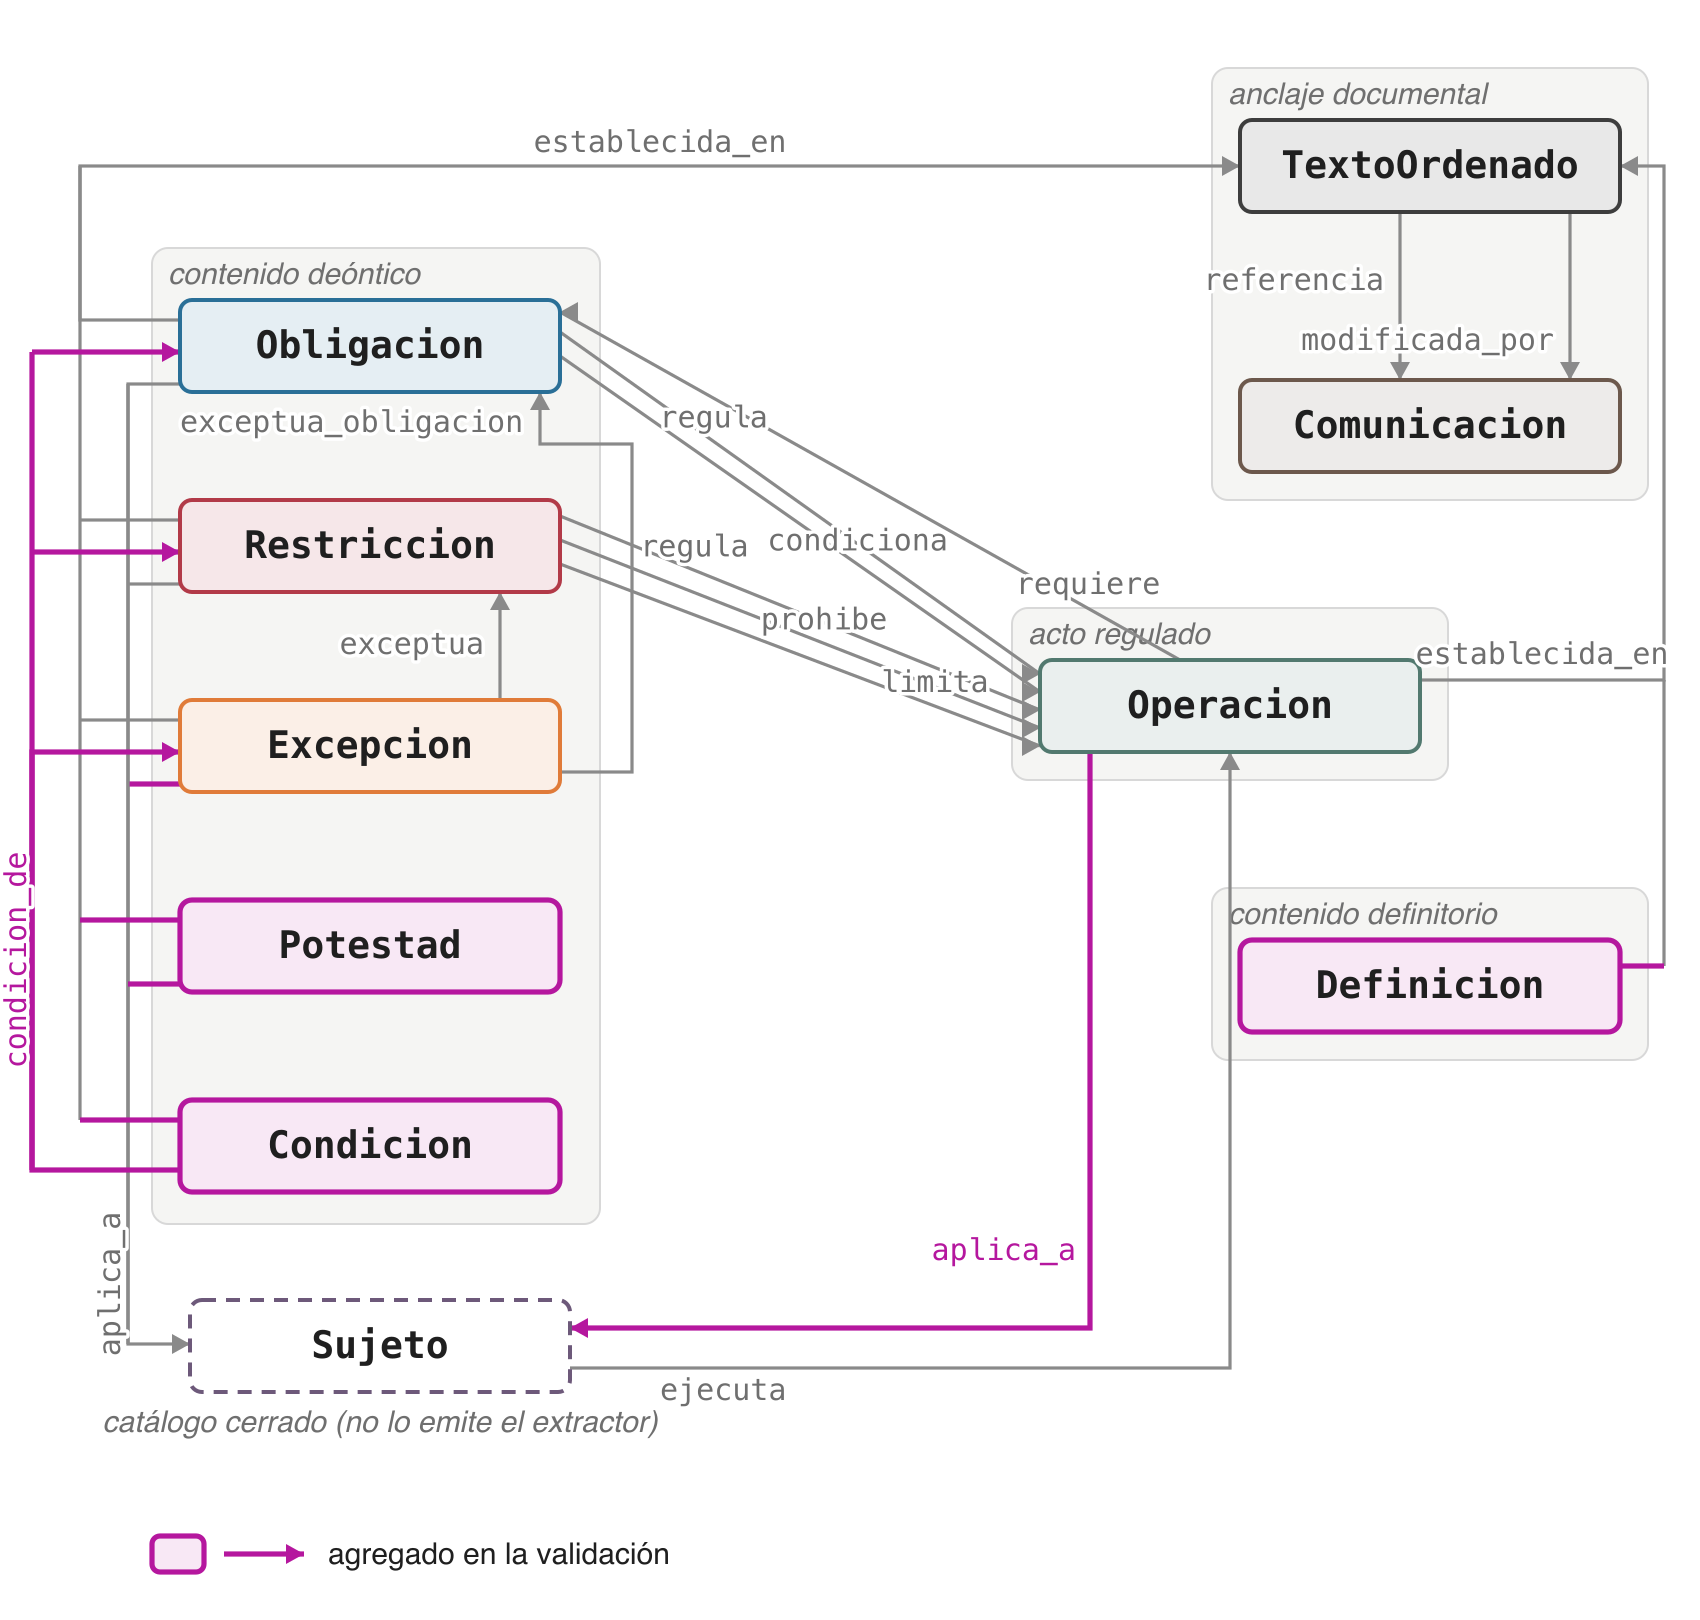
\includegraphics[width=0.85\linewidth]{figuras/figura_esquema_congelado.png}
  \caption[El esquema congelado]{El esquema congelado, el que se aplica al
    corpus completo. Mismo trazado y mismas convenciones que la
    Figura~\ref{fig:esquema_partida}, para leerlas una contra otra. En trazo
    grueso y color aparte va lo que la enmienda agregó: los tres tipos
    nuevos, las tres flechas de \texttt{condicion\_de} y las seis
    ampliaciones de dominio, tres de \texttt{establecida\_en} y tres de
    \texttt{aplica\_a}. De las 26 flechas que expanden las trece relaciones
    de la matriz, 9 son nuevas respecto del esquema de partida. El sujeto
    sigue proviniendo del catálogo cerrado y no lo emite el extractor.}
  \label{fig:esquema_congelado}
\end{figure}

Que los límites se escriban en lugar de resolverse responde a una distinción fijada antes de aplicarla, la misma que en la sección anterior separó a la condición del valor de enumeración que se retiró. Una omisión queda a la vista y se cuenta en la cifra de contenido no representado. Una afirmación falsa que respeta el vocabulario es invisible, justamente porque valida. Por eso ningún cambio que produjera la segunda quedó en el esquema, y sí quedaron, con el residuo declarado, los que solo dejan la primera. El esquema congelado queda con ocho límites escritos. Cuatro son límites del vocabulario, tres de ellos conclusiones de diseño de este trabajo y uno diferido a una versión posterior; tres son conteos que el escalado vuelve a medir; y uno es una propiedad del extractor y no del vocabulario.

El primer límite es que el esquema no representa hechos con valor, los que atan un sujeto, una relación y un valor, como los umbrales y plazos de los que depende que una norma se aplique. Ese contenido queda escrito dentro de la descripción del nodo y no en un campo propio, y el cambio que pediría, atributos en las relaciones, tampoco cubriría el caso en que el hecho tiene más de un valor. La medición lo vio en cuatro fichas de cuatro documentos, las cuatro de la muestra dirigida, y por eso no lo promovió. El capítulo~\ref{sec:conclusiones} lo retoma como límite del modelo de datos.

El segundo es el alcance de la condición, que cubre solo el supuesto enunciado dentro de la misma unidad. Su predicción principal, una condición que remite a otra unidad, falló en las dos vueltas de verificación, y por eso entró con ese alcance y no con el que la lectura había pedido. El remedio queda para una versión posterior del esquema y está declarado en la etapa del verificador, no en la del extractor.

El tercero es la regla que deja fuera el contenido meta-normativo, y falla en las dos direcciones. La misma cláusula interpretativa produjo una prohibición inexistente en las dos corridas medidas, y una unidad de disposiciones transitorias quedó omitida con costo. La regla se conserva porque, cuando actúa, deja una omisión que se cuenta, y su falla en la otra dirección queda declarada como límite en lugar de corregirse con vocabulario nuevo, que es la distinción con la que abre esta sección.

El cuarto es que las obligaciones del corpus no se dejan tipar con una lista cerrada. De los 236 grupos de obligaciones sin tipo asignado, 233 quedan bajo el corte de frecuencia fijado antes de mirarlos, de modo que la enumeración de seis valores describe a las frecuentes y deja a la cola larga con el valor genérico. Ampliar la lista no la agotaría, y el capítulo~\ref{sec:conclusiones} lo trata como propiedad del corpus antes que del esquema.

Tres conteos más no son límites del vocabulario sino tasas que el escalado vuelve a medir contra las de esta validación como línea de base. Son la conversión de una deformación en omisión, con 2 unidades vacías con contenido normativo sobre 43 en la primera vuelta y 2 sobre 27 en la segunda; la migración de un deber a la condición, con 1 caso incorrecto y 1 correcto sobre las 12 unidades de la regresión; y el mismo contenido escrito en dos cajas, persistente sobre una unidad pese a la cláusula que lo prohíbe. Ninguno lleva umbral, porque lo que puede reabrir el esquema no es que un conteo suba sino que el escalado revele una clase de falla que esta validación no vio, y el capítulo~\ref{cap:construccion} los reporta con la primera tanda. 

El octavo límite no es del vocabulario sino del extractor. La calidad de una emisión no se conserva entre corridas aunque el tipo sí, y la validación lo documentó por casos y sin denominador, con un término definido truncado a la mitad, dos contenidos heterogéneos fundidos en uno y una unidad que perdió las doce relaciones que colgaban de un mismo acto regulado. Ningún cambio de esquema lo corrige. La sección~\ref{sec:ensamblado} describe el mecanismo y lo mide sobre las re-extracciones del conjunto de desarrollo, y el capítulo~\ref{sec:conclusiones} lo retoma como límite del proceso de extracción.

Queda un riesgo que ninguno de esos límites cubre. El esquema congelado está informado por 15 de los 157 Textos Ordenados, los 5 del conjunto de desarrollo y los 10 del conjunto de validación, y no se lo probó sobre material que no haya intervenido en él. El riesgo quedó declarado por escrito al congelar el esquema, junto con las razones por las que se lo consideró aceptable.

Tres de esas razones se sostienen. Los dos patrones que el criterio promovió aparecen en cinco y en diez documentos, así que ningún tipo nuevo persigue una aparición aislada. El criterio sellado descartó lo débil, y los patrones y las familias que aparecieron una sola vez quedaron como residuo en lugar de convertirse en vocabulario. Y los tres tipos que entraron son categorías del derecho antes que rasgos de estos documentos, lo que hace menos probable que sean idiosincrasias de los quince leídos.

Las otras dos razones prometían más de lo que prueban, y la corrección quedó registrada. La primera decía que la regresión de la segunda vuelta se había corrido sobre material fresco. Lo es a nivel de unidad, porque ninguna ficha había mirado esas doce, pero no a nivel de documento, porque salen de los mismos diez que informaron los cambios. Lo que esa regresión muestra es que las cajas nuevas no atraen contenido indebido en documentos que el esquema ya conocía; no dice qué harían en documentos que nunca vio. La segunda decía que la primera tanda del escalado sería el test de generalización. Lo es solo si sus documentos se eligen entre los 58 que quedan al sacar los diez del conjunto de validación de los 68 que la segmentación reconoce sin reglas adicionales; con cualquier otro recorte vuelve a entrar material que ya intervino en el esquema.

Para el catálogo de sujetos no hay recorte que sirva. Los 68 documentos de ese grupo se leyeron para el catálogo, 66 con su pasaje de alcance y su entrada escrita a partir de esa lectura y 2 declarados sin pasaje, de modo que ninguno es material no visto para el catálogo. La sección~\ref{sec:extension_catalogo} vuelve sobre ese punto con el catálogo escalado.

\chapter{Construcción del grafo}
\label{cap:construccion}

\section{La extensión del catálogo de sujetos}
\label{sec:extension_catalogo}

El catálogo con el que se validó el esquema tiene 70 entradas y cubre los cinco documentos del conjunto de desarrollo. Antes de extraer el resto del corpus hubo que extenderlo, y la extensión no salió de las propuestas que el modelo había dejado en cuarentena sino de leer los documentos. Se leyó el pasaje de alcance de cada uno de los 68 cuya estructura la segmentación reconoce sin reglas adicionales. En 36 ese pasaje nombra una clase que el catálogo ya tenía, y el documento se mapeó a ella. En 30 nombra un colectivo que ninguna clase cubre sola, y el documento recibió un rol de alcance propio. Los dos restantes quedaron declarados sin entrada, con el campo de propuesta abierto. Se sumaron además siete sujetos nuevos, cada uno con su evidencia citada en el texto, y se retiraron cinco entradas sin uso medido, de modo que el catálogo escalado queda en 102 entradas. Los doce documentos no segmentables no entraron en ese reparto y no tienen rol propio.

La extensión no cubre todo lo que los documentos nuevos nombran. Al declarar a quién se dirigen, esos 30 documentos mencionan 69 grupos distintos, y solo 34 tienen en el catálogo una clase que les corresponda, el 49,3\,\%. De los 35 restantes, 26 nombran algo que el catálogo no contempla y los otros 9 lo contemplan a un nivel de generalidad distinto. Doce de los 30 roles quedan por eso sin miembros declarados, sea porque el grupo no tiene entrada o porque aplanarlo a una clase más amplia se rechazó, y cada caso está registrado con su causa.

Esta extensión tiene un costo declarado. Los diez documentos del conjunto de validación están entre esos 68, así que a los diez se les leyó el pasaje de alcance y de esa lectura salió su entrada de catálogo; cinco recibieron además un rol propio, y aportan 13 de los 69 grupos. Material reservado para medir el esquema intervino por esa vía en la construcción del catálogo con el que se extrae el corpus completo, y por eso la sección~\ref{sec:limites} declara que el catálogo no puede evaluarse sobre ninguno de esos documentos.

\section{Los documentos no segmentables}
\label{sec:cobertura_no_segmentables}

Que un documento no se deje segmentar no significa que no contenga norma. De los doce declarados no segmentables en la sección~\ref{sec:segmentacion}, nueve se cortaron por página en lugar de por punto, con la página como unidad y como procedencia. Eso dio 77 unidades de prosa y 114 de planilla. Las de prosa ingresan al grafo al ensamblar el corpus escalado y reemplazan a las diez unidades sin estructura que esos nueve documentos aportaban al conteo de la sección~\ref{sec:segmentacion}, con lo que el recurso pasa de 9.324 unidades a 9.391. Las de planilla quedan medidas y fuera, para una etapa posterior. Los tres documentos restantes quedan afuera por razones distintas. Dos no prescriben, y se adjudicaron como texto de referencia sin obligaciones ni restricciones que extraer. El tercero sí prescribe, pero tiene numeración propia que la segmentación reconoce solo en parte, y tratarlo por página le daría una procedencia más gruesa que la que el documento admite.

\section{La extracción a escala}
\label{sec:extraccion_escala}
% Pendiente de la primera tanda del escalado sobre los 68 documentos.
% Alimenta: reporte de tanda 1, con los ítems de vigilancia de la
% limites medidos contra sus tasas de línea de base.

\section{El ensamblado y el verificador}
\label{sec:ensamblado}
% Pendiente. Alimenta: rechazos por firma en E2, nodos de sujeto, cola
% humana; comportamiento de E3 en desarrollo (330 unidades re-extraídas,
% 61 con menos entidades o relaciones que la primera pasada, 80 a cola).

% Verificar la firma es una comprobación determinística, sin modelo, y cada relación rechazada queda registrada con la firma que intentó y con la salida íntegra del modelo al lado, de modo que el rechazo es recontable en cualquier momento

\section{El grafo resultante}
\label{sec:grafo_resultante}
% Pendiente. Alimenta: kg.json de la tanda, nodos y aristas por tipo.

% Pendiente. Acá va la regla de versiones que salió de la Introducción
% (comentario rojo, 17/09): el grafo que se evalúa se reporta tal como fue
% construido; las correcciones que la evaluación motive se incorporan en una
% versión posterior, que es la que se publica; una corrección nunca se aplica
% sobre el grafo ya evaluado para mejorar su número. Se enuncia una vez acá y
% la Conclusión la retoma como limitación de método, no en la Introducción.

%este era el comentario y el parrafo que saque:
%El proceso se desarrolló sobre cinco Textos Ordenados, el conjunto de desarrollo; el esquema se puso a prueba sobre otros diez antes de escalar, y el recurso final se construye sobre el corpus completo. El grafo que se evalúa se reporta tal como fue construido; las correcciones que la evaluación motive se incorporan en una versión posterior, que es la que se publica \textcolor{red}{Esto no se si lo pondria aca te baja el precio}
% [TODO: escalado] cuando exista el grafo escalado, "el recurso final se
% construye sobre el corpus completo" pasa a decir su escala.
% La elección de esquema cerrado se justifica en el capítulo~\ref{cap:esquema}
% El alcance exacto del escalado depende del laudo D5 (pendiente; base no disputada: 68 TOs digeribles primero).


\section{Las guardas selladas}
\label{sec:guardas}

El escalado lleva predicciones selladas antes de correr, y la primera que se resolvió fue sobre las 77 unidades de prosa de los documentos no segmentables. Esas unidades se extrajeron con el esquema congelado y el catálogo de 102 entradas, y sin rol de alcance propio, porque sus documentos no lo tienen. Antes de extraerlas quedó fijado un piso: la fracción de unidades con al menos una arista hacia su destinatario no podía caer por debajo del 42,9\,\%, que son las 33 de las 77 en cuyo texto aparece literalmente un sujeto del catálogo. La consecuencia de no alcanzarlo también estaba declarada, y era que la prosa ingresara igual, con la tasa de cada documento publicada contra su propia tasa literal y sin excluir ningún documento. La medición dio 13 de 77, el 16,9\,\%, y la predicción falló.

La adjudicación posterior mostró que el piso estaba mal especificado. Se había fijado contando esas 33 menciones léxicas como si todas fueran destinatarios de la norma, y la lectura caso por caso encontró que la mayoría no lo era, sino definiciones, remisiones y menciones de paso. Sobre los destinatarios que el texto efectivamente da, las 77 unidades aportan 18. De las trece unidades que habían emitido arista, una quedó sin ninguna, porque las dos que llevaba ataban la norma a un sujeto que el pasaje no obliga, y una afirmación de esa clase es falsa en un campo estructurado, de modo que se retiró en lugar de aceptarse con residuo. Quedan 12 unidades con destinatario emitido sobre los 18 que el texto da, el 66,7\,\%, y seis sin el destinatario que su propio texto nombraba.

La revisión de esta guarda encontró además dos defectos de especificación que la adjudicación no había visto. El piso se calculó contando menciones contra el catálogo de 70 entradas, mientras la extracción corrió con el de 102. Y el techo del intervalo, 53,1\,\%, se tomó del conjunto de desarrollo, cuyos cinco documentos llevan rol de alcance, mientras estos nueve corrieron sin rol, y el diseño de la validación ya había dejado escrito que una tasa con rol y una sin rol no son comparables. Ninguno de los dos cambia el 12 de 18, que se leyó contra el texto y no contra el intervalo, pero los dos muestran que la predicción sellada tenía más de un error.

El ancla mal especificada se descubrió porque estaba sellada y la predicción falló contra una guarda. Con un umbral elegido después de ver los datos, la medición habría pasado sin que nadie advirtiera que contaba definiciones como destinatarios, que comparaba contra un catálogo distinto del que corrió, ni que tomaba su techo de una población que no se le parece.

\chapter{Evaluación de fidelidad}
\label{cap:fidelidad}

\section{El agente y el sistema de consulta}
\label{sec:sistema}
% PROMESAS DEL MARCO TEÓRICO QUE ESTA SECCIÓN CIERRA
% 2.3.2 -> tres herramientas, tope, abstención
% 2.3.3 -> qué índice de texto usó cada medición
% 2.4.2 -> juez, criterios, validaciones con cifras
%
% 5.1.1 Las tres herramientas
%   buscar_nodos(consulta, limite), ver_nodo(id), ver_vecinos(id, direccion)
%   harness.py:240-286; modelo claude-haiku-4-5, temperatura 0
% 5.1.2 El tope y la abstención
%   MAX_TOOL_CALLS = 15, se controla al cierre de cada turno, por eso
%   un turno puede excederlo: 80 de 456 trazas de EV2 lo superaron, máximo 18
%   abstención = respondible:false en la salida (puede llevar citas igual)
% 5.1.3 El índice de texto detrás de buscar_nodos
%   todas las mediciones de desarrollo de EV2 (base, re-corridas de §7, r1)
%   usaron GraphIndex en memoria, intersección de tokens, sin pesos ni stemming
%   Neo4j 5.26.9 con índice fulltext (analizador spanish, campos label,
%   descripcion, description, id_texto; Lucene BM25 por defecto) se usó en la
%   ablación A1.4 (400 trazas), el banco MCP, la aplicación y el escalado
%   (laudo A1.6, docs/decision_backend_grafo.md); decir cuál usa cada tabla
% 5.1.4 Qué se guarda de cada corrida
%   steps, seen_provenances, citations_unseen_raw/normalized, final_json,
%   cost, latency; el runner de EV2 persiste además steps_full y raw_turns
% 5.1.5 El juez y sus validaciones
%   claude-sonnet-4-6, temperatura 0, prompt sha fd446f8e, unidad
%   (respuesta, criterio), tres corridas y voto modal, ciego
%   mapping.py:40-54: dudoso o sin consenso -> requiere adjudicación;
%   todos cumplidos -> correcta; todos no cumplidos -> incorrecta; resto parcial
%   validación U6: 25 respuestas, 92 criterios, 14 acuerdos, 6 desacuerdos,
%   5 a adjudicación; v1.1 rechazada por el candado (3 de 91 cambios)
%   muestra simétrica ciega: 12 fichas, 53 criterios, 11/12 y 52/53,
%   único desacuerdo juez parcial / humana correcta, adjudicado a ciegas
%   hoja de trabajo 48/200 con 30 requiere adjudicación, resueltos 20/17

\chapter{Atribución causal de fallas}
\label{cap:atribucion}

\chapter{Comparación contra recuperación por fragmentos}
\label{cap:comparacion}

\chapter{Evaluación intrínseca del grafo}
\label{cap:intrinseca}

\chapter{Explicabilidad de restricciones operativas}
\label{cap:explicabilidad} %--> cuando este hecho lo agrego a contribuciones


\chapter{Conclusiones y trabajo futuro}
\label{sec:conclusiones}
% PPT (diapo Conclusión): discutir resultados y contrastarlos con
% resultados previos; importancia Y limitaciones; si se lograron los
% objetivos de la introducción; qué estudios futuros se abren.
% Guía CEU: la conclusión reafirma la introducción — cerrar contra los
% objetivos específicos declarados arriba.
% Temas reales de esta tesis para trabajo futuro [TODO: validar lista]:
% escalado al corpus BCRA completo, r2 con correcciones trazadas a
% hallazgos, E4-LLM para los 196 conflictos persistidos, rangos→contenedor,
% actualización incremental ante normativa nueva, y versionado temporal
% (vigencias, norma que modifica o deroga a otra; modificada_por hoy con
% 0 ocurrencias; sin preguntas as-of-date en el conjunto de evaluación).

% --- BIBLIOGRAFIA ---
\chapter{Bibliografía}
\printbibliography[heading=none]

% --- APÉNDICES ---
% PPT: material complementario, tablas, código. Candidatos naturales:
% protocolo EV2, pre-registros, prompts sellados, tabla de hallazgos H1-H26.
\appendix


\end{document}